\chapter{HASIL DAN PEMBAHASAN}

\vspace{1cm}
\section{Area Studi}
\hspace{1,2cm}
Terdapat dua area studi yang dilakukan pada penelitian ini, yaitu Kebun Pendidikan dan Penelitian Kelapa Sawit milik Institut Pertanian Bogor-Cargil yang berlokasi di Jonggol, Jawa Barat dan Universitas Gunadarma di Penajam Paser Utara, Kalimantan Timur yang memiliki lahan yang ditanami pohon kelapa sawit.

Area studi ini secara umum mencakup untuk pengambilan data citra pohon kelapa sawit sebagai dataset primer. Tabel \ref{tbl:Data-Lokasi-dan-Luasan-Area-Studi} menampilkan lokasi koordinat dan luasan lahan yang diambil sebagai citra pohon kelapa sawit.

%%%%%%%%%%%%%%%%%%%%%%%TABEL SEDERHANA%%%%%%%%%%%%%%%%%%%%%%%%%
\begin{singlespace}
	\begin{table}[H]
		\centering
		\caption{Data Lokasi dan Luasan Area Studi}
		\label{tbl:Data-Lokasi-dan-Luasan-Area-Studi}
		\begin{tabular}{|p{4cm}|p{4cm}|p{4cm}|}
			\hline
			\rowcolor[HTML]{D9D9D9}
			Area Studi                                                                         & Lokasi Koordinat (Latitude, Longitude) & Luasan Lahan (ha) \\ \hline

			Kebun Pendidikan dan Penelitian Kelapa Sawit milik Institut Pertanian Bogor-Cargil & -6.4277942, 106.8418378                                                          & 63,48                                                          \\ \hline
			
			Universitas Gunadarma di Penajam Paser Utara, Kalimantan Timur                     & -1.318495, 116.6678405                                                           & $\approx$ 18                                                           \\ \hline
			\end{tabular}
	\end{table}
\end{singlespace}
%%%%%%%%%%%%%%%%%%%%%%%TABEL SEDERHANA%%%%%%%%%%%%%%%%%%%%%%%%%

Pengambilan citra pada area studi diambil dengan menggunakan DJI Mavic 2 Pro dari ketinggian 100 m di atas permukaan tanah dengan pakar atau pilot drone yang sudah tersertifikasi. Pada tahap pengujian pada sistem untuk mendeteksi dan menghitung, serta titik koordinat latitude-longitude dari setiap pohon kelapa sawit menggunakan area Kebun Pendidikan dan Penelitian Kelapa Sawit milik Institut Pertanian Bogor-Cargil Blok 1, 2, 3, dan 4. Pada proses pengambilan citra untuk dataset primer pada area studi lahan pada Kebun Pendidikan dan Penelitian Kelapa Sawit milik Institut Pertanian Bogor-Cargil berhasil ditangkap area blok 3 dan 4 dari total 4 blok. Peta sebaran area inisialisasi lahan pada kebun ini seperti pada Gambar \ref{img:Peta-Sebaran-Area-Inisialisasi-Lahan-Kebun} yang memiliki 5670 pohon tanam kelapa sawit berdasarkan hasil wawancara di lapangan pada area studi Kebun Pendidikan dan Penelitian Kelapa Sawit milik Institut Pertanian Bogor-Cargil.

%%%%%%%%%%%%%%%%%%%%%%%%%% GAMBAR %%%%%%%%%%%%%%%%%%%%%%%%%%%%%%
\begin{figure}[H]
	\vspace{-0.1cm}
	%\rule{\columnwidth}{0.1pt}
	\begin{center}
		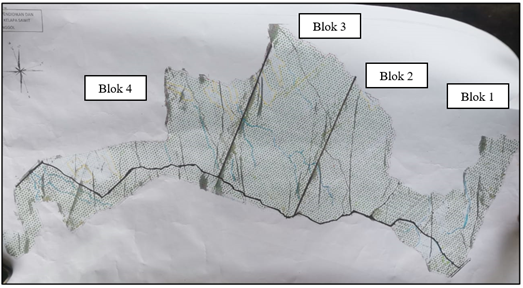
\includegraphics[width=1\columnwidth]{bab4/Gambar/Picture1.png}
	\end{center}
	\vspace{-0.2cm}
	%\rule{\columnwidth}{0.1pt}
	\captionsetup{justification=centering}
	\caption{Peta Sebaran Area Inisialisasi Lahan Kebun Pendidikan dan Penelitian Kelapa Sawit milik Institut Pertanian Bogor-Cargil}\label{img:Peta-Sebaran-Area-Inisialisasi-Lahan-Kebun}
\end{figure}
%%%%%%%%%%%%%%%%%%%%%%%%%% GAMBAR %%%%%%%%%%%%%%%%%%%%%%%%%%%%%%

Area lahan yang berhasil ditangkap pada kebun ini berada pada area studi blok 3 dan blok 4. Area studi yang digunakan untuk dataset primer yang digunakan blok 3 pada Gambar 3.6 dan blok 4 pada Gambar 3.7. dengan total luas sebesar 37,51 hektar, dan pengujian digunakan blok 1 (Gambar 4.2), 2 (Gambar 4.3), 3, dan 4 seperti pada Tabel \ref{tbl:Area-Studi-Yang-Berhasil-Ditangkap-Menjadi-CItra-Area-Pohon-Kelapa-Sawit-Dengan-Drone} dengan total luas area 63,48 hektar pada Kebun Pendidikan dan Penelitian Kelapa Sawit Institut Pertanian Bogor-Cargil dengan perhitungan luas area menggunakan bantuan layanan DroneDeploy.

%%%%%%%%%%%%%%%%%%%%%%%TABEL SEDERHANA%%%%%%%%%%%%%%%%%%%%%%%%%
\begin{singlespace}
	\begin{table}[H]
		\centering
		\caption{Area Studi yang Berhasil Ditangkap menjadi Citra Area Pohon Kelapa Sawit dengan Drone}
		\label{tbl:Area-Studi-Yang-Berhasil-Ditangkap-Menjadi-CItra-Area-Pohon-Kelapa-Sawit-Dengan-Drone}
		\begin{tabular}{|ll|l|}
			\hline
			\rowcolor[HTML]{D9D9D9} 
			\multicolumn{1}{|l|}{\cellcolor[HTML]{D9D9D9}No.} & Area   & Luas Area (ha) \\ \hline
			\multicolumn{1}{|l|}{1}                           & Blok 1 & 14,66          \\ \hline
			\multicolumn{1}{|l|}{2}                           & Blok 2 & 11,31          \\ \hline
			\multicolumn{1}{|l|}{3}                           & Blok 3 & 18,20          \\ \hline
			\multicolumn{1}{|l|}{4}                           & Blok 4 & 19,31          \\ \hline
			\multicolumn{2}{|l|}{Total}                                & 63,48          \\ \hline
		\end{tabular}
	\end{table}
\end{singlespace}
%%%%%%%%%%%%%%%%%%%%%%%TABEL SEDERHANA%%%%%%%%%%%%%%%%%%%%%%%%%

%%%%%%%%%%%%%%%%%%%%%%%%%% GAMBAR %%%%%%%%%%%%%%%%%%%%%%%%%%%%%%
\begin{figure}[H]
	\vspace{-0.1cm}
	%\rule{\columnwidth}{0.1pt}
	\begin{center}
		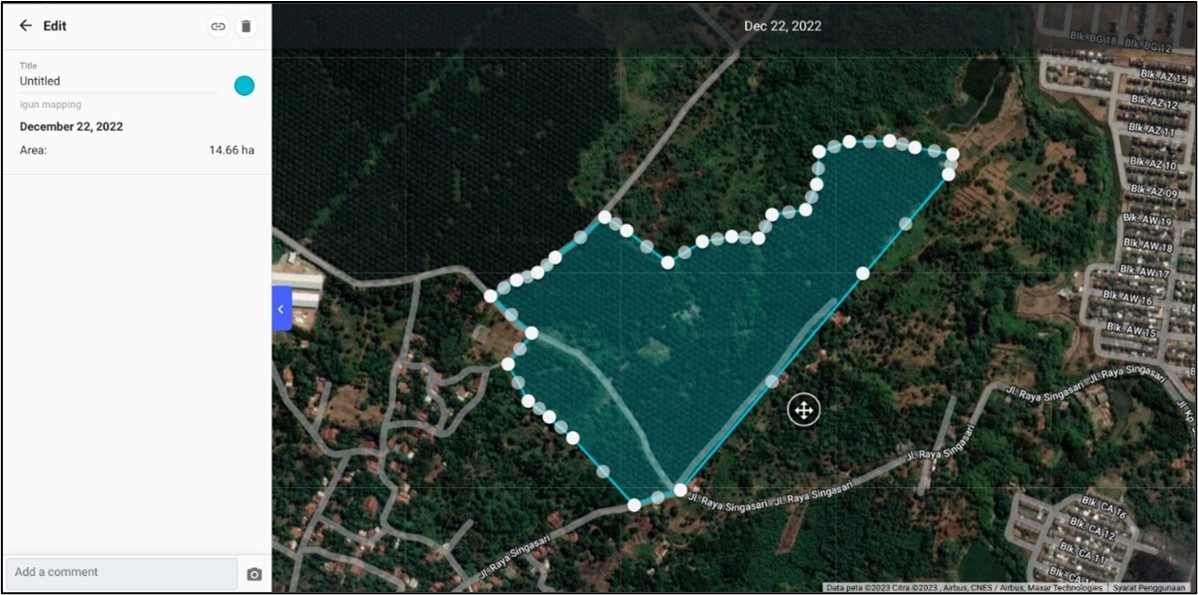
\includegraphics[width=0.7\columnwidth]{bab4/Gambar/Picture2.jpg}
	\end{center}
	\vspace{-0.2cm}
	%\rule{\columnwidth}{0.1pt}
	\captionsetup{justification=centering}
	\caption{Luas Area Blok 1 Kebun Pendidikan dan Penelitian Kelapa Sawit Institut Pertanian Bogor-Cargil}\label{img:Luas-Area-Blok-1-Kebun-Pendidikan}
\end{figure}
%%%%%%%%%%%%%%%%%%%%%%%%%% GAMBAR %%%%%%%%%%%%%%%%%%%%%%%%%%%%%%

%%%%%%%%%%%%%%%%%%%%%%%%%% GAMBAR %%%%%%%%%%%%%%%%%%%%%%%%%%%%%%
\begin{figure}[H]
	\vspace{-0.1cm}
	%\rule{\columnwidth}{0.1pt}
	\begin{center}
		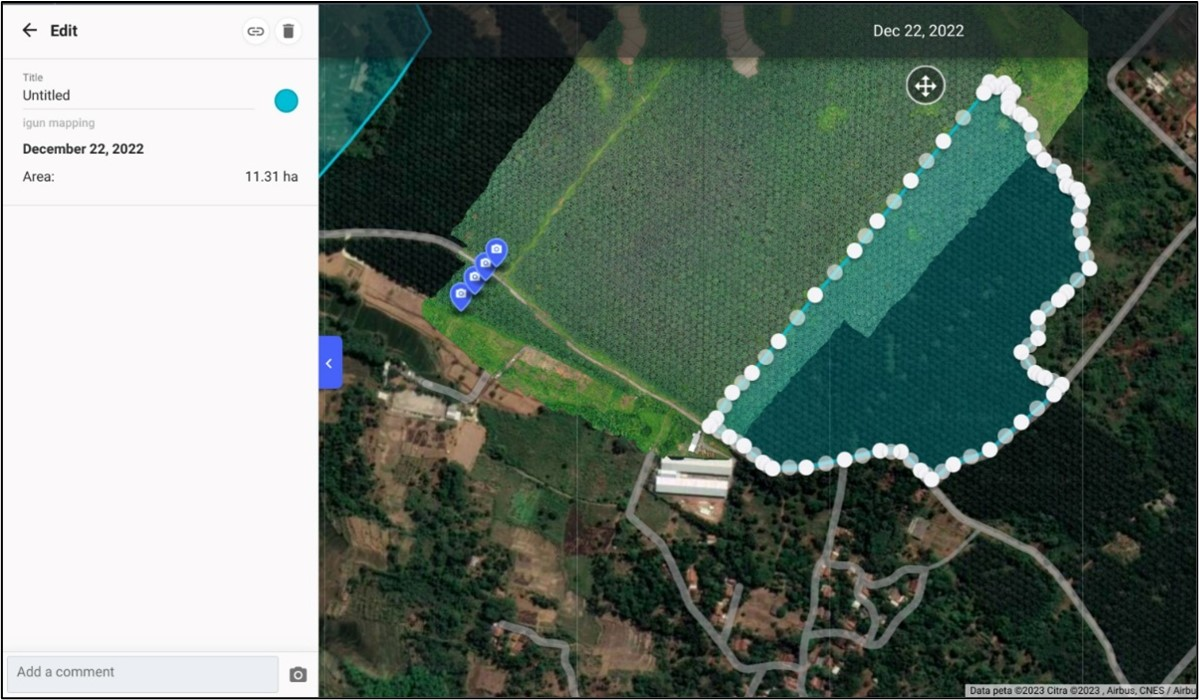
\includegraphics[width=0.7\columnwidth]{bab4/Gambar/Picture3.jpg}
	\end{center}
	\vspace{-0.2cm}
	%\rule{\columnwidth}{0.1pt}
	\captionsetup{justification=centering}
	\caption{Luas Area Blok 2 Kebun Pendidikan dan Penelitian Kelapa Sawit Institut Pertanian Bogor-Cargil}\label{img:Luas-Area-Blok-2-Kebun-Pendidikan}
\end{figure}
%%%%%%%%%%%%%%%%%%%%%%%%%% GAMBAR %%%%%%%%%%%%%%%%%%%%%%%%%%%%%%

\section{Persiapan Data}
\hspace{1,2cm}
Persiapan data, yang dikenal dengan \textit{data preprocessing} adalah tahap yang penting untuk menyiapkan data untuk dapat digunakan dalam modeling dengan \textit{deep learning}. Persiapan data meliputi persiapan dataset primer dan sekunder untuk dapat digunakan.

\subsection{Deskripsi Dataset dan Pemilihan}
\hspace{1,2cm}
Akuisisi citra area pohon kelapa sawit menjadi penting karena berhubungan hasil memindai, menangkap (\textit{capture}), atau menjadi suatu foto citra yang dapat digunakan untuk dataset. Citra area pohon kelapa sawit pada penelitian ini dibagi menjadi dua, yaitu citra untuk dataset primer dan sekunder.

\subsubsection{Dataset Primer}
\hspace{1,2cm}
Dataset primer digunakan untuk membangun atau memberikan anotasi atau label oil palm pada citra gambar. Hasil gambar citra pohon kelapa sawit dari dua area studi memiliki format citra yang sama, yaitu *.jpg. Data citra dari Kebun Pendidikan dan Penelitian Kelapa Sawit milik Institut Pertanian Bogor-Cargil yang diambil dari blok 3 dan 4 terdiri dari 69 citra atau gambar, sedangkan jumlah citra yang dihasilkan dari area kelapa sawit berjumlah 205 citra dengan dimensi ukuran citra sebesar 5472 x 3078 px, seperti pada Tabel \ref{tbl:Jumlah-Citra-Dari-Dua-Area-Studi}

Total citra dataset primer dari dua area studi seperti pada Tabel \ref{tbl:Jumlah-Citra-Dari-Dua-Area-Studi} berikut.

%%%%%%%%%%%%%%%%%%%%%%%TABEL SEDERHANA%%%%%%%%%%%%%%%%%%%%%%%%%
\begin{singlespace}
	\begin{table}[H]
		\centering
		\caption{Jumlah Citra dari Dua Area Studi}
		\label{tbl:Jumlah-Citra-Dari-Dua-Area-Studi}
		\begin{tabular}{|p{4cm}|p{4cm}|p{4cm}|}
			\hline
			\rowcolor[HTML]{D9D9D9} 
			Area Studi                                                                         & Jumlah Citra & Luas Area (ha) \\ \hline
			Kebun Pendidikan dan Penelitian Kelapa Sawit milik Institut Pertanian Bogor-Cargil & 69           & 14,66          \\ \hline
			Universitas Gunadarma di Penajam Paser Utara, Kalimantan Timur                     & 205          & 11,31          \\ \hline
		\end{tabular}
	\end{table}
\end{singlespace}
%%%%%%%%%%%%%%%%%%%%%%%TABEL SEDERHANA%%%%%%%%%%%%%%%%%%%%%%%%%

Hasil citra dari area studi Universitas Gunadarma dengan jumlah 205 citra atau gambar ini digunakan untuk dataset primer dengan memberikan anotasi atau pemberian label secara otomatis yang dilakukan dalam penelitian ini.  Adapun citra sampel area studi dari Universitas Gunadarma tampak pada Gambar \ref{img:Hasil-Citra-Sampel-Universitas-Gunadarma-1} dan citra sampel Kebun Pendidikan dan Penelitian Kelapa Sawit milik Institut Pertanian Bogor-Cargil tampak pada Gambar \ref{img:Hasil-Citra-Sampel-Universitas-Gunadarma-2}

%%%%%%%%%%%%%%%%%%%%%%%%%% GAMBAR %%%%%%%%%%%%%%%%%%%%%%%%%%%%%%
\begin{figure}[H]
	\vspace{-0.1cm}
	%\rule{\columnwidth}{0.1pt}
	\begin{center}
		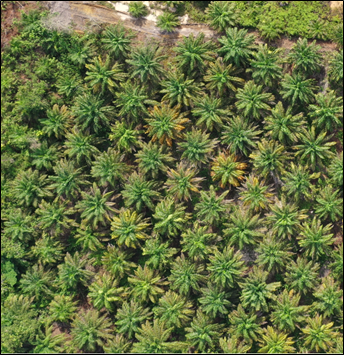
\includegraphics[width=0.6\columnwidth]{bab4/Gambar/Picture4.1.png}
		\hspace{1cm}
		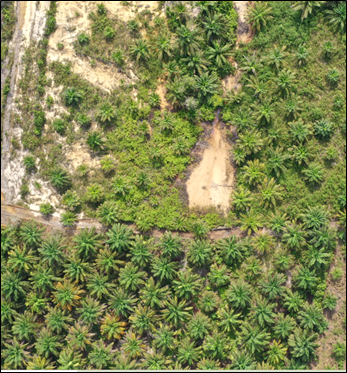
\includegraphics[width=0.6\columnwidth]{bab4/Gambar/Picture4.2.png}
	\end{center}
	\vspace{-0.2cm}
	%\rule{\columnwidth}{0.1pt}
	\captionsetup{justification=centering}
	\caption{Hasil Citra Sampel Universitas Gunadarma di Penajam Paser Utara, Kalimantan Timur}\label{img:Hasil-Citra-Sampel-Universitas-Gunadarma-1}
\end{figure}
%%%%%%%%%%%%%%%%%%%%%%%%%% GAMBAR %%%%%%%%%%%%%%%%%%%%%%%%%%%%%%

%%%%%%%%%%%%%%%%%%%%%%%%%% GAMBAR %%%%%%%%%%%%%%%%%%%%%%%%%%%%%%
\begin{figure}[H]
	\vspace{-0.1cm}
	%\rule{\columnwidth}{0.1pt}
	\begin{center}
		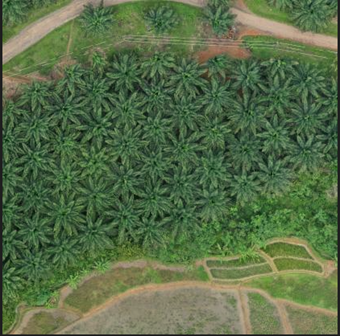
\includegraphics[width=0.6\columnwidth]{bab4/Gambar/Picture5.1.png}
		\hspace{1cm}
		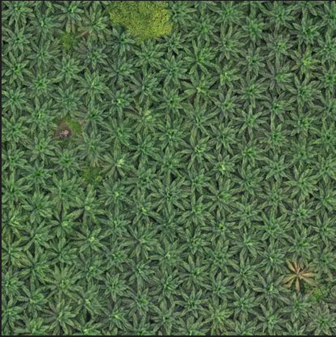
\includegraphics[width=0.6\columnwidth]{bab4/Gambar/Picture5.2.png}
	\end{center}
	\vspace{-0.2cm}
	%\rule{\columnwidth}{0.1pt}
	\captionsetup{justification=centering}
	\caption{Hasil Citra Sampel Universitas Gunadarma di Penajam Paser Utara, Kalimantan Timur}\label{img:Hasil-Citra-Sampel-Universitas-Gunadarma-2}
\end{figure}
%%%%%%%%%%%%%%%%%%%%%%%%%% GAMBAR %%%%%%%%%%%%%%%%%%%%%%%%%%%%%%

\subsubsection{Dataset Sekunder}
\hspace{1,2cm}
Data sekunder yang digunakan sudah memiliki label atau anotasi sebagai pohon kelapa sawit "oil palm". Data berjumlah 1795 citra yang sudah memiliki kotak batas atau \textit{bounding box} dengan kelas \textit{oil palm}. Data sekunder digunakan untuk menambah data pada sata proses pelatihan, validasi dan pengujian. Data tersebut semakin bervariasi, maka keterwakilan data pada citra yang berupa objek pohon kelapa sawit semakin baik. Dataset sekunder dapat diakses secara daring dan dapat digunakan secara \textit{free} atau \textit{open source} melalui sistem berbasis web bernama roboflow.

GAMBAR

Data sample pada dataset sekunder yang sudah memiliki \textit{bounding box} yang diberi label oil palm, seperti pada Gambar 4.6.

Dataset sekunder ini dilakukan proses augmentasi dengan menggunakan bantuan layanan roboflow. Proses augmentasi ini dilakukan untuk menambah banyaknya data citra, serta bertujuan agar mesin dapat belajar dan mengenali dari berbagai citra yang berbeda-beda. Penggunaan augmentasi ini diharapkan dapat meningkatkan performa dari model, karena mesin yang digunakan dalam penelitian ini agar dapat berhasil mengenali lebih banyak objek dari bentuk dan pola yang beragam jenis data citra. 

Data sekunder ini berada pada layanan roboflow dan memiliki fasilitas layanan untuk augmentasi. Proses augmentasi dilakukan dengan menambahkan data citra dari data sekunder, seperti pada Gambar 4.7.

%%%%%%%%%%%%%%%%%%%%%%%%%% GAMBAR %%%%%%%%%%%%%%%%%%%%%%%%%%%%%%
\begin{figure}[H]
	\vspace{-0.1cm}
	%\rule{\columnwidth}{0.1pt}
	\begin{center}
		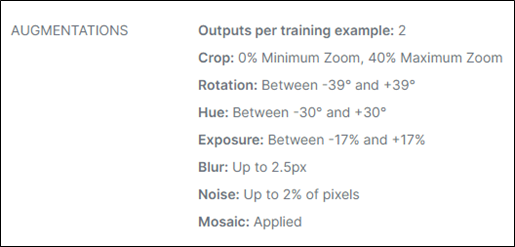
\includegraphics[width=1\columnwidth]{bab4/Gambar/Picture7.png}
	\end{center}
	\vspace{-0.2cm}
	%\rule{\columnwidth}{0.1pt}
	\captionsetup{justification=centering}
	\caption{Proses Augmentasi Data Sekunder }\label{img:Proses-Augmentasi-Data-Sekunder}
\end{figure}
%%%%%%%%%%%%%%%%%%%%%%%%%% GAMBAR %%%%%%%%%%%%%%%%%%%%%%%%%%%%%%

Fitur layanan augmentasi yang digunakan antara lain \textit{crop, rotation, hue, exposure, blur, noise, dan mosaic}. Fitur layanan ini memiliki kegunaan yang mewakili kondisi seperti data studi atau lapangan. Kegunaan fitur layanan yang digunakan seperti pada Tabel \ref{tbl:Kegunaan-Layanan-Augmentasi-Dataset-Sekunder}.
	
%%%%%%%%%%%%%%%%%%%%%%%TABEL SEDERHANA%%%%%%%%%%%%%%%%%%%%%%%%%
\begin{singlespace}
	\begin{table}[H]
		\centering
		\caption{Kegunaan Layanan Augmentasi Dataset Sekunder}
		\label{tbl:Kegunaan-Layanan-Augmentasi-Dataset-Sekunder}
		\begin{tabular}{|p{3cm}|p{8cm}|}
			\hline
			\rowcolor[HTML]{D9D9D9} 
			Augmentasi & Kegunaan                                                                                                                                             \\ \hline
			Crop       & Menambahkan variabilitas pada pemosisian dan ukuran untuk membantu model lebih mengenali terhadap translasi subjek dan posisi kamera.                \\ \hline
			Rotation   & Menambahkan variabilitas pada rotasi untuk membantu model agar dapat mendeteksi objek, bahkan saat kamera atau subjek tidak sejajar secara sempurna. \\ \hline
			Hue        & Mengubah warna secara acak untuk membuat model tidak terlalu sensitif.                                                                       \\ \hline
			Exposure & Menambahkan variabilitas pada kecerahan gambar untuk membantu model lebih dapat mengenali terhadap perubahan pencahayaan dan pengaturan kamera. \\ \hline
			Blur & Menambahkan keburaman Gaussian secara acak untuk membantu model lebih mengenali terhadap fokus kamera, jika data citra berada pada area hutan, kebun, dan alam liar, mungkin tidak berada dalam keadaan focus tangkapan citra tersebut. \\ \hline
			Noise & Menambahkan noise untuk membantu model lebih mengenali terhadap noise yang dapat membantu mempertahankan nilai dan menghindari overfitting dari hasil pengujian. \\ \hline
			Mosaic & Menambahkan mosaik untuk membantu model tampil lebih baik pada objek kecil, mosaik menggabungkan beberapa foto dari rangkaian pelatihan data. \\ \hline
		\end{tabular}
	\end{table}
\end{singlespace}
%%%%%%%%%%%%%%%%%%%%%%%TABEL SEDERHANA%%%%%%%%%%%%%%%%%%%%%%%%%

Tabel 4.5 . menampilkan hasil data citra untuk dataset yang telah dilakukan proses augmentasi sesuai dengan Tabel 4.4. dan tampalian data citra yang berbeda dengan data citra dataset sekunder asli seperti pada Gambar \ref{img:Data-Citra-Asli-Data-Sekunder}.

%%%%%%%%%%%%%%%%%%%%%%%%%% GAMBAR %%%%%%%%%%%%%%%%%%%%%%%%%%%%%%
\begin{figure}[H]
	\vspace{-0.1cm}
	%\rule{\columnwidth}{0.1pt}
	%\begin{center}
	%	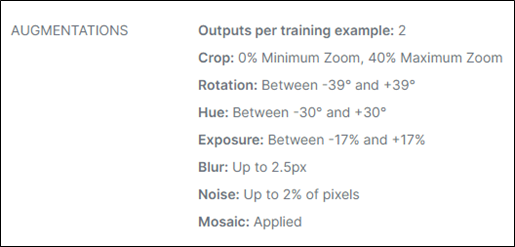
\includegraphics[width=1\columnwidth]{bab4/Gambar/Picture7.png}
	%\end{center}
	\centering
	\subfloat{{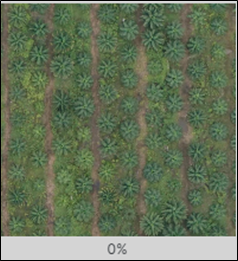
\includegraphics[width=6cm]{bab4/Gambar/Picture8.1.png} }}%
	\qquad
	\subfloat{{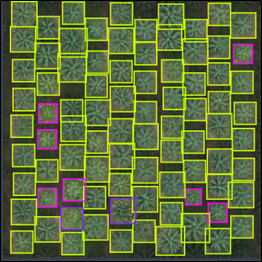
\includegraphics[width=6cm]{bab4/Gambar/Picture8.2.png} }}%
	\vspace{-0.2cm}
	%\rule{\columnwidth}{0.1pt}
	\captionsetup{justification=centering}
	\caption{Data Citra Asli Data Sekunder (kiri: original; kanan: tampak dengan \textit{bounding box}) }\label{img:Data-Citra-Asli-Data-Sekunder}
\end{figure}
%%%%%%%%%%%%%%%%%%%%%%%%%% GAMBAR %%%%%%%%%%%%%%%%%%%%%%%%%%%%%%

%%%%%%%%%%%%%%%%%%%%%%%TABEL SEDERHANA%%%%%%%%%%%%%%%%%%%%%%%%%
\begin{singlespace}
	\begin{table}[H]
		\centering
		\caption{Hasil Proses Augmentasi Citra Dataset Sekunder}
		\label{tbl:Hasil-Proses-Augmentasi-Citra-Dataset-Sekunder}
		\begin{tabular}{|m{3cm}|m{3cm}|m{6cm}|}
			\hline
			\rowcolor[HTML]{D9D9D9} 
			Augmentasi & Deskripsi                                                                & Citra Hasil Augmentasi \\ \hline
			
			
			Crop & 0\% Minimum Zoom,\newline 40\% Maximum Zoom & 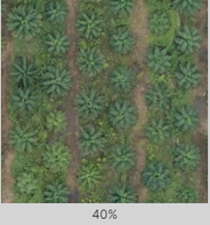
\includegraphics[width=0.4\columnwidth]{bab4/Gambar/tbl-5-pic1.png}\\ \hline
			
			Rotation & Between -39$^{\circ}$ and +39$^{\circ}$ & 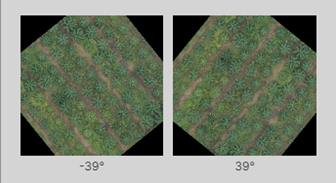
\includegraphics[width=0.4\columnwidth]{bab4/Gambar/tbl-5-pic2.png}\\ \hline
		\end{tabular}
	\end{table}
\end{singlespace}
%%%%%%%%%%%%%%%%%%%%%%%TABEL SEDERHANA%%%%%%%%%%%%%%%%%%%%%%%%%

%%%%%%%%%%%%%%%%%%%%%%%TABEL SEDERHANA%%%%%%%%%%%%%%%%%%%%%%%%%
\begin{singlespace}
	\begin{table}[H]
		\centering
		%\caption{Hasil Proses Augmentasi Citra Dataset Sekunder}
		%\label{tbl:Hasil-Proses-Augmentasi-Citra-Dataset-Sekunder}
		\begin{tabular}{|m{3cm}|m{3cm}|m{6cm}|}
			\hline
			\rowcolor[HTML]{D9D9D9} 
			Augmentasi & Deskripsi                                                                & Citra Hasil Augmentasi \\ \hline
			
			
			Hue & 0\% Between -30$^{\circ}$ and +30$^{\circ}$ & 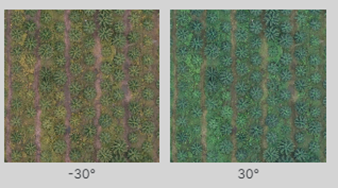
\includegraphics[width=0.4\columnwidth]{bab4/Gambar/tbl-5-pic3.png}\\ \hline
			
			Exposure & Between -17$^{\circ}$ and +17$^{\circ}$ & 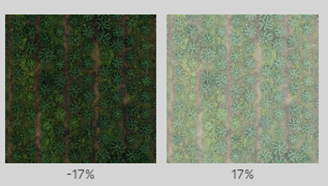
\includegraphics[width=0.4\columnwidth]{bab4/Gambar/tbl-5-pic4.png}\\ \hline
			
			Blur & Up to 2.5px & 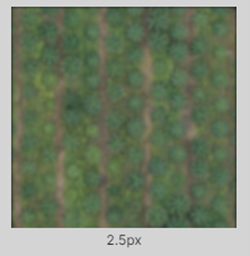
\includegraphics[width=0.4\columnwidth]{bab4/Gambar/tbl-5-pic5.png}\\ \hline
			
			Noise & Up to 2\% of pixels & 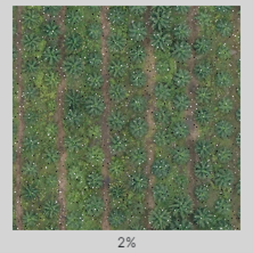
\includegraphics[width=0.4\columnwidth]{bab4/Gambar/tbl-5-pic6.png}\\ \hline
		\end{tabular}
	\end{table}
\end{singlespace}
%%%%%%%%%%%%%%%%%%%%%%%TABEL SEDERHANA%%%%%%%%%%%%%%%%%%%%%%%%%

%%%%%%%%%%%%%%%%%%%%%%%TABEL SEDERHANA%%%%%%%%%%%%%%%%%%%%%%%%%
\begin{singlespace}
	\begin{table}[H]
		\centering
		%\caption{Hasil Proses Augmentasi Citra Dataset Sekunder}
		%\label{tbl:Hasil-Proses-Augmentasi-Citra-Dataset-Sekunder}
		\begin{tabular}{|m{3cm}|m{3cm}|m{6cm}|}
			\hline
			\rowcolor[HTML]{D9D9D9} 
			Augmentasi & Deskripsi                                                                & Citra Hasil Augmentasi \\ \hline
			
			
			Mosaic & Applied & 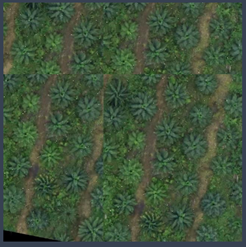
\includegraphics[width=0.4\columnwidth]{bab4/Gambar/tbl-5-pic7.png}\\ \hline
			
		\end{tabular}
	\end{table}
\end{singlespace}
%%%%%%%%%%%%%%%%%%%%%%%TABEL SEDERHANA%%%%%%%%%%%%%%%%%%%%%%%%%

Proses augmentasi dengan menambahkan 3987 citra tersimpan pada layanan roboflow yang digunakan citra untuk komputasi, yang terbagi untuk data pelatihan, validasi, dan pengujian dengan model CNN. Selanjutnya, untuk pembentukan dataset otomatis dengan memberikan anotasi atau pemberian label kelas secara otomatis pada objek di dalam citra dataset primer. Hal ini merupakan salah satu kebaruan pada penelitian ini dan proses tersebut dijelaskan pada sub bab \ref{sec:membangun-data}.

\subsection{Membersihkan Data}
\hspace{1,2cm}
Proses pada tahap membersihkan data dilakukan dengan memvalidasi data citra yang ditangkap pada dataset primer yang tidak dapat digunakan sebagai dataset. Proses ini dilakukan dengan validasi satu persatu dataset citra yang ditangkap oleh drone. Citra yang tidak digunakan merupakan citra yang ditangkap oleh drone tidak berada posisi yang tegak dari atas, tidak diambil dari sisi samping dari kamera drone dan tangkapan citra yang tidak terdapat pohon kelapa sawit. Terdapat 26 citra yang tidak dapat digunakan pada dataset primer sebagai citra untuk proses membangun data atau melakukan proses anotasi otomatis, seperti pada Gambar \ref{img:Data-Citra-Primer-Yang-Tidak-Digunakan}.

%%%%%%%%%%%%%%%%%%%%%%%%%% GAMBAR %%%%%%%%%%%%%%%%%%%%%%%%%%%%%%
\begin{figure}[H]
	\vspace{-0.1cm}
	%\rule{\columnwidth}{0.1pt}
	%\begin{center}
	%	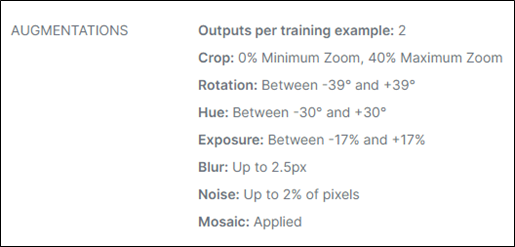
\includegraphics[width=1\columnwidth]{bab4/Gambar/Picture7.png}
	%\end{center}
	\centering
	\subfloat{{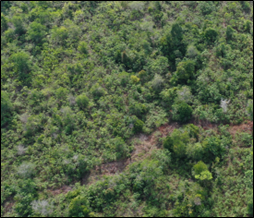
\includegraphics[width=6cm]{bab4/Gambar/Picture9.1.png} }}%
	\qquad
	\subfloat{{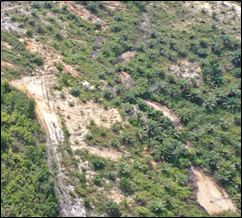
\includegraphics[width=6cm]{bab4/Gambar/Picture9.2.png} }}%
	\vspace{-0.2cm}
	%\rule{\columnwidth}{0.1pt}
	\captionsetup{justification=centering}
	\caption{Data Citra Primer yang tidak Digunakan (kiri: tidak terdapat pohon kelapa sawit; kanan: tampak area yang tidak tangkapan dari atas) }\label{img:Data-Citra-Primer-Yang-Tidak-Digunakan}
\end{figure}
%%%%%%%%%%%%%%%%%%%%%%%%%% GAMBAR %%%%%%%%%%%%%%%%%%%%%%%%%%%%%%

\subsection{Membangun Data}
\label{sec:membangun-data}
\hspace{1,2cm}
Proses anotasi otomatis merupakan pembentukan dataset berbasis OBIA. Proses anotasi ini digunakan dari data citra primer area studi Universitas Gunadarma di PPU, Kalimantan yaitu sebanyak 205 citra. Hasil dari 205 citra yang telah berhasil dideteksi sebagai objek pohon kelapa sawit ditampilkan dengan adanya \textit{bounding box} yang digunakan sebagai dataset untuk pelatihan dan pengujian model. Keluaran atau \textit{output} dari proses pembentukan dataset ini adalah citra yang dapat dideteksi objek di dalamnya sebagai pohon kelapa sawit yang dinyatakan dengan adanya \textit{bounding box} pada setiap objek yang terdeteksi yang memiliki data kelas, koordinat citra (x, y), dan \textit{width}, \textit{height} yang tersimpan dalam file dengan ekstensi *.txt.

Berdasarkan metode yang digunakan pada pembahasan bab 3 subbab \ref{sec:Deskripsi-Dataset-dan-Pemilihan-Data}, hal yang dilakukan pertama adalah menyiapkan pengumpulan data dalam satu folder yang sama. Data citra yang digunakan berupa 205 citra yang diambil oleh drone dari ketinggian 100 m dari permukaan tanah. Dalam penelitian ini, digunakan \textit{tools} atau peralatan berupa aplikasi \textit{jupyter notebook} untuk menuliskan kode program dan berbagi file dan berjalan di local komputer yang dijalankan pada web browser. Perintah yang digunakan dengan menggunakan \textit{command prompt} untuk mengaktifkan \textit{jupyter notebook}. Setelah berhasil aktif, maka diarahkan ke halaman homepage browser, dan dapat digunakan sebagai \textit{tools} untuk proses anotasi otomatis, seperti pada Gambar \ref{img:Home-Page-Jupyteer-Notebook}.

%%%%%%%%%%%%%%%%%%%%%%%%%% GAMBAR %%%%%%%%%%%%%%%%%%%%%%%%%%%%%%
\begin{figure}[H]
	\vspace{-0.1cm}
	\rule{\columnwidth}{0.1pt}
	\begin{center}
		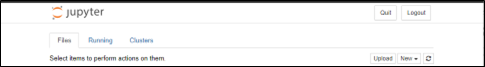
\includegraphics[width=1\columnwidth]{bab4/Gambar/Picture10.png}
	\end{center}
	\vspace{-0.2cm}
	%\rule{\columnwidth}{0.1pt}
	\captionsetup{justification=centering}
	\caption{\textit{Home Page} Jupyter Notebook}\label{img:Home-Page-Jupyteer-Notebook}
\end{figure}
%%%%%%%%%%%%%%%%%%%%%%%%%% GAMBAR %%%%%%%%%%%%%%%%%%%%%%%%%%%%%%

\subsection{Membuat Template}
\label{sec:Membuat-Template}
\hspace{1,2cm}
Tahap berikutnya dalam penelitian ini adalah membuat beberapa contoh gambar atau citra yang dijadikan sebagai template. Data citra yang digunakan berdimensi 5472 x 3078, maka pada jupyter notebook ditampilkan terlebih dahulu data citra untuk dapat ditampilkan citra yang digunakan untuk membuat template awal dengan sebuah fungsi. Data citra yang digunakan sebagai template seperti pada Gambar \ref{img:Data-Citra-Untuk-Membuat-Template}. 

%%%%%%%%%%%%%%%%%%%%%%%%%% GAMBAR %%%%%%%%%%%%%%%%%%%%%%%%%%%%%%
\begin{figure}[H]
	\vspace{-0.1cm}
	\rule{\columnwidth}{0.1pt}
	\begin{center}
		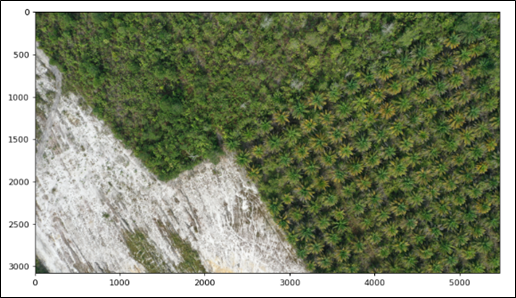
\includegraphics[width=1\columnwidth]{bab4/Gambar/Picture11.png}
	\end{center}
	\vspace{-0.2cm}
	%\rule{\columnwidth}{0.1pt}
	\captionsetup{justification=centering}
	\caption{Data citra untuk membuat template (5472 x 3078)}\label{img:Data-Citra-Untuk-Membuat-Template}
\end{figure}
%%%%%%%%%%%%%%%%%%%%%%%%%% GAMBAR %%%%%%%%%%%%%%%%%%%%%%%%%%%%%%

Dalam memudahkan pembuatan template gambar (objek kelapa sawit) digunakan fungsi \textit{onClick} untuk dapat menentukan beberapa titik tengah dari lokasi objek pohon kelapa sawit pada data citra. Dalam penelitian ini, digunakan 10 titik sebagai template objek. Titik yang dipilih merupakan objek citra pohon kelapa sawit yang ditandai dengan titik tengah merah yang berukuran 12 x 12 berdasarkan radius dari titik tengah yang telah ditentukan, seperti pada Gambar \ref{img:Membuat-Template-Yang-Ditandai}.

%%%%%%%%%%%%%%%%%%%%%%%%%% GAMBAR %%%%%%%%%%%%%%%%%%%%%%%%%%%%%%
\begin{figure}[H]
	\vspace{-0.1cm}
	\rule{\columnwidth}{0.1pt}
	\begin{center}
		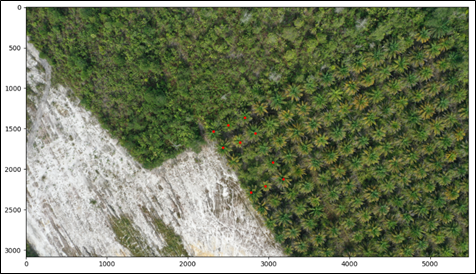
\includegraphics[width=1\columnwidth]{bab4/Gambar/Picture12.png}
	\end{center}
	\vspace{-0.2cm}
	%\rule{\columnwidth}{0.1pt}
	\captionsetup{justification=centering}
	\caption{Membuat Template yang Ditandai dengan Titik Objek Pohon Kelapa Sawit}\label{img:Membuat-Template-Yang-Ditandai}
\end{figure}
%%%%%%%%%%%%%%%%%%%%%%%%%% GAMBAR %%%%%%%%%%%%%%%%%%%%%%%%%%%%%%

Data citra berhasil ditampilkan dan ditandai dengan titik tengah merah untuk dijadikan sebagai template. Dalam pembuatan template ini, objek pohon kelapa sawit yang telah diberi titik dengan berwarna merah menjadi citra yang berukuran atau berdimensi 12 x 12 dari gambar asli. Citra tersebut ditampilkan dengan memiliki id dari 0 hingga 9 karena menggunakan array yang dimulai dari 0. Hal ini digunakan untuk dapat memudahkan penyesuaian titik tengah, jika terdapat titik yang tidak berada ditengah template yang diproses pada subbab 4.2.3.2. Gambar \ref{img:Citra-Template-Dari-Objek-Dari-Pohon-Kelapa-Sawit} hasil citra yang dijadikan sebagai template. 

%%%%%%%%%%%%%%%%%%%%%%%%%% GAMBAR %%%%%%%%%%%%%%%%%%%%%%%%%%%%%%
\begin{figure}[H]
	\vspace{-0.1cm}
	\rule{\columnwidth}{0.1pt}
	\begin{center}
		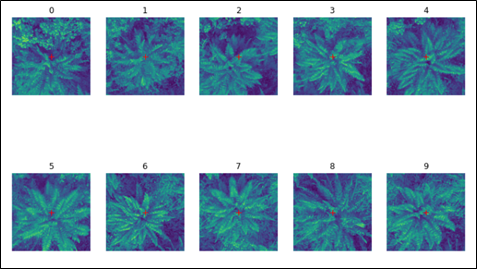
\includegraphics[width=1\columnwidth]{bab4/Gambar/Picture13.png}
	\end{center}
	\vspace{-0.2cm}
	%\rule{\columnwidth}{0.1pt}
	\captionsetup{justification=centering}
	\caption{Citra Template dari Objek Pohon Kelapa Sawit}\label{img:Citra-Template-Dari-Objek-Dari-Pohon-Kelapa-Sawit}
\end{figure}
%%%%%%%%%%%%%%%%%%%%%%%%%% GAMBAR %%%%%%%%%%%%%%%%%%%%%%%%%%%%%%

\subsubsection{Menyesuaikan Template}
\hspace{1,2cm}
Pada tahap ini, menyesuaikan template yang sudah tampak seperti pada gambar 4.10. Penyesuaian template adalah menyesuaikan titik tengah pada citra objek pohon kelapa sawit, jika titik tengah tidak berada pada tengah objek di citra tersebut. Penyesuaian ini dapat dilakukan dengan fungsi yang diterapkan, dan titik dapat dikoreksi dengan bergeser ke atas, bawah, kiri atau kanan dengan sebuah fungsi. Misalnya, pada id 2, titik tengah dari citra template tersebut yang ditandai dengan titik merah tidak berada di tengah, maka dapat digunakan fungsi turun (ke bawa) agar titik tersebut berada di tengah pohon kelapa sawit. Dalam penelitian ini dilakukan dengan 2 piksel setiap satu fungsi yang dijalankan untuk menggeser titik ke atas, bawah, kiri, atau kanan. Hasil koreksi dari menyesuaikan template untuk ID 2 ditampilkan pada Gambar \ref{img:Menyesuaikan-Template-Pada-ID-2}.

%%%%%%%%%%%%%%%%%%%%%%%%%% GAMBAR %%%%%%%%%%%%%%%%%%%%%%%%%%%%%%
\begin{figure}[H]
	\vspace{-0.1cm}
	\rule{\columnwidth}{0.1pt}
	\begin{center}
		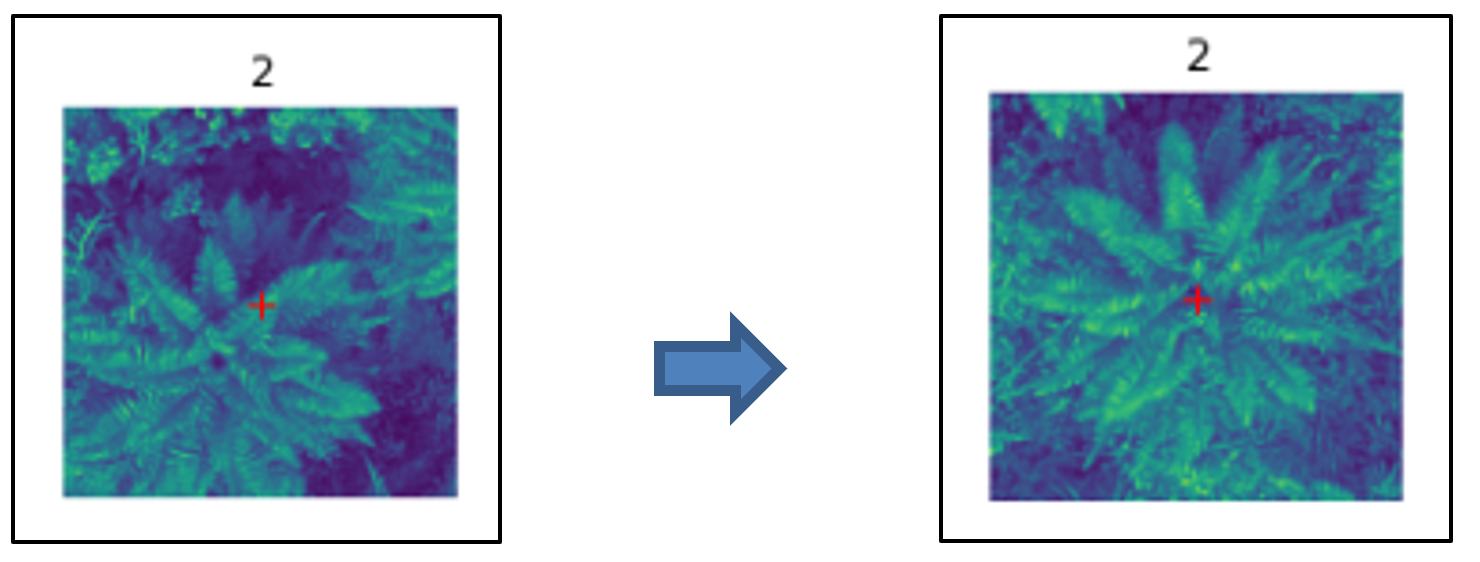
\includegraphics[width=1\columnwidth]{bab4/Gambar/Picture14.png}
	\end{center}
	\vspace{-0.2cm}
	%\rule{\columnwidth}{0.1pt}
	\captionsetup{justification=centering}
	\caption{Menyesuaikan Template pada ID 2}\label{img:Menyesuaikan-Template-Pada-ID-2}
\end{figure}
%%%%%%%%%%%%%%%%%%%%%%%%%% GAMBAR %%%%%%%%%%%%%%%%%%%%%%%%%%%%%%

\subsubsection{Evaluasi Korelasi diantara Template}
\hspace{1,2cm}
Ketika proses penyesuaian template selesai, maka pada tahap berikutnya adalah mengevaluasi korelasi antar template yang telah dibuat. Masing-masing template awal dibuat sebanyak 10 citra yang menunjukkan objek pohon kelapa sawit dengan dimensi 12 x 12. Dimensi 12 x 12 digunakan agar citra objek pohon kelapa sawit dapat terlihat lebih jelas yang menadakan 1 (satu) objek pohon kelapa sawit yang dipilih sebagai template. Berdasarkan perhitungan yang dilakukan pada persamaan 6 - 9 pada sub bab 3.3.3.3 didapatkan hasil korelasi diantara template dan waktu yang dibutuhkan untuk mengkalkulasi korelasi template tersebut pada Tabel \ref{tbl:Hasil-Rerata-Korelasi-dan-Waktu-Yang-Dibutuhkan}.

%%%%%%%%%%%%%%%%%%%%%%%TABEL SEDERHANA%%%%%%%%%%%%%%%%%%%%%%%%%
\begin{singlespace}
	\begin{table}[H]
		\centering
		\caption{Hasil Rerata Korelasi dan Waktu yang Dibutuhkan}
		\label{tbl:Hasil-Rerata-Korelasi-dan-Waktu-Yang-Dibutuhkan}
		\begin{tabular}{|p{8cm}|p{4cm}|}
			\hline
			\rowcolor[HTML]{D9D9D9} 
			Deskripsi                                 & Nilai \\ \hline
			Evaluasi korlasi diantara template        & 0.16  \\ \hline
			Waktu yang dibuthkan untuk menghitung (d) & 57    \\ \hline
		\end{tabular}
	\end{table}
\end{singlespace}
%%%%%%%%%%%%%%%%%%%%%%%TABEL SEDERHANA%%%%%%%%%%%%%%%%%%%%%%%%%

Berdasarkan Tabel \ref{tbl:Hasil-Rerata-Korelasi-dan-Waktu-Yang-Dibutuhkan}. terlihat bahwa waktu yang dibutuhkan untuk menghitung nilai rata-rata korelasi antar template membutuhkan waktu sebanyak 57 detik, dan nilai korelasi citra dihasilkan sebesar 0.16. Hal ini menunjukkan nila ikorelasi citra baik, karena nilai korelasi berada di rentang -1 sampai + 1. Jika nilai mendekati 1, maka nilai ini sebagai ambang batas untuk digunakan dalam metode atau algoritma \textit{template matching} untuk mendeteksi keberadaan objek kelapa sawit pada citra yang dapat diberikan anotasi atau label pohon kelapa sawit untuk dijadikan dataset.

\subsubsection{Penambahan Template}
\hspace{1,2cm}
Nilai korelasi antar template sudah diketahui, Langkah selanjutnya dilakukan menambahkan template dari 10 citra yang sudah dimiliki sebagai template. Hal ini digunakan untuk menambahkan data citra yang diproses pada \textit{template matching}, sehingga metode dapat digunakan dengan mengenali berbagai data citra sebagai template bahwa citra tersebut adalah objek pohon kelapa sawit. 

Pada penambahan template ini digunakan rotasi sebesar 30$^{\circ}$ (tiga puluh derajat), yang dimana setiap 1 gambar sebanyak 4 (empat kali) dirotasi sebesar 30$^{\circ}$. Hasil citra template yang sudah di rotasi seperti pada Gambar \ref{img:Hasil-Rotasi-30}. 

%%%%%%%%%%%%%%%%%%%%%%%%%% GAMBAR %%%%%%%%%%%%%%%%%%%%%%%%%%%%%%
\begin{figure}[H]
	\vspace{-0.1cm}
	\rule{\columnwidth}{0.1pt}
	\begin{center}
		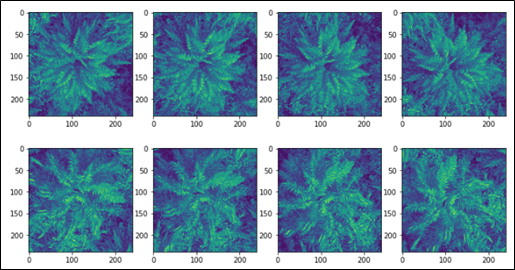
\includegraphics[width=1\columnwidth]{bab4/Gambar/Picture15.png}
	\end{center}
	\vspace{-0.2cm}
	%\rule{\columnwidth}{0.1pt}
	\captionsetup{justification=centering}
	\caption{Hasil Rotasi 30$^{\circ}$ pada Citra template}\label{img:Hasil-Rotasi-30}
\end{figure}
%%%%%%%%%%%%%%%%%%%%%%%%%% GAMBAR %%%%%%%%%%%%%%%%%%%%%%%%%%%%%%

Proses untuk mendapatkan citra yang di rotasi untuk 10 (sepuluh) citra template tampak seperti pada Tabel \ref{tbl:Waktu-Yang-Dibutuhkan-Untuk-Rotasi}. 

%%%%%%%%%%%%%%%%%%%%%%%TABEL SEDERHANA%%%%%%%%%%%%%%%%%%%%%%%%%
\begin{singlespace}
	\begin{table}[H]
		\centering
		\caption{Waktu yang Dibutuhkan untuk Rotasi}
		\label{tbl:Waktu-Yang-Dibutuhkan-Untuk-Rotasi}
		\begin{tabular}{|p{8cm}|p{4cm}|}
			\hline
			\rowcolor[HTML]{D9D9D9} 
			Deskripsi                                  & Nilai \\ \hline
			Waktu yang dibutuhkan untuk rotasi (detik) & 8 \\ \hline
		\end{tabular}
	\end{table}
\end{singlespace}
%%%%%%%%%%%%%%%%%%%%%%%TABEL SEDERHANA%%%%%%%%%%%%%%%%%%%%%%%%%

\subsubsection{Menjalankan Template Matching}
\hspace{1,2cm}
Pada tahap ini dilakukan match template yaitu anotasi secara otomatis dengan mendeteksi (klasifikasi) mengenali adanya objek pohon kelapa sawit pada citra. Citra utuh yang besar (gambar asli) dideteksi menjadi bagian-bagian yang terdeteksi menjadi citra yang dikenali sebagai objek yang menjadi dataset. Gambar yang terdeteksi dengan \textit{template matching} ini dideteksi dengan lingkarran merah pada Gambar \ref{img:Objek-Yang-Terdeteksi-Untuk-Dataset}.

%%%%%%%%%%%%%%%%%%%%%%%%%% GAMBAR %%%%%%%%%%%%%%%%%%%%%%%%%%%%%%
\begin{figure}[H]
	\vspace{-0.1cm}
	\rule{\columnwidth}{0.1pt}
	\begin{center}
		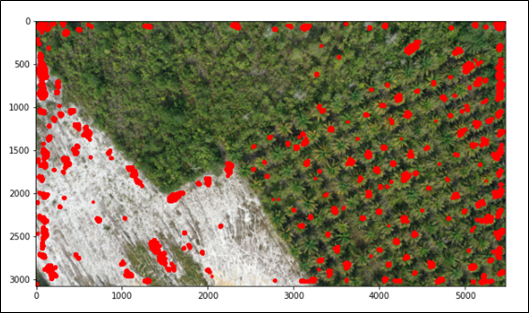
\includegraphics[width=1\columnwidth]{bab4/Gambar/Picture16.png}
	\end{center}
	\vspace{-0.2cm}
	%\rule{\columnwidth}{0.1pt}
	\captionsetup{justification=centering}
	\caption{Objek yang terdeteksi untuk Dataset dengan \textit{Template Matching}}\label{img:Objek-Yang-Terdeteksi-Untuk-Dataset}
\end{figure}
%%%%%%%%%%%%%%%%%%%%%%%%%% GAMBAR %%%%%%%%%%%%%%%%%%%%%%%%%%%%%%

Gambar \ref{img:Objek-Yang-Terdeteksi-Untuk-Dataset}. yang terdeteksi terlihat seperti adanya tumpang tindih atau mungkin tidak seperti pohon kelapa sawit yang merupakan dataset yang diharapkan, karena nilai ambang batas (\textit{threshold}) dibatasi pada nilai rata-rata nilai korelasi diantara template yang lebih rendah, sehingga ketika berada di atas nilai korelasi, maka terdeteksi sebagai citra yang cocok dengan template.

\subsubsection{Analisis Cluster dengan BIRCH}
\hspace{1,2cm}
Tahap ini dilakukan setelah berhasil dideteksi dengan menggunakan \textit{template matching}, selanjutnya dilakukan analisis cluster dengan algoritma BIRCH untuk mereduksi atau mencari nilai ambang batas dari citra yang tidak sesuai berdasarkan nilai mean r (korelasi). Pada BIRCH ini digunakan nilai ambang batas (\textit{threshold}) secara acak yang digunakan sebagai nilai ambang batas minimum yang dimasukkan ke dalam citra untuk dapat mendeteksi objek yang terdeteksi pohon kelapa sawit pada citra yang sudah dideteksi dengan \textit{template matching}. Nilai ambang batas (threshold) yang digunakan dalam penelitian ini adalah 0.5. Hasil objek yang terdeteksi sebagai pohon kelapa sawit pada citra untuk menjadi dataset ditampilkan dengan kotak batas (\textit{bounding box}) dengan kotak berwarna merah. Hal ini menujukkan bahwa kotak tersebut mendeteksi objek pohon kelapa sawit yang tampak seperti pada Gambar \ref{img:Hasil-Objek-Yang-Terdeteksi}.

%%%%%%%%%%%%%%%%%%%%%%%%%% GAMBAR %%%%%%%%%%%%%%%%%%%%%%%%%%%%%%
\begin{figure}[H]
	\vspace{-0.1cm}
	\rule{\columnwidth}{0.1pt}
	\begin{center}
		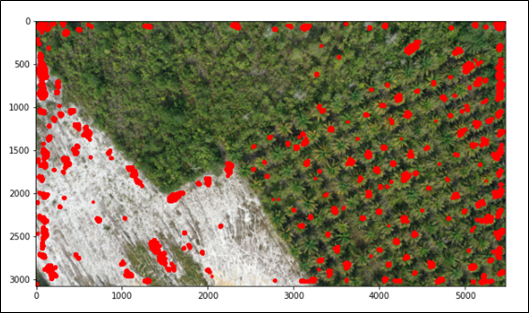
\includegraphics[width=1\columnwidth]{bab4/Gambar/Picture16.png}
	\end{center}
	\vspace{-0.2cm}
	%\rule{\columnwidth}{0.1pt}
	\captionsetup{justification=centering}
	\caption{Hasil objek yang terdeteksi untuk Dataset dengan algoritma BIRCH}\label{img:Hasil-Objek-Yang-Terdeteksi}
\end{figure}
%%%%%%%%%%%%%%%%%%%%%%%%%% GAMBAR %%%%%%%%%%%%%%%%%%%%%%%%%%%%%%

Berdasarkan Gambar \ref{img:Objek-Yang-Terdeteksi-Untuk-Dataset} diketahui template matching dari citra berhasil mendeteksi objek untuk dataset, namun masih terjadi tumpang tindih atau overlapping dan berdasarkan hasil dari algoritma BIRCH pada Gambar \ref{img:Hasil-Objek-Yang-Terdeteksi}., dihasilkan pengurangan nilai dan terdeteksi objek pohon kelapa sawit pada citra. Hasil waktu yang digunakan untuk mendeteksi objek sebagai dataset ditunjukkan pada Tabel \ref{tbl:Hasil-Waktu-Yang-Dibutuhkan-Untuk-Deteksi-Objek-Sebagai-Dataset}.

%%%%%%%%%%%%%%%%%%%%%%%TABEL SEDERHANA%%%%%%%%%%%%%%%%%%%%%%%%%
\begin{singlespace}
	\begin{table}[H]
		\centering
		\caption{Hasil Waktu yang Dibutuhkan untuk Deteksi Objek sebagai Dataset}
		\label{tbl:Hasil-Waktu-Yang-Dibutuhkan-Untuk-Deteksi-Objek-Sebagai-Dataset}
		\begin{tabular}{|m{5cm}|m{3cm}|m{4cm}|}
			\hline
			\rowcolor[HTML]{D9D9D9} 
			Deskripsi                                    & Waktu (detik) & Jumlah yang Terdeteksi \\ \hline
			Waktu yang dibutuhkan pada Template Matching & 334              & 463                    \\ \hline
			Waktu yang dibutuhkan pada BIRCH             & 24               & 148                    \\ \hline
		\end{tabular}
	\end{table}
\end{singlespace}
%%%%%%%%%%%%%%%%%%%%%%%TABEL SEDERHANA%%%%%%%%%%%%%%%%%%%%%%%%%

Berdasarkan hasil Tabel \ref{tbl:Hasil-Waktu-Yang-Dibutuhkan-Untuk-Deteksi-Objek-Sebagai-Dataset}. diketahui bahwa \textit{template matching} membutuhkan waktu 334 detik untuk berhasil mendeteksi 463 objek, sedangkan dengan BIRCH membutuhkan waktu 24 detik dan berhasil direduksi untuk menemukan nilai ambang batas yang baik menjadi 148 yang terdeteksi sesuai dengan nilai yang telah ditentukan. 

\subsubsection{Menjalankan Auto-Annotate Datasets}
\hspace{1,2cm}
Proses dengan \textit{template matching} dan BIRCH berhasil dideteksi objek pada citra yang ditampilkan dengan \textit{bounding box}. Tahap selanjutnya menjalankan anotasi otomatis. Proses ini mengambil data citra sebanyak 205 citra dari data primer yang berada dalam 1 folder, kemudian dijalankan proses tersebut. Proses ini mendeteksi objek yang sesuai sebagai pohon kelapa sawit pada citra, sehingga dapat dikenali dan diperoleh kelas, koordinat x, koordinat y, \textit{width}, \textit{height} disimpan dalam file berekstensi *.txt (sesuai nama file citra). File merupakan hasil dari proses anotasi dataset yang berisi kelas, koordinat x, koordinat y, \textit{width}, \textit{height}.

Berdasarkan hasil anotasi otomatis membutuhkan waktu yang signifikan untuk membuat dataset dengan anotasi otomatis dari citra yang berjumlah 205. Waktu yang dibutuhkan proses ini seperti terlihat pada Tabel 4.9.

%%%%%%%%%%%%%%%%%%%%%%%TABEL SEDERHANA%%%%%%%%%%%%%%%%%%%%%%%%%
\begin{singlespace}
	\begin{table}[H]
		\centering
		\caption{Hasil Waktu Yang Dibutuhkan untuk Anotasi Otomatis}
		\label{tbl:Hasil-Waktu-Yang-Dibutuhkan-Untuk-Anotasi-Otomatis}
		\begin{tabular}{|m{10cm}|m{2cm}}
			\hline
			\rowcolor[HTML]{D9D9D9} 
			Deskripsi                                            & Waktu (mm:dd) \\ \hline
			Waktu yang dibutuhkan untuk Anotasi Otomatis Dataset & 30:24         \\ \hline
		\end{tabular}
	\end{table}
\end{singlespace}
%%%%%%%%%%%%%%%%%%%%%%%TABEL SEDERHANA%%%%%%%%%%%%%%%%%%%%%%%%%

Berikut ini adalah contoh hasil anotasi otomatis pada file berekstensi *.txt yang berisi kelas, koordinat x, koordinat y, width, dan height terlihat pada Gambar 4.18.

%%%%%%%%%%%%%%%%%%%%%%%%%% GAMBAR %%%%%%%%%%%%%%%%%%%%%%%%%%%%%%
\begin{figure}[H]
	\vspace{-0.1cm}
	%\rule{\columnwidth}{0.1pt}
	\begin{center}
		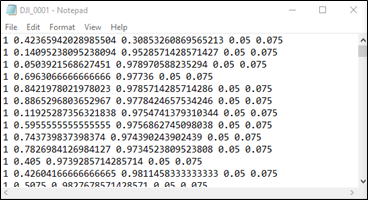
\includegraphics[width=0.6\columnwidth]{bab4/Gambar/Picture18.1.png}
		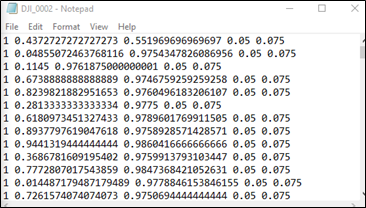
\includegraphics[width=0.6\columnwidth]{bab4/Gambar/Picture18.2.png}
	\end{center}
	\vspace{-0.2cm}
	%\rule{\columnwidth}{0.1pt}
	\captionsetup{justification=centering}
	\caption{Hasil Anotasi Otomatis dalam format file *.txt}\label{img:Hasil-Anotasi-Otomatis}
\end{figure}
%%%%%%%%%%%%%%%%%%%%%%%%%% GAMBAR %%%%%%%%%%%%%%%%%%%%%%%%%%%%%%

Pada Gambar \ref{img:Hasil-Anotasi-Otomatis}. terdapat 5 bilangan berurutan, nilai ke-1 menunjukkan bilangan yang sama, untuk digunakan sebagai kelas yang terdeteksi yaitu kelas 'oil palm', untuk barisan ke-2, ke-3, ke-4, dan ke-5 masing-masing menunjukkan koordinat x, koordinat y, lebar dan tinggi. Lebar dan tinggi dapat terlihat sama, karena dataset memiliki karakteristik dimensi ukuran citra yang sama.

Setelah itu, pada penelitian ini dilakukan pengujian dengan 10 citra yang dapat dilihat pada Tabel \ref{tbl:Pengujian-Dengan-10-Citra-Dataset-Primer}.

%%%%%%%%%%%%%%%%%%%%%%%TABEL SEDERHANA%%%%%%%%%%%%%%%%%%%%%%%%%
\begin{singlespace}
	\begin{table}[H]
		\centering
		\caption{Pengujian dengan 10 Citra Dataset Primer}
		\label{tbl:Pengujian-Dengan-10-Citra-Dataset-Primer}
		%\begin{tabular}{|m{0.5cm}|m{2cm}|m{3cm}|m{3cm}|m{3cm}|}
		\begin{tabular}{|m{0.5cm}m{1cm}m{3cm}m{3cm}|m{3cm}|}
			\hline
		
			\multicolumn{1}{|m{0.5cm}|}{No} & \multicolumn{1}{m{2cm}|}{ID\_Image} & \multicolumn{1}{m{3cm}|}{Jumlah objek Pohon yang Asli} & Jumlah objek Pohon yang terdeteksi & Hasil \% Terdeteksi \\ \hline
			
			\multicolumn{1}{|m{0.5cm}|}{1}  & \multicolumn{1}{m{2cm}|}{ID 1}      & \multicolumn{1}{m{3cm}|}{253}                          & 233                                & 92,1\%              \\ \hline
			
			\multicolumn{1}{|m{0.5cm}|}{2}  & \multicolumn{1}{m{2cm}|}{ID 2}      & \multicolumn{1}{m{3cm}|}{273}                          & 250                                & 91,6\%              \\ \hline
			
			\multicolumn{1}{|m{0.5cm}|}{3}  & \multicolumn{1}{m{2cm}|}{ID 3}      & \multicolumn{1}{m{3cm}|}{157}                          & 142                                & 90,4\%              \\ \hline
			
			\multicolumn{1}{|m{0.5cm}|}{4}  & \multicolumn{1}{m{2cm}|}{ID 4}      & \multicolumn{1}{m{3cm}|}{167}                          & 148                                & 88,6\%              \\ \hline
			
			\multicolumn{1}{|m{0.5cm}|}{5}  & \multicolumn{1}{m{2cm}|}{ID 5}      & \multicolumn{1}{m{3cm}|}{113}                          & 101                                & 89,4\%              \\ \hline
			
			\multicolumn{1}{|m{0.5cm}|}{6}  & \multicolumn{1}{m{2cm}|}{ID 6}      & \multicolumn{1}{m{3cm}|}{110}                          & 97                                 & 88,2\%              \\ \hline
			
			\multicolumn{1}{|m{0.5cm}|}{7}  & \multicolumn{1}{m{2cm}|}{ID 7}      & \multicolumn{1}{m{3cm}|}{84}                           & 75                                 & 89,3\%              \\ \hline
			
			\multicolumn{1}{|m{0.5cm}|}{8}  & \multicolumn{1}{m{2cm}|}{ID 8}      & \multicolumn{1}{m{3cm}|}{138}                          & 121                                & 87,7\%              \\ \hline
			
			\multicolumn{1}{|m{0.5cm}|}{9}  & \multicolumn{1}{m{2cm}|}{ID 9}      & \multicolumn{1}{m{3cm}|}{160}                          & 144                                & 90,0\%              \\ \hline
			
			\multicolumn{1}{|m{0.5cm}|}{10} & \multicolumn{1}{m{2cm}|}{ID 10}     & \multicolumn{1}{m{3cm}|}{210}                          & 186                                & 88,6\%              \\ \hline
		
			\multicolumn{4}{|l|}{\textbf{Rata-Rata}}                                                                                                           & \textbf{89,9\%}     \\ \hline
		\end{tabular}
	\end{table}
\end{singlespace}
%%%%%%%%%%%%%%%%%%%%%%%TABEL SEDERHANA%%%%%%%%%%%%%%%%%%%%%%%%%

Berdasarkan hasil pengujian terhadap 10 citra dari hasil pada Tabel \ref{tbl:Pengujian-Dengan-10-Citra-Dataset-Primer} didapatkan rata-rata akurasi yang terdeteksi pada penelitian ini sebesar 89.90\% dengan menggunakan metode \textit{template matching} dan algoritma BIRCH. Hal ini menunjukkan hal penting yang signifikan yang harus dilakukan dalam proses anotasi otomatis yang dapat digunakan untuk memberikan deteksi gambar yang lebih akurat dan lebih cepat.

Setelah dilakukan pengujian dan juga dilakukan anotasi otomatis dari citra dan deteksi objek pohon kelapa sawit, maka citra yang tersimpan pada folder di local komputer beserta format file *.txt yang merupakan dataset. Hasil tersebut seperti pada Gambar \ref{img:Gambar-Dan-File.txt}

%%%%%%%%%%%%%%%%%%%%%%%%%% GAMBAR %%%%%%%%%%%%%%%%%%%%%%%%%%%%%%
\begin{figure}[H]
	\vspace{-0.1cm}
	%\rule{\columnwidth}{0.1pt}
	\begin{center}
		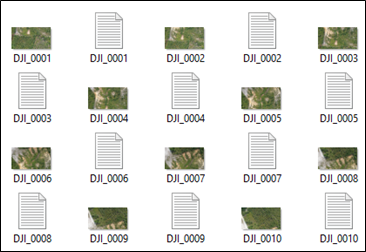
\includegraphics[width=0.8\columnwidth]{bab4/Gambar/Picture19.png}
	\end{center}
	\vspace{-0.2cm}
	%\rule{\columnwidth}{0.1pt}
	\captionsetup{justification=centering}
	\caption{Gambar dan File *.txt}\label{img:Gambar-Dan-File.txt}
\end{figure}
%%%%%%%%%%%%%%%%%%%%%%%%%% GAMBAR %%%%%%%%%%%%%%%%%%%%%%%%%%%%%%

\subsubsection{Integrasi Data}
\hspace{1,2cm}
Proses integrasi data dilakukan untuk menggabungkan atau menyatukan dua dataset, yaitu dataset primer dan sekunder ke dalam satu sumber. Dataset sekunder digunakan layanan roboflow untuk menampung data yang sudah tersimpan pada layanan tersebut. Selanjutnya, hasil dari pembangunan dataset dengan anotasi atau pelabelan otomatis yang telah dilakukan, maka diunggah data citra dan file *.txt. 

%%%%%%%%%%%%%%%%%%%%%%%%%% GAMBAR %%%%%%%%%%%%%%%%%%%%%%%%%%%%%%
\begin{figure}[H]
	\vspace{-0.1cm}
	%\rule{\columnwidth}{0.1pt}
	\begin{center}
		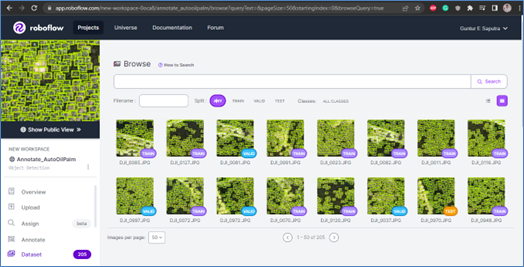
\includegraphics[width=1\columnwidth]{bab4/Gambar/Picture20.png}
	\end{center}
	\vspace{-0.2cm}
	%\rule{\columnwidth}{0.1pt}
	\captionsetup{justification=centering}
	\caption{Dataset Data Primer Drone di Roboflow}\label{img:Dataset-Data-Primer-Drone-di-Roboflow}
\end{figure}
%%%%%%%%%%%%%%%%%%%%%%%%%% GAMBAR %%%%%%%%%%%%%%%%%%%%%%%%%%%%%%

Pada Gambar \ref{img:Dataset-Data-Primer-Drone-di-Roboflow} terlihat kumpulan gambar sebanyak 205 gambar yang menandakan bahwa dataset dari citra asli sebanyak 205 berhasil terunggah, dan satu citra dapat memiliki lebih dari objek pohon kelapa sawit dengen kelas 'oil palm' pada satu citra. 

Pada Gambar \ref{img:Dataset-Data-Primer-Drone-di-Roboflow} dan \ref{img:Banyaknya-Objek-Yang-Terdeteksi-Sebagai-Pohon-Kelapa} terlihat kotak pembatas atau yang dikenal dengan nama \textit{bounding box} yang berwarna hijau, hal ini menandakan objek yang terdeteksi sebagai dataset. Setiap 1 citra dataset primer memiliki jumlah \textit{bounding box} yang berbeda-beda karena tergantung hasil yang dideteksi, seperti pada Gambar \ref{img:Banyaknya-Objek-Yang-Terdeteksi-Sebagai-Pohon-Kelapa} terdapat 414 objek pohon kelapa sawit yang terdeteksi dalam anotasi atau label dari 1 citra. 

%%%%%%%%%%%%%%%%%%%%%%%%%% GAMBAR %%%%%%%%%%%%%%%%%%%%%%%%%%%%%%
\begin{figure}[H]
	\vspace{-0.1cm}
	%\rule{\columnwidth}{0.1pt}
	\begin{center}
		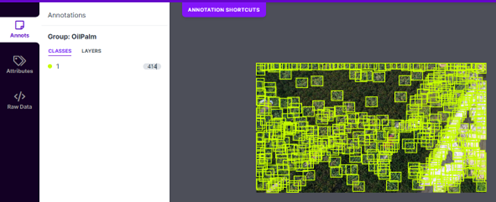
\includegraphics[width=1\columnwidth]{bab4/Gambar/Picture21.png}
	\end{center}
	\vspace{-0.2cm}
	%\rule{\columnwidth}{0.1pt}
	\captionsetup{justification=centering}
	\caption{Banyaknya Objek yang Terdeteksi sebagai Pohon Kelapa Sawit}\label{img:Banyaknya-Objek-Yang-Terdeteksi-Sebagai-Pohon-Kelapa}
\end{figure}
%%%%%%%%%%%%%%%%%%%%%%%%%% GAMBAR %%%%%%%%%%%%%%%%%%%%%%%%%%%%%%

Berdasarkan hasil yang telah dilakukan pada pembentukan dataset secara otomatis dengan pendekatan OBIA berhasil dilakukan, dan citra yang menjadi dataset primer dapat digunakan dan di integrasikan (digabungkan) dengan dataset sekunder untuk komputasi. 

\subsubsection{Format Data}
\hspace{1,2cm}
Pada proses ini dilakukan format data primer dan sekunder dengan menggunakan bantuan layanan roboflow sebelum dapat digunakan untuk citra komputasi yang dibagi menjadi dataset pelatihan, validasi, dan test.  Pada tahap ini menyesuaikan tipe data pada citra yaitu pada dataset primer dan sekunder sama-sama *.jpg, dan mengurangi dimensi dataset citra dengan melakukan resize citra menjadi 640 x 640, seperti pada Gambar \ref{img:Format-Data}.

%%%%%%%%%%%%%%%%%%%%%%%%%% GAMBAR %%%%%%%%%%%%%%%%%%%%%%%%%%%%%%
\begin{figure}[H]
	\vspace{-0.1cm}
	%\rule{\columnwidth}{0.1pt}
	\begin{center}
		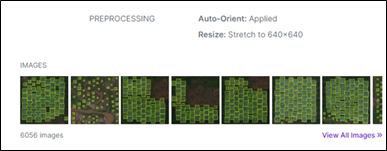
\includegraphics[width=1\columnwidth]{bab4/Gambar/Picture22.png}
	\end{center}
	\vspace{-0.2cm}
	%\rule{\columnwidth}{0.1pt}
	\captionsetup{justification=centering}
	\caption{Format Data}\label{img:Format-Data}
\end{figure}
%%%%%%%%%%%%%%%%%%%%%%%%%% GAMBAR %%%%%%%%%%%%%%%%%%%%%%%%%%%%%%

Ketika proses pada Gambar 4.22 sudah dilakukan, maka selanjutnya dataset yang telah sesuai dengan format data yang ditentukan dapat digunakan untuk citra komputasi. Dataset dipindahkan ke layanan Google Drive untuk kemudian dilakukan citra komputasi yang membagi data untuk data pelatihan, validasi dan pengujian sesuai dengan fold yang digunakan, yaitu sebanyak 5 fold (dengan nama dataset folds 0 sampai 4) seperti Gambar \ref{img:Dataset-Pada-Gdrive}.

%%%%%%%%%%%%%%%%%%%%%%%%%% GAMBAR %%%%%%%%%%%%%%%%%%%%%%%%%%%%%%
\begin{figure}[H]
	\vspace{-0.1cm}
	%\rule{\columnwidth}{0.1pt}
	\begin{center}
		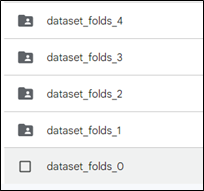
\includegraphics[width=0.4\columnwidth]{bab4/Gambar/Picture23.png}
	\end{center}
	\vspace{-0.2cm}
	%\rule{\columnwidth}{0.1pt}
	\captionsetup{justification=centering}
	\caption{Dataset pada layanan Google Drive}\label{img:Dataset-Pada-Gdrive}
\end{figure}
%%%%%%%%%%%%%%%%%%%%%%%%%% GAMBAR %%%%%%%%%%%%%%%%%%%%%%%%%%%%%%

\section{Citra untuk Komputasi}
\hspace{1,2cm}
Pada tahap ini citra gambar untuk komputasi merupakan kumpulan dari citra dataset primer dan sekunder. Jumlah dataset sebanyak 6056 data, yang terbagi ke dalam 78\% data pelatihan, 20\% data validasi dan 2\% data pengujian, seperti pada Tabel \ref{tbl:Dataset-Untuk-Komputasi}.

%%%%%%%%%%%%%%%%%%%%%%%TABEL SEDERHANA%%%%%%%%%%%%%%%%%%%%%%%%%
\begin{singlespace}
	\begin{table}[H]
		\centering
		\caption{Dataset untuk Komputasi}
		\label{tbl:Dataset-Untuk-Komputasi}
		\begin{tabular}{|m{5cm}|m{5cm}|}
			\hline
			\rowcolor[HTML]{D9D9D9} 
			Dataset   & Jumlah \\ \hline
			Pelatihan & 4744   \\ \hline
			Validasi  & 1187   \\ \hline
			Pengujian & 125    \\ \hline
		\end{tabular}
	\end{table}
\end{singlespace}
%%%%%%%%%%%%%%%%%%%%%%%TABEL SEDERHANA%%%%%%%%%%%%%%%%%%%%%%%%%

Dataset tersebut dikumpulkan atau digabungkan, serta dibagi menjadi 5 bagian. Karena pada proses pelatihan dan pengujian mengunakan teknik evaluasi K-Fold Cross-Validation. Berikut ini contoh citra yang digunakan dengan file *.txt yang berisi anotasi objek yang digunakan untuk dataset pelatihan, dataset validasi, dan dataset pengujian seperti tampak pada Gambar \ref{img:Contoh-Citra-Yang-Digunakan-Untuk-Komputasi}.

%%%%%%%%%%%%%%%%%%%%%%%%%% GAMBAR %%%%%%%%%%%%%%%%%%%%%%%%%%%%%%
\begin{figure}[H]
	\vspace{-0.1cm}
	%\rule{\columnwidth}{0.1pt}
	%\begin{center}
	%	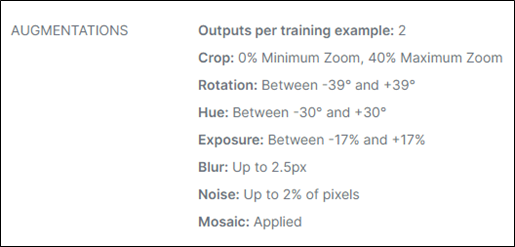
\includegraphics[width=1\columnwidth]{bab4/Gambar/Picture7.png}
	%\end{center}
	\centering
	
	\subfloat{{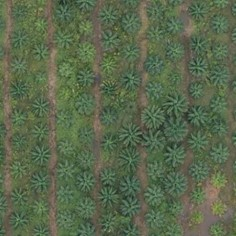
\includegraphics[width=6cm]{bab4/Gambar/Picture24.1.1.jpg} }}%
	\subfloat{{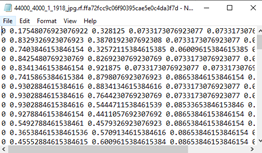
\includegraphics[width=5cm]{bab4/Gambar/Picture24.1.2.png} }}%
	\vspace{-0.2cm}\\
	(a)
	
	\subfloat{{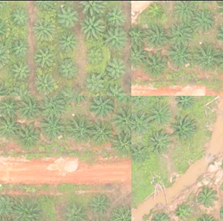
\includegraphics[width=6cm]{bab4/Gambar/Picture24.2.1.png} }}%
	\subfloat{{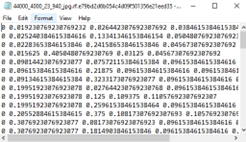
\includegraphics[width=5cm]{bab4/Gambar/Picture24.2.2.png} }}%
	\vspace{-0.2cm}\\
	(b)
	
	\subfloat{{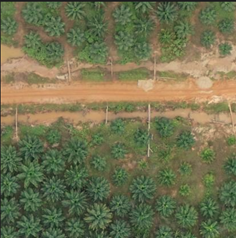
\includegraphics[width=6cm]{bab4/Gambar/Picture24.3.1.png} }}%
	\subfloat{{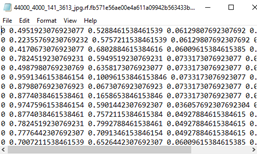
\includegraphics[width=5cm]{bab4/Gambar/Picture24.3.2.png} }}%
	\vspace{-0.2cm}\\
	(b)
	
	%\rule{\columnwidth}{0.1pt}
	\captionsetup{justification=centering}
	\caption{Contoh Citra yang digunakan untuk komputasi (a) Citra dataset pelatihan; (b) Citra dataset validasi; (c) Citra dataset pengujian;}\label{img:Contoh-Citra-Yang-Digunakan-Untuk-Komputasi}
\end{figure}
%%%%%%%%%%%%%%%%%%%%%%%%%% GAMBAR %%%%%%%%%%%%%%%%%%%%%%%%%%%%%%

\section{Pelatihan Model CNN}
\hspace{1,2cm}
Pada proses pelatihan ini dengan menggunakan model CNN pada YOLOv5, YOLOv6, dan YOLOv7 yang divalidasi dengan menggunakan K-Fold Cross-Validation, dimana semua bagian dataset dapat digunakan untuk pelatihan dan pengujian. Teknik ini digunakan untuk evaluasi performance dari model untuk mengurangi overfitting.  Pada penelitian ini menggunakan k = 5, dimana proses ini diulang sebanyak k = 5 kali. Setiap fold masing-masing terdiri dari data pelatihan yang merupakan gabungan dari data pelatihan sebanyak 4744 data dan 1187 validasi, untuk data test sebanyak 125 data citra. Setiap fold berisi data ini untuk dapat diketahui pada fold mana hasil model yang dilatih hasilnya lebih baik. Pada proses pelatihan ini data citr auntuk dataset dikonversi untuk data masukkan gambar pada proses pelatihan dengan menggunakan ukuran gambar yang diatur oleh YOLO, yaitu secara \textit{default} 640 x 640. Pada pelatihan model dan pengujian menggunakan parameter optimasi seperti pada Tabel \ref{tbl:Optimisasi-Parameter2}.

%%%%%%%%%%%%%%%%%%%%%%%TABEL SEDERHANA%%%%%%%%%%%%%%%%%%%%%%%%%
\begin{singlespace}
	\begin{table}[H]
		\centering
		\caption{Optimisasi Parameter}
		\label{tbl:Optimisasi-Parameter2}
		\begin{tabular}{|m{5cm}|m{5cm}|}
			\hline
			\rowcolor[HTML]{D9D9D9} 
			Parameter    & Nilai         \\ \hline
			lr0          & 0.01 (1E-2)   \\ \hline
			lrf          & 0.1           \\ \hline
			Momentum     & 0.937         \\ \hline
			Weight decay & 0.0005 (5e-4) \\ \hline
			Epoch        & 30            \\ \hline
			Batch size   & 16            \\ \hline
		\end{tabular}
	\end{table}
\end{singlespace}
%%%%%%%%%%%%%%%%%%%%%%%TABEL SEDERHANA%%%%%%%%%%%%%%%%%%%%%%%%%

Pada pelatihan menggunakan mesin pada Google Colab Pro dan DGX-A-100 yang dimiliki oleh Universitas Gunadarma. Mesin NVIDIA yang digunakan, seperti pada Tabel \ref{tbl:Sarana-Penelitian-Mesin-Nvidia}.


%%%%%%%%%%%%%%%%%%%%%%%TABEL SEDERHANA%%%%%%%%%%%%%%%%%%%%%%%%%
\begin{singlespace}
	\begin{table}[H]
		\centering
		\caption{Sarana Penelitian Mesin NVIDIA (Super Komputer)}
		\label{tbl:Sarana-Penelitian-Mesin-Nvidia}
		\begin{tabular}{|m{5cm}|m{5cm}|}
			\hline
			\rowcolor[HTML]{D9D9D9} 
			Mesin NVIDIA                    & Keterangan                       \\ \hline
			Google Colab Pro                & A-100-SXM4-40GB, 40536.1875 MB   \\ \hline
			DGX-A-100 Universitas Gunadarma & A-100-SXM4-40GB, 20096 MB        \\ \hline
		\end{tabular}
	\end{table}
\end{singlespace}
%%%%%%%%%%%%%%%%%%%%%%%TABEL SEDERHANA%%%%%%%%%%%%%%%%%%%%%%%%%

Pelatihan model CNN pada penelitian ini menggunakan validasi performance yang menghasilkan 4 hasil yang berbeda dengan menggunakan \textit{Precision}, \textit{Recall}, \textit{F1-Score}, dan \textit{best mean Average Precision} atau best mAP@0.5.

\subsection{Pelatihan Model CNN YOLOv5}
\hspace{1,2cm}
Pelatihan model pertama dilatih dengan menggunakan YOLOv5. Pada Tabel 4.13 hasil pelatihan model CNN dengan YOLOv5 dengan 30 epoch dan batch size 16 pada Google Colab Pro. Pada mesin DGX-A-100 milik Universitas Gunadarma dengan menggunakan batch size sebesar 16 tidak dapat dijalankan karena permasalahan \textit{suificient memory} (runs out memory) atau kehabisan shared virtual memori untuk dapat digunakan, sehingga menggunakan batch size dibawahnya dalam 1 iterasi, yaitu 10. Hasil evaluasi model menunjukkan hasil yang cukup signifikan bahwa rata-rata dengan hasil pelatihan dengan Google Colab Pro lebih baik dibandingkan dengan hasil DGX A 100, berturut turut \textit{Precision}, \textit{Recall}, \textit{F1-Score}, best mAP@0.5. Adalah 0,957, 0,955, 0,955 dan 0,974, sedangkan dengan menggunakan DGX-A100 sedikit menurun yaitu 0,949, 0,955, 0,955, dan 0,974, hal ini karena memory pemrosesan dan penggunaan GFlops pada saat pelatihan model. Hasil Fold evaluasi pelatihan model dengan YOLOv5 tampak pada Tabel \ref{tbl:Evaluasi-Pelatihan-Model-Dengan-YOLOv5-Colab-DGX}.

Hasil pelatihan terbaik ditampilkan pada fold ke-4 dengan menggunakan mesin Goole Collab Pro.

%%%%%%%%%%%%%%%%%%%%%%%TABEL SEDERHANA%%%%%%%%%%%%%%%%%%%%%%%%%
\begin{singlespace}
	\begin{table}[H]
		\centering
		\caption{Evaluasi Pelatihan Model dengan YOLOv5 pada Google Colab Pro dan DGX-A-100}
		\label{tbl:Evaluasi-Pelatihan-Model-Dengan-YOLOv5-Colab-DGX}
		\begin{tabular}{|p{1cm}|p{1cm}p{1cm}|p{1cm}p{1cm}|p{1cm}p{1cm}|p{1cm}p{1cm}|}
			\hline
			\rowcolor[HTML]{D9D9D9} 
			\cellcolor[HTML]{D9D9D9}                       & \multicolumn{2}{p{1cm}|}{\cellcolor[HTML]{D9D9D9}Precision}                    & \multicolumn{2}{p{1cm}|}{\cellcolor[HTML]{D9D9D9}Recall}                       & \multicolumn{2}{p{1cm}|}{\cellcolor[HTML]{D9D9D9}F1-Score}                     & \multicolumn{2}{p{1cm}|}{\cellcolor[HTML]{D9D9D9}{\color[HTML]{333333} mAP@.5}} \\ \cline{2-9} 
			
			\rowcolor[HTML]{D9D9D9} 
			\multirow{-2}{*}{\cellcolor[HTML]{D9D9D9}Fold} & \multicolumn{1}{p{1cm}|}{\cellcolor[HTML]{D9D9D9}Google Colab Pro} & DGX A 100 & \multicolumn{1}{p{1cm}|}{\cellcolor[HTML]{D9D9D9}Google Colab Pro} & DGX A 100 & \multicolumn{1}{p{1cm}|}{\cellcolor[HTML]{D9D9D9}Google Colab Pro} & DGX A 100 & \multicolumn{1}{p{1cm}|}{\cellcolor[HTML]{D9D9D9}Google Colab Pro}  & DGX A 100 \\ \hline
			
			1                                              & \multicolumn{1}{p{1cm}|}{0,961}                                    & 0,947     & \multicolumn{1}{p{1cm}|}{0,963}                                    & 0,956     & \multicolumn{1}{p{1cm}|}{0,962}                                    & 0,951     & \multicolumn{1}{p{1cm}|}{0,988}                                     & 0,975     \\ \hline
			
			2                                              & \multicolumn{1}{p{1cm}|}{0,962}                                    & 0,946     & \multicolumn{1}{p{1cm}|}{0,963}                                    & 0,956     & \multicolumn{1}{p{1cm}|}{0,962}                                    & 0,951     & \multicolumn{1}{p{1cm}|}{0,988}                                     & 0,975     \\ \hline
			
			3                                              & \multicolumn{1}{p{1cm}|}{0,959}                                    & 0,941     & \multicolumn{1}{p{1cm}|}{0,965}                                    & 0,958     & \multicolumn{1}{p{1cm}|}{0,962}                                    & 0,950     & \multicolumn{1}{p{1cm}|}{0,988}                                     & 0,974     \\ \hline
			
			4                                              & \multicolumn{1}{p{1cm}|}{0,961}                                    & 0,946     & \multicolumn{1}{p{1cm}|}{0,965}                                    & 0,949     & \multicolumn{1}{p{1cm}|}{0,963}                                    & 0,949     & \multicolumn{1}{p{1cm}|}{0,988}                                     & 0,972     \\ \hline
			
			5                                              & \multicolumn{1}{p{1cm}|}{0,943}                                    & 0,963     & \multicolumn{1}{p{1cm}|}{0,965}                                    & 0,955     & \multicolumn{1}{p{1cm}|}{0,959}                                    & 0,972     & \multicolumn{1}{p{1cm}|}{0,988}                                     & 0,973     \\ \hline
			
			Rata-Rata                                      & \multicolumn{1}{p{1cm}|}{0,957}                                    & 0,949     & \multicolumn{1}{p{1cm}|}{0,964}                                    & 0,955     & \multicolumn{1}{p{1cm}|}{0,962}                                    & 0,955     & \multicolumn{1}{p{1cm}|}{0,988}                                     & 0,974     \\ \hline
		\end{tabular}
	\end{table}
\end{singlespace}
%%%%%%%%%%%%%%%%%%%%%%%TABEL SEDERHANA%%%%%%%%%%%%%%%%%%%%%%%%%

Evaluasi Pelatihan model YOLOv5 dalam bentuk bagan, untuk dapat melihat perbedaan yang signifikan dalam evaluasi model seperti tampak pada Gambar \ref{tbl:Evaluasi-Pelatihan-Model-Dengan-YOLOv5-Colab-DGX}

%%%%%%%%%%%%%%%%%%%%%%%%%% GAMBAR %%%%%%%%%%%%%%%%%%%%%%%%%%%%%%
\begin{figure}[H]
	\vspace{-0.1cm}
	%\rule{\columnwidth}{0.1pt}
	\begin{center}
		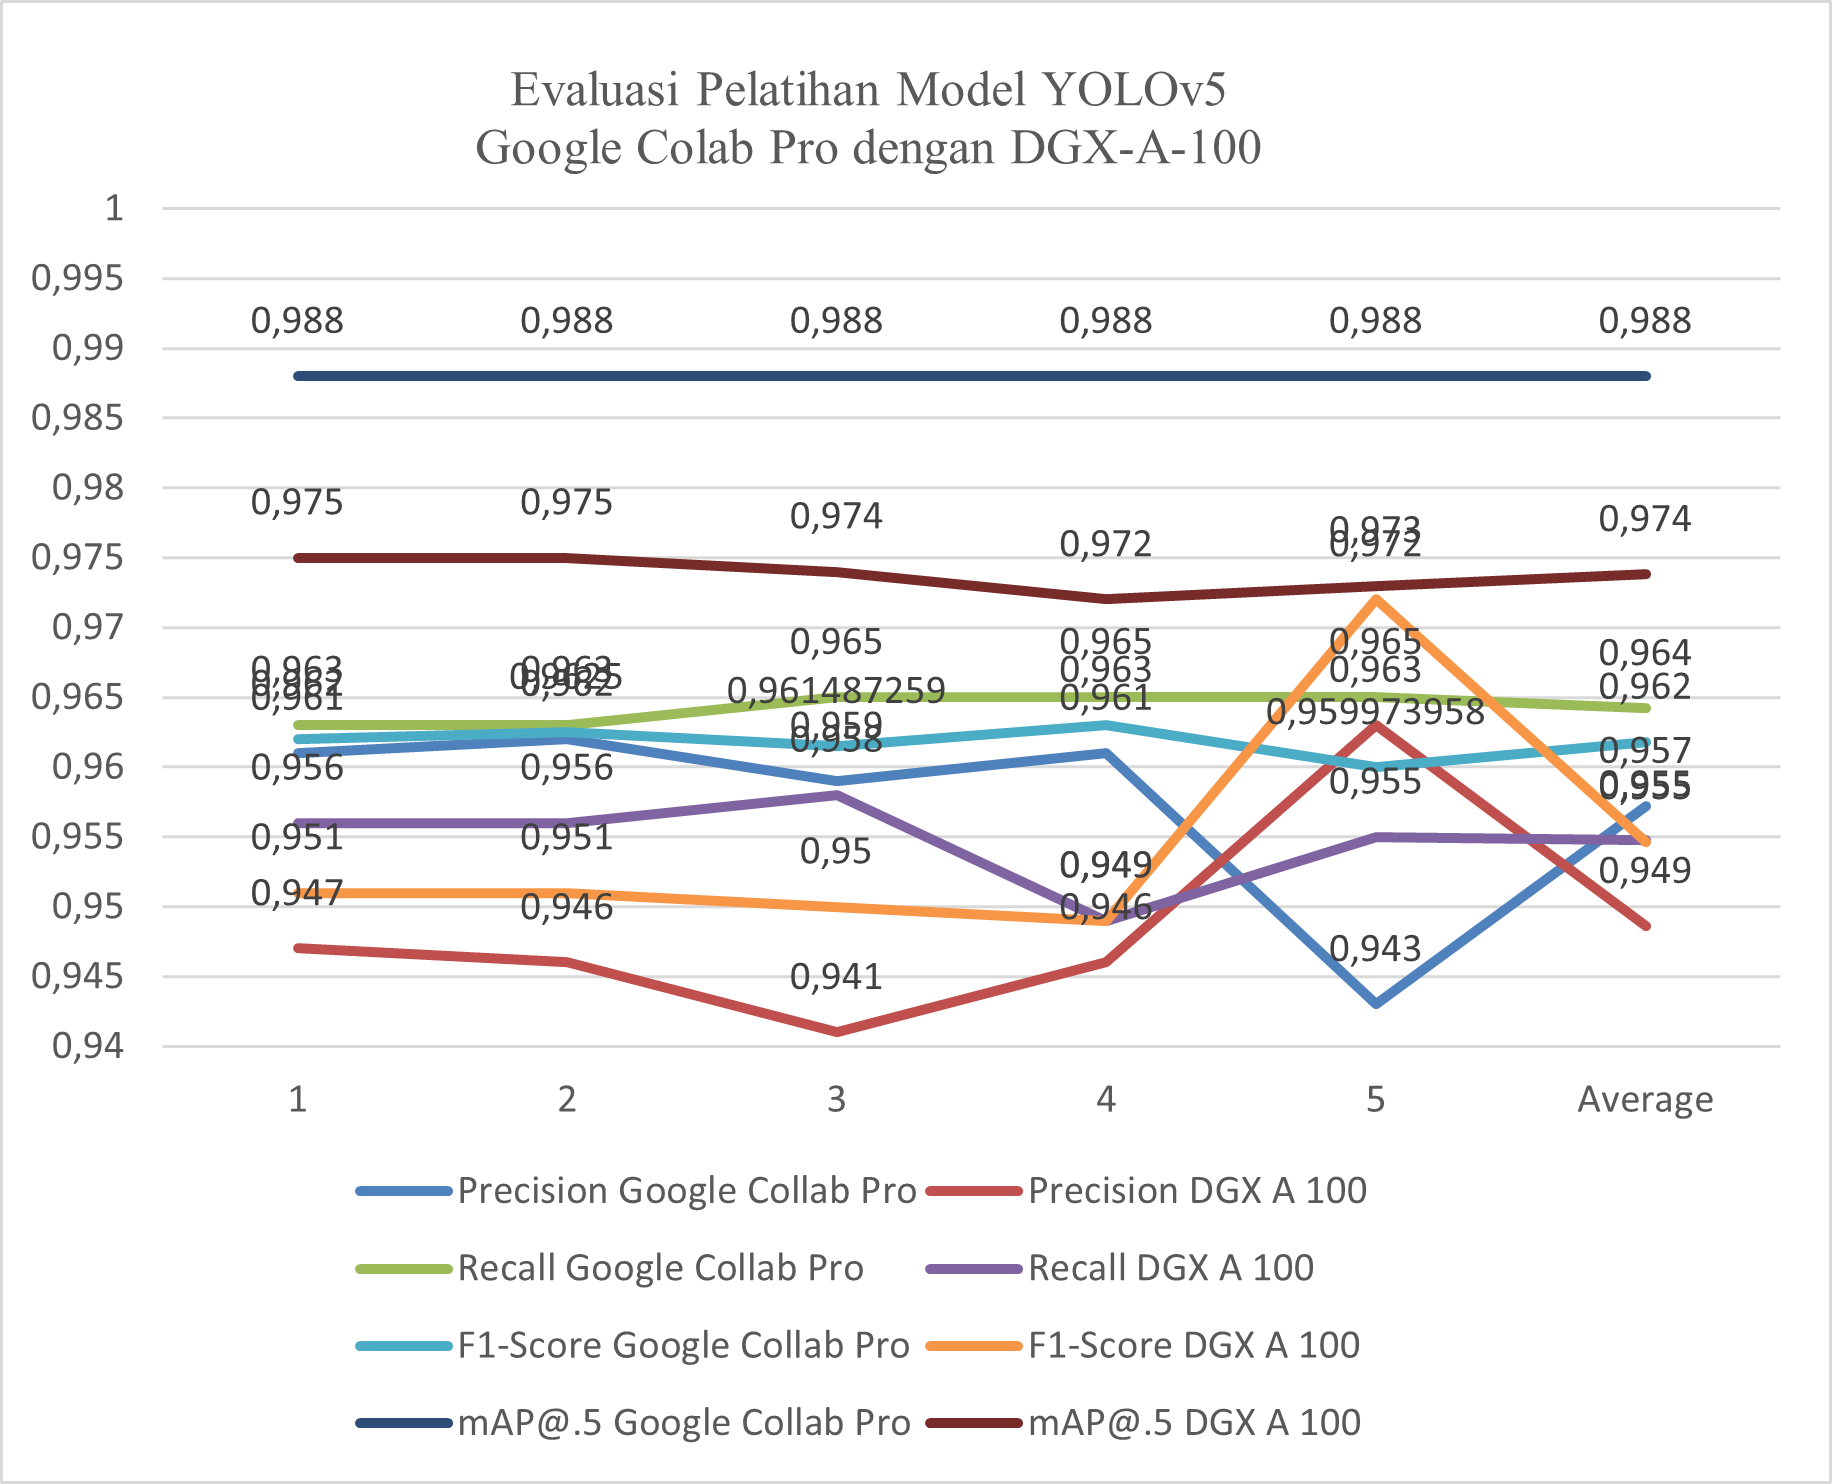
\includegraphics[width=1\columnwidth]{bab4/Gambar/Picture25.png}
	\end{center}
	\vspace{-0.2cm}
	%\rule{\columnwidth}{0.1pt}
	\captionsetup{justification=centering}
	\caption{Hasil Evaluasi Pelatihan Model YOLOv5 antara Google Colab Pro dengan DGX-A-100}\label{img:Hasil-Evaluasi-Pelatihan-Model-YOLOv5-Colab-DGX}
\end{figure}
%%%%%%%%%%%%%%%%%%%%%%%%%% GAMBAR %%%%%%%%%%%%%%%%%%%%%%%%%%%%%%

Hasil dari proses pelatihan ini juga membutuhkan waktu proses yang digunakan antara Google Colab Pro dengan DGX-A-100 milik Universitas Gunadarma yang tercantum pada Tabel \ref{tbl:Evaluasi-Waktu-Proses-Pelatihan-Model-CNN-YOLOv5}.

%%%%%%%%%%%%%%%%%%%%%%%TABEL SEDERHANA%%%%%%%%%%%%%%%%%%%%%%%%%
\begin{singlespace}
	\begin{table}[H]
		\centering
		\caption{Evaluasi Waktu Proses Pelatihan Model CNN YOLOv5}
		\label{tbl:Evaluasi-Waktu-Proses-Pelatihan-Model-CNN-YOLOv5}
		\begin{tabular}{|m{2cm}|m{5cm}m{5cm}|}
			\hline
			\rowcolor[HTML]{D9D9D9} 
			\cellcolor[HTML]{D9D9D9}                       & \multicolumn{2}{l|}{\cellcolor[HTML]{D9D9D9}Waktu yang Dibutuhkan Pelatihan} \\ \cline{2-3} 
			\rowcolor[HTML]{D9D9D9} 
			\multirow{-2}{*}{\cellcolor[HTML]{D9D9D9}Fold} & \multicolumn{1}{l|}{\cellcolor[HTML]{D9D9D9}Google Colab Pro}   & DGX A 100  \\ \hline
			1                                              & \multicolumn{1}{l|}{4727}                                       & 922        \\ \hline
			2                                              & \multicolumn{1}{l|}{4724}                                       & 918        \\ \hline
			3                                              & \multicolumn{1}{l|}{4695}                                       & 926        \\ \hline
			4                                              & \multicolumn{1}{l|}{4655}                                       & 900        \\ \hline
			5                                              & \multicolumn{1}{l|}{4708}                                       & 936        \\ \hline
			Rata-Rata                                      & \multicolumn{1}{l|}{4702}                                       & 920        \\ \hline
		\end{tabular}
	\end{table}
\end{singlespace}
%%%%%%%%%%%%%%%%%%%%%%%TABEL SEDERHANA%%%%%%%%%%%%%%%%%%%%%%%%%

Waktu proses yang dibutuhkan oleh Google Colab Pro rata-rata membutuhkan waktu 4702 detik untuk setiap fold yang harus dijalankan dengan 30 epoch dan 1 iterasi dengan 16 batch size, sedangkan waktu pada DGX-A-100 dibutuhkan 920 waktu DGX-A-100 dengan batch size 10. Perbedaan waktu ini, lebih baik waktu yang diproses pada DGX-A-100 milik Universitas Gunadarma. Berdasarkan data pada Tabel \ref{tbl:Evaluasi-Waktu-Proses-Pelatihan-Model-CNN-YOLOv5}, model k-fold terbaik pada fold ke 2 untuk pelatihan YOLOv5.

\subsection{Pelatihan Model CNN YOLOv6}
\hspace{1,2cm}
Pelatihan model kedua yaitu dengan model CNN YOLOv6 dengan menggunakan Google Colab Pro dan DGX-A-100. Batch size yang digunakan dalam satu iterasi sama-sama menggunakan 16 dan 30 epoch. Hasil evaluasi pelatihan model CNN dengan YOLOv6 tampak pada Tabel \ref{tbl:Evaluasi-Pelatihan-Model-Dengan-YOLOv6}

%%%%%%%%%%%%%%%%%%%%%%%TABEL SEDERHANA%%%%%%%%%%%%%%%%%%%%%%%%%
\begin{singlespace}
	\begin{table}[H]
		\centering
		\caption{Evaluasi Pelatihan Model dengan YOLOv6 pada Google Colab Pro dan DGX-A-100}
		\label{tbl:Evaluasi-Pelatihan-Model-Dengan-YOLOv6}
		\begin{tabular}{|p{1cm}|p{1cm}p{1cm}|p{1cm}p{1cm}|p{1cm}p{1cm}|p{1cm}p{1cm}|}
			\hline
			\rowcolor[HTML]{D9D9D9} 
			\cellcolor[HTML]{D9D9D9}                       & \multicolumn{2}{p{1cm}|}{\cellcolor[HTML]{D9D9D9}Precision}                    & \multicolumn{2}{p{1cm}|}{\cellcolor[HTML]{D9D9D9}Recall}                       & \multicolumn{2}{p{1cm}|}{\cellcolor[HTML]{D9D9D9}F1-Score}                     & \multicolumn{2}{p{1cm}|}{\cellcolor[HTML]{BFBFBF}{\color[HTML]{333333} mAP@.5}} \\ \cline{2-9} 
			\rowcolor[HTML]{D9D9D9} 
			\multirow{-2}{*}{\cellcolor[HTML]{D9D9D9}Fold} & \multicolumn{1}{p{1cm}|}{\cellcolor[HTML]{D9D9D9}Google Colab Pro} & DGX A 100 & \multicolumn{1}{p{1cm}|}{\cellcolor[HTML]{D9D9D9}Google Colab Pro} & DGX A 100 & \multicolumn{1}{p{1cm}|}{\cellcolor[HTML]{D9D9D9}Google Colab Pro} & DGX A 100 & \multicolumn{1}{p{1cm}|}{\cellcolor[HTML]{D9D9D9}Google Colab Pro}  & DGX A 100 \\ \hline
			
			1                                              & \multicolumn{1}{p{1cm}|}{0,944}                                    & 0,919     & \multicolumn{1}{p{1cm}|}{0,774}                                    & 0,738     & \multicolumn{1}{p{1cm}|}{0,85}                                     & 0,818     & \multicolumn{1}{p{1cm}|}{0,944}                                     & 0,918     \\ \hline
			
			2                                              & \multicolumn{1}{p{1cm}|}{0,945}                                    & 0,920     & \multicolumn{1}{p{1cm}|}{0,772}                                    & 0,736     & \multicolumn{1}{p{1cm}|}{0,85}                                     & 0,817     & \multicolumn{1}{p{1cm}|}{0,944}                                     & 0,919     \\ \hline
			
			3                                              & \multicolumn{1}{p{1cm}|}{0,943}                                    & 0,918     & \multicolumn{1}{p{1cm}|}{0,775}                                    & 0,742     & \multicolumn{1}{p{1cm}|}{0,85}                                     & 0,821     & \multicolumn{1}{p{1cm}|}{0,943}                                     & 0,918     \\ \hline
			
			4                                              & \multicolumn{1}{p{1cm}|}{0,944}                                    & 0,911     & \multicolumn{1}{p{1cm}|}{0,771}                                    & 0,736     & \multicolumn{1}{p{1cm}|}{0,848}                                    & 0,814     & \multicolumn{1}{p{1cm}|}{0,943}                                     & 0,918     \\ \hline
			
			5                                              & \multicolumn{1}{p{1cm}|}{0,944}                                    & 0,918     & \multicolumn{1}{p{1cm}|}{0,771}                                    & 0,739     & \multicolumn{1}{p{1cm}|}{0,848}                                    & 0,818     & \multicolumn{1}{p{1cm}|}{0,943}                                     & 0,917     \\ \hline
			
			Rata-Rata                                      & \multicolumn{1}{p{1cm}|}{0,944}                                    & 0,917     & \multicolumn{1}{p{1cm}|}{0,773}                                    & 0,738     & \multicolumn{1}{p{1cm}|}{0,849}                                    & 0,818     & \multicolumn{1}{p{1cm}|}{0,943}                                     & 0,918     \\ \hline
		\end{tabular}
	\end{table}
\end{singlespace}
%%%%%%%%%%%%%%%%%%%%%%%TABEL SEDERHANA%%%%%%%%%%%%%%%%%%%%%%%%%

Hasil pada Tabel tbl:Evaluasi-Pelatihan-Model-Dengan-YOLOv6 menunjukkan bahwa hasil evaluasi model dengan menggunakan mesin Google Colab Pro masih lebih tinggi dibandingkan dengan DGX-A-100, yaitu beruturut-turut sebesar 0,944, 0,773, 0,849, dan 0,943 dengan 4 evaluasi model. Nilai rata-rata Precision cukup tinggi berada di atas 0,90, tetapi recall di bawah 0,80, hal ini menunjukkan bahwa pada YOLOv6 rasio prediksi benar positif dibandingkan dengan keseluruhan data yang benar positif yaitu pohon kelapa sawit masih dibawah nilai dari proses pelatihan YOLOv5. Berikut ini hasil evaluasi performance dalam bentuk diagram tampak seperti pada Gambar \ref{img:Hasil-Evaluasi-Pelatihan-Model-YOLOv6-Colab-DGX}.

%%%%%%%%%%%%%%%%%%%%%%%%%% GAMBAR %%%%%%%%%%%%%%%%%%%%%%%%%%%%%%
\begin{figure}[H]
	\vspace{-0.1cm}
	%\rule{\columnwidth}{0.1pt}
	\begin{center}
		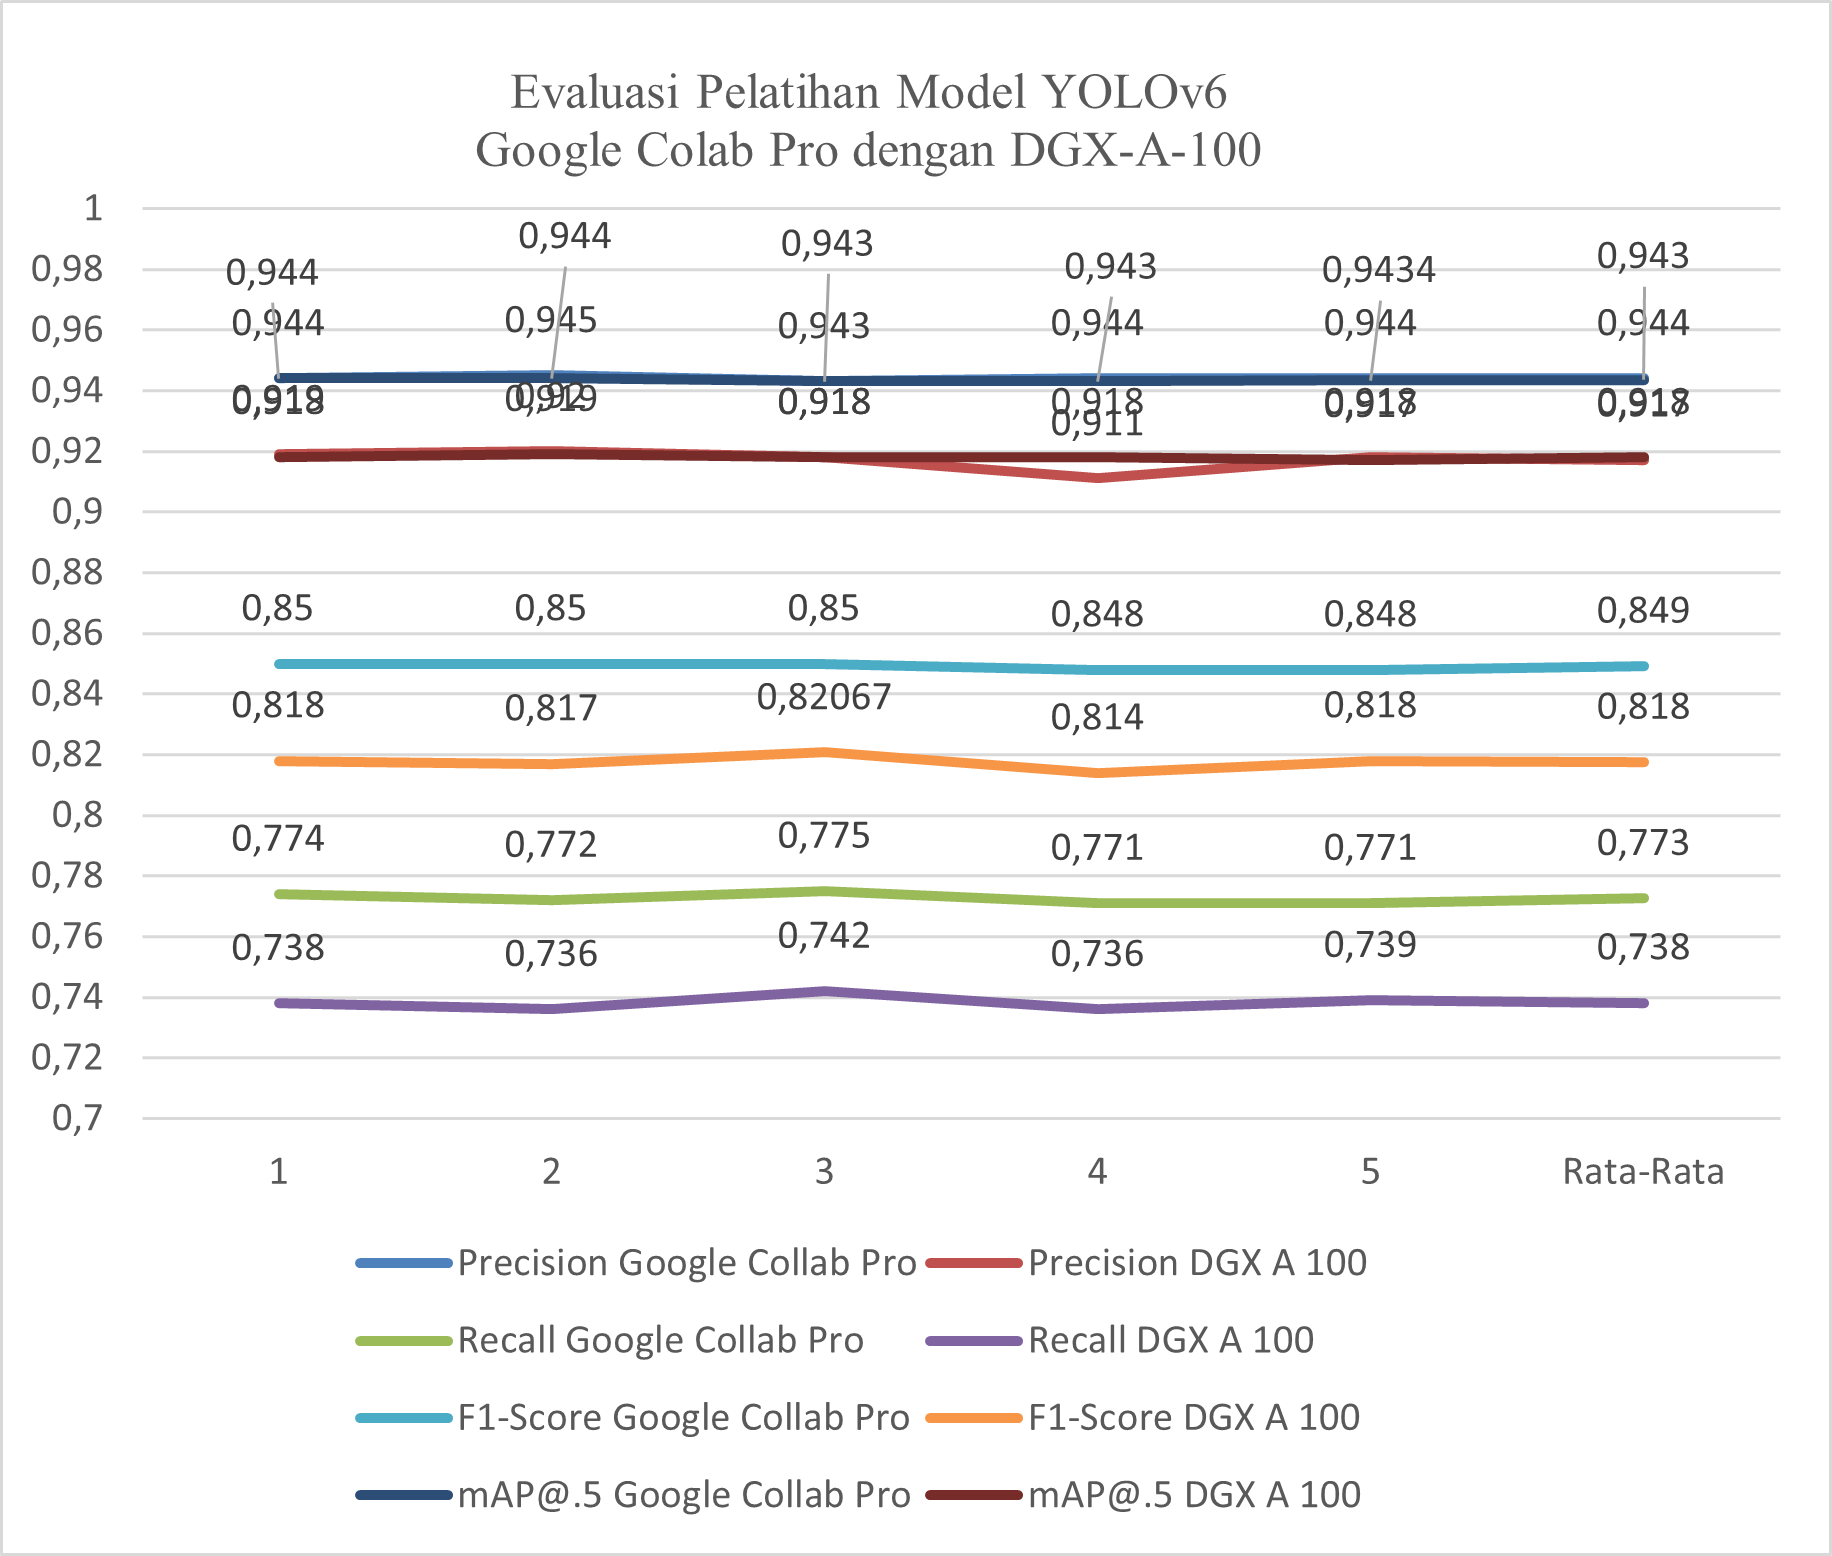
\includegraphics[width=1\columnwidth]{bab4/Gambar/Picture26.png}
	\end{center}
	\vspace{-0.2cm}
	%\rule{\columnwidth}{0.1pt}
	\captionsetup{justification=centering}
	\caption{Hasil Evaluasi Pelatihan Model YOLOv6 antara Google Colab Pro dengan DGX-A-100}\label{img:Hasil-Evaluasi-Pelatihan-Model-YOLOv6-Colab-DGX}
\end{figure}
%%%%%%%%%%%%%%%%%%%%%%%%%% GAMBAR %%%%%%%%%%%%%%%%%%%%%%%%%%%%%%

Sementara itu, Proses pelatihan ini juga membutuhkan waktu untuk pemrosesan pelatihan yang tampak pada Tabel \ref{tbl:Evaluasi-Waktu-Proses-Pelatihan-Model-CNN-YOLOv6}.

%%%%%%%%%%%%%%%%%%%%%%%TABEL SEDERHANA%%%%%%%%%%%%%%%%%%%%%%%%%
\begin{singlespace}
	\begin{table}[H]
		\centering
		\caption{Evaluasi Waktu Proses Pelatihan Model CNN YOLOv6}
		\label{tbl:Evaluasi-Waktu-Proses-Pelatihan-Model-CNN-YOLOv6}
		\begin{tabular}{|m{2cm}|m{5cm}m{5cm}|}
			\hline
			\rowcolor[HTML]{D9D9D9} 
			\cellcolor[HTML]{D9D9D9}                       & \multicolumn{2}{l|}{\cellcolor[HTML]{D9D9D9}Waktu yang Dibutuhkan Pelatihan} \\ \cline{2-3} 
			\rowcolor[HTML]{D9D9D9} 
			\multirow{-2}{*}{\cellcolor[HTML]{D9D9D9}Fold} & \multicolumn{1}{l|}{\cellcolor[HTML]{D9D9D9}Google Colab Pro}   & DGX A 100  \\ \hline
			1 & \multicolumn{1}{l|}{7359} & 2668 \\ \hline
			2 & \multicolumn{1}{l|}{6696} & 2618 \\ \hline
			3 & \multicolumn{1}{l|}{6689} & 2675 \\ \hline
			4 & \multicolumn{1}{l|}{6707} & 2657 \\ \hline
			5 & \multicolumn{1}{l|}{8957} & 2654 \\ \hline
			Rata-Rata & \multicolumn{1}{l|}{7282} & 2654 \\ \hline
		\end{tabular}
	\end{table}
\end{singlespace}
%%%%%%%%%%%%%%%%%%%%%%%TABEL SEDERHANA%%%%%%%%%%%%%%%%%%%%%%%%%

Waktu proses yang dibutuhkan oleh Google Colab Pro rata-rata membutuhkan waktu 7282 detik untuk setiap fold yang harus dijalankan dengan 30 epoch dan 1 iterasi dengan 16 batch size, sedangkan waktu pada DGX-A-100 dibutuhkan 2654 waktu DGX-A-100. Perbedaan waktu ini, lebih baik waktu yang diproses pada DGX-A-100 milik Universitas Gunadarma. Berdasarkan data pada Tabel \ref{tbl:Evaluasi-Waktu-Proses-Pelatihan-Model-CNN-YOLOv6}, model k-fold terbaik pada fold ke 2 untuk pelatihan YOLOv6.

\subsection{Pelatihan Model CNN YOLOv7}
\hspace{1,2cm}
Pelatihan model ketiga yaitu dengan model CNN YOLOv7 dengan menggunakan Google Colab Pro dan DGX-A-100. Batch size yang digunakan dalam pelatihan model ini dalam satu iterasi sama-sama menggunakan 16 batch size dan 30 epoch. Hasil evaluasi pelatihan model CNN dengan YOLOv7 tampak pada Tabel 4.18.

%%%%%%%%%%%%%%%%%%%%%%%TABEL SEDERHANA%%%%%%%%%%%%%%%%%%%%%%%%%
\begin{singlespace}
	\begin{table}[H]
		\centering
		\caption{Evaluasi Pelatihan Model dengan YOLOv7 pada Google Colab Pro dan DGX-A-100}
		\label{tbl:Evaluasi-Pelatihan-Model-Dengan-YOLOv7}
		\begin{tabular}{|p{1cm}|p{1cm}p{1cm}|p{1cm}p{1cm}|p{1cm}p{1cm}|p{1cm}p{1cm}|}
			\hline
			\rowcolor[HTML]{D9D9D9} 
			\cellcolor[HTML]{D9D9D9}                       & \multicolumn{2}{p{1cm}|}{\cellcolor[HTML]{D9D9D9}Precision}                    & \multicolumn{2}{p{1cm}|}{\cellcolor[HTML]{D9D9D9}Recall}                       & \multicolumn{2}{p{1cm}|}{\cellcolor[HTML]{D9D9D9}F1-Score}                     & \multicolumn{2}{p{1cm}|}{\cellcolor[HTML]{BFBFBF}{\color[HTML]{333333} mAP@.5}} \\ \cline{2-9} 
			\rowcolor[HTML]{D9D9D9} 
			\multirow{-2}{*}{\cellcolor[HTML]{D9D9D9}Fold} & \multicolumn{1}{p{1cm}|}{\cellcolor[HTML]{D9D9D9}Google Colab Pro} & DGX A 100 & \multicolumn{1}{p{1cm}|}{\cellcolor[HTML]{D9D9D9}Google Colab Pro} & DGX A 100 & \multicolumn{1}{p{1cm}|}{\cellcolor[HTML]{D9D9D9}Google Colab Pro} & DGX A 100 & \multicolumn{1}{p{1cm}|}{\cellcolor[HTML]{D9D9D9}Google Colab Pro}  & DGX A 100 \\ \hline
			
			1                                              & \multicolumn{1}{p{1cm}|}{0,967}                                    & 0,961     & \multicolumn{1}{p{1cm}|}{0,977}                                    & 0,970     & \multicolumn{1}{p{1cm}|}{0,972}                                    & 0,965     & \multicolumn{1}{p{1cm}|}{0,993}                                     & 0,989     \\ \hline
			
			2                                              & \multicolumn{1}{p{1cm}|}{0,970}                                    & 0,965     & \multicolumn{1}{p{1cm}|}{0,976}                                    & 0,966     & \multicolumn{1}{p{1cm}|}{0,973}                                    & 0,965     & \multicolumn{1}{p{1cm}|}{0,993}                                     & 0,989     \\ \hline
			
			3                                              & \multicolumn{1}{p{1cm}|}{0,967}                                    & 0,961     & \multicolumn{1}{p{1cm}|}{0,979}                                    & 0,970     & \multicolumn{1}{p{1cm}|}{0,973}                                    & 0,965     & \multicolumn{1}{p{1cm}|}{0,993}                                     & 0,989     \\ \hline
			
			4                                              & \multicolumn{1}{p{1cm}|}{0,972}                                    & 0,965     & \multicolumn{1}{p{1cm}|}{0,973}                                    & 0,966     & \multicolumn{1}{p{1cm}|}{0,973}                                    & 0,965     & \multicolumn{1}{p{1cm}|}{0,993}                                     & 0,989     \\ \hline
			
			5                                              & \multicolumn{1}{p{1cm}|}{0,971}                                    & 0,963     & \multicolumn{1}{p{1cm}|}{0,974}                                    & 0,964     & \multicolumn{1}{p{1cm}|}{0,972}                                    & 0,963     & \multicolumn{1}{p{1cm}|}{0,993}                                     & 0,988     \\ \hline
			
			Rata-Rata                                      & \multicolumn{1}{p{1cm}|}{0,969}                                    & 0,963     & \multicolumn{1}{p{1cm}|}{0,976}                                    & 0,967     & \multicolumn{1}{p{1cm}|}{0,973}                                    & 0,965     & \multicolumn{1}{p{1cm}|}{0,993}                                     & 0,989     \\ \hline
			
		\end{tabular}
	\end{table}
\end{singlespace}
%%%%%%%%%%%%%%%%%%%%%%%TABEL SEDERHANA%%%%%%%%%%%%%%%%%%%%%%%%%

Hasil pada Tabel \ref{tbl:Evaluasi-Pelatihan-Model-Dengan-YOLOv7} menunjukkan bahwa hasil evaluasi model dengan menggunakan mesin Google Colab Pro masih lebih tinggi dibandingkan dengan DGX-A-100, yaitu beruturut-turut sebesar 0,969, 0,976, 0,973, dan 0,993 dari 4 evaluasi model yang digunakan. Nilai rata-rata best mAP@.5 berada pada posisi nilai 0,993 yang dimana dari fold 1 hingga fold 5 berada pada nilai yang konsisten 0,993, hal ini membuktikan bahwa algoritma YOLOv7 mencapai akurasi tertinggi diantara model pendeteksian objek secara real-time lainnya, dan telah ditetapkan berdasarkan artikel secara resmi yang ditulis mengenai YOLOv7. Berikut ini hasil evaluasi performance dalam bentuk diagram tampak seperti pada Gambar \ref{img:Hasil-Evaluasi-Pelatihan-Model-YOLOv7-Colab-DGX}.

%%%%%%%%%%%%%%%%%%%%%%%%%% GAMBAR %%%%%%%%%%%%%%%%%%%%%%%%%%%%%%
\begin{figure}[H]
	\vspace{-0.1cm}
	%\rule{\columnwidth}{0.1pt}
	\begin{center}
		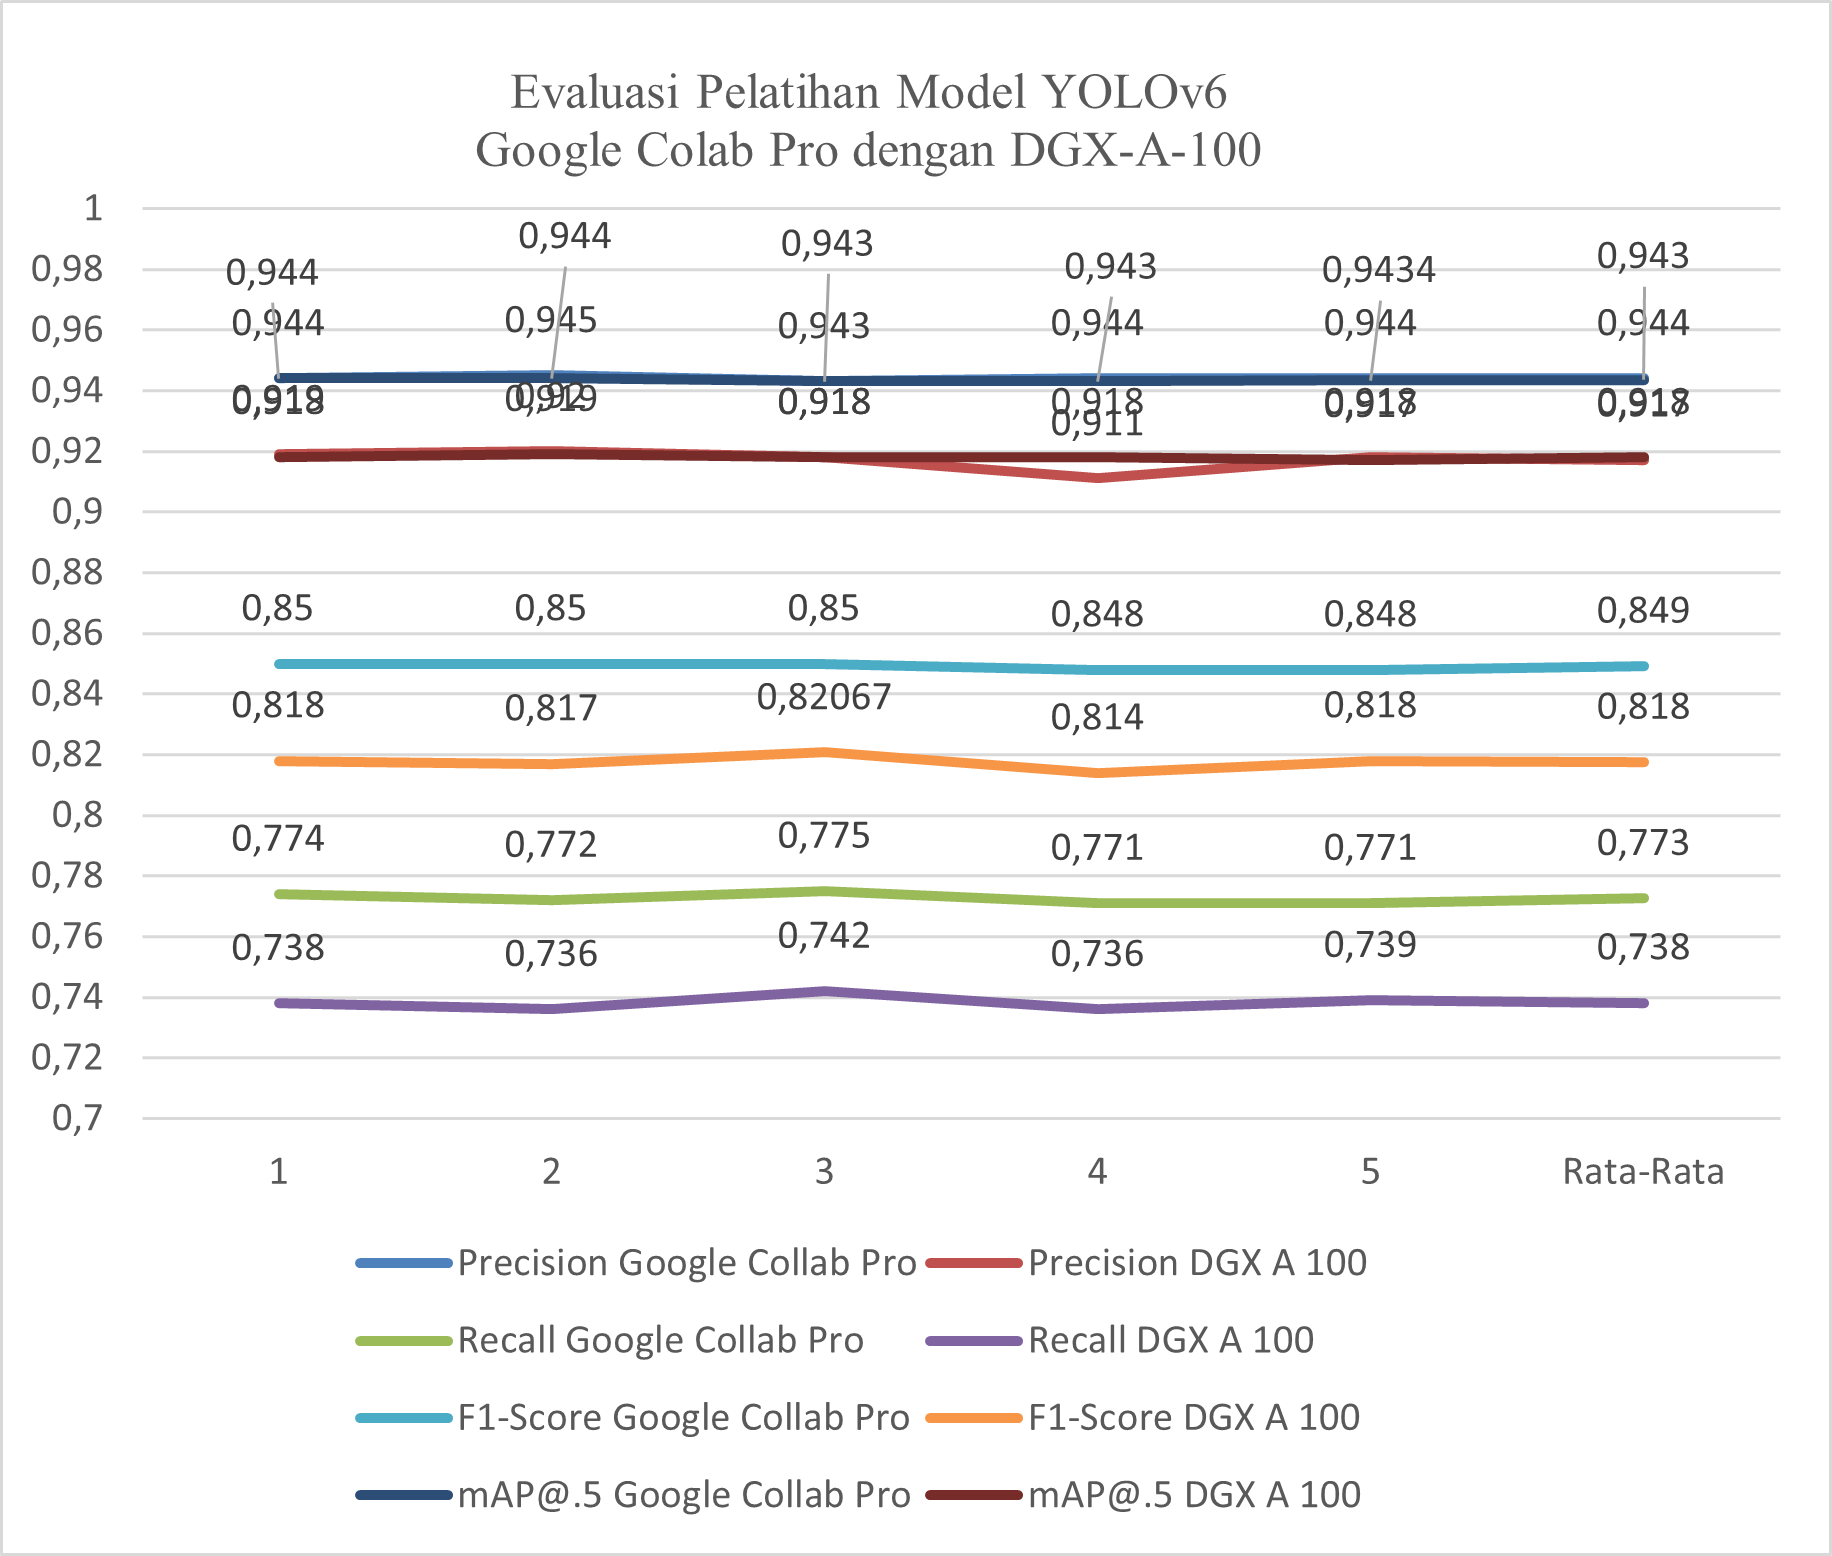
\includegraphics[width=1\columnwidth]{bab4/Gambar/Picture26.png}
	\end{center}
	\vspace{-0.2cm}
	%\rule{\columnwidth}{0.1pt}
	\captionsetup{justification=centering}
	\caption{Hasil Evaluasi Pelatihan Model YOLOv7 antara Google Colab Pro dengan DGX-A-100}\label{img:Hasil-Evaluasi-Pelatihan-Model-YOLOv7-Colab-DGX}
\end{figure}
%%%%%%%%%%%%%%%%%%%%%%%%%% GAMBAR %%%%%%%%%%%%%%%%%%%%%%%%%%%%%%

Selanjutnya, waktu proses pelatihan model pada YOLOv7 tampak pada Tabel 4.19.

%%%%%%%%%%%%%%%%%%%%%%%TABEL SEDERHANA%%%%%%%%%%%%%%%%%%%%%%%%%
\begin{singlespace}
	\begin{table}[H]
		\centering
		\caption{Evaluasi Waktu Proses Pelatihan Model CNN YOLOv7}
		\label{tbl:Evaluasi-Waktu-Proses-Pelatihan-Model-CNN-YOLOv7}
		\begin{tabular}{|m{2cm}|m{5cm}m{5cm}|}
			\hline
			\rowcolor[HTML]{D9D9D9} 
			\cellcolor[HTML]{D9D9D9}                       & \multicolumn{2}{l|}{\cellcolor[HTML]{D9D9D9}Waktu yang Dibutuhkan Pelatihan} \\ \cline{2-3} 
			\rowcolor[HTML]{D9D9D9} 
			\multirow{-2}{*}{\cellcolor[HTML]{D9D9D9}Fold} & \multicolumn{1}{l|}{\cellcolor[HTML]{D9D9D9}Google Colab Pro}   & DGX A 100  \\ \hline
			1                                              & \multicolumn{1}{l|}{4857}                                       & 2988        \\ \hline
			2                                              & \multicolumn{1}{l|}{4794}                                       & 2866        \\ \hline
			3                                              & \multicolumn{1}{l|}{4820}                                       & 2966        \\ \hline
			4                                              & \multicolumn{1}{l|}{4888}                                       & 2952        \\ \hline
			5                                              & \multicolumn{1}{l|}{4874}                                       & 2968        \\ \hline
			Rata-Rata                                      & \multicolumn{1}{l|}{4847}                                       & 2948        \\ \hline
		\end{tabular}
	\end{table}
\end{singlespace}
%%%%%%%%%%%%%%%%%%%%%%%TABEL SEDERHANA%%%%%%%%%%%%%%%%%%%%%%%%%

Waktu proses yang dibutuhkan untuk setiap fold yang harus dijalankan dengan 30 epoch dan 1 iterasi dengan 16 batch size oleh Google Colab Pro rata-rata membutuhkan waktu 4847 detik, sedangkan waktu pada DGX-A-100 dibutuhkan 2948 waktu. Perbedaan waktu ini, lebih baik waktu yang diproses pada DGX-A-100 milik Universitas Gunadarma. Berdasarkan data pada Tabel 4.19, model k-fold terbaik pada fold ke 2 untuk pelatihan YOLOv7. 

\section{Pengujian Model CNN}
\hspace{1,2cm}
Proses pelatihan dengan dataset pelatihan telah dilakukan, selanjutnya dilakukan proses pengujian dengan dataset uji. Dataset uji yang digunakan pada setiap k-fold yaitu 125 citra. Pada tahap ini dilakukan pengujian yang dilakukan pada model CNN YOLOv5, YOLOv6, dan YOLOv7. Pada proses pengujian ini juga menggunakan mesin super komputer DGX-A-100 milik Universitas Gunadarma dan Google Colab Pro.

\subsection{Pengujian Model CNN YOLOv5}
\hspace{1,2cm}
Pengujian model CNN yang pertama dengan menggunakan YOLOv5 dengan data citra pengujian sebanyak 125 citra pada 5 k-fold cross-validation. Pada proses pengujian ini batch size yang digunakan adalah 32 batch size yang berarti 32 jumlah sampel data yang melewati jaringan untuk setiap 1 iterasi atau putaran. Hasil dari pengujian model YOLOv5 dengan menggunakan mesin Google Colab Pro dan DGX-A-100 tampak pada Tabel \ref{tbl:Evaluasi-Pengujian-Model-Dengan-YOLOv5-Colab-DGX}.


%%%%%%%%%%%%%%%%%%%%%%%TABEL SEDERHANA%%%%%%%%%%%%%%%%%%%%%%%%%
\begin{singlespace}
	\begin{table}[H]
		\centering
		\caption{Evaluasi Pengujian Model dengan YOLOv5 pada Google Colab Pro dan DGX-A-100}
		\label{tbl:Evaluasi-Pengujian-Model-Dengan-YOLOv5-Colab-DGX}
		\begin{tabular}{|p{1cm}|p{1cm}p{1cm}|p{1cm}p{1cm}|p{1cm}p{1cm}|p{1cm}p{1cm}|}
			\hline
			\rowcolor[HTML]{D9D9D9} 
			\cellcolor[HTML]{D9D9D9}                       & \multicolumn{2}{p{1cm}|}{\cellcolor[HTML]{D9D9D9}Precision}                    & \multicolumn{2}{p{1cm}|}{\cellcolor[HTML]{D9D9D9}Recall}                       & \multicolumn{2}{p{1cm}|}{\cellcolor[HTML]{D9D9D9}F1-Score}                     & \multicolumn{2}{p{1cm}|}{\cellcolor[HTML]{BFBFBF}{\color[HTML]{333333} mAP@.5}} \\ \cline{2-9} 
			\rowcolor[HTML]{D9D9D9} 
			\multirow{-2}{*}{\cellcolor[HTML]{D9D9D9}Fold} & \multicolumn{1}{p{1cm}|}{\cellcolor[HTML]{D9D9D9}Google Colab Pro} & DGX A 100 & \multicolumn{1}{p{1cm}|}{\cellcolor[HTML]{D9D9D9}Google Colab Pro} & DGX A 100 & \multicolumn{1}{p{1cm}|}{\cellcolor[HTML]{D9D9D9}Google Colab Pro} & DGX A 100 & \multicolumn{1}{p{1cm}|}{\cellcolor[HTML]{D9D9D9}Google Colab Pro}  & DGX A 100 \\ \hline
			
			1                                              & \multicolumn{1}{p{1cm}|}{0,951}                                    & 0,805     & \multicolumn{1}{p{1cm}|}{0,970}                                    & 0,959     & \multicolumn{1}{p{1cm}|}{0,960}                                    & 0,875     & \multicolumn{1}{p{1cm}|}{0,989}                                     & 0,927     \\ \hline
			
			2                                              & \multicolumn{1}{p{1cm}|}{0,966}                                    & 0,800     & \multicolumn{1}{p{1cm}|}{0,976}                                    & 0,958     & \multicolumn{1}{p{1cm}|}{0,971}                                    & 0,872     & \multicolumn{1}{p{1cm}|}{0,992}                                     & 0,926     \\ \hline
			
			3                                              & \multicolumn{1}{p{1cm}|}{0,945}                                    & 0,799     & \multicolumn{1}{p{1cm}|}{0,969}                                    & 0,671     & \multicolumn{1}{p{1cm}|}{0,957}                                    & 0,729     & \multicolumn{1}{p{1cm}|}{0,987}                                     & 0,673     \\ \hline
			
			4                                              & \multicolumn{1}{p{1cm}|}{0,955}                                    & 0,809     & \multicolumn{1}{p{1cm}|}{0,969}                                    & 0,955     & \multicolumn{1}{p{1cm}|}{0,962}                                    & 0,876     & \multicolumn{1}{p{1cm}|}{0,988}                                     & 0,934     \\ \hline
			
			5                                              & \multicolumn{1}{p{1cm}|}{0,947}                                    & 0,811     & \multicolumn{1}{p{1cm}|}{0,969}                                    & 0,956     & \multicolumn{1}{p{1cm}|}{0,958}                                    & 0,878     & \multicolumn{1}{p{1cm}|}{0,987}                                     & 0,936     \\ \hline
			
			Rata-rata                                      & \multicolumn{1}{p{1cm}|}{0,953}                                    & 0,805     & \multicolumn{1}{p{1cm}|}{0,971}                                    & 0,900     & \multicolumn{1}{p{1cm}|}{0,962}                                    & 0,846     & \multicolumn{1}{p{1cm}|}{0,989}                                     & 0,879     \\ \hline
			
		\end{tabular}
	\end{table}
\end{singlespace}
%%%%%%%%%%%%%%%%%%%%%%%TABEL SEDERHANA%%%%%%%%%%%%%%%%%%%%%%%%%

Hasil pengujian menunjukkan bahwa hasil best \textit{mean average} (best mAP) untuk YOLOv5 dengan mesin Google Colab Pro lebih tinggi yaitu sebesar 0,989 dibandingkan dengan DGX-A-100 sebesar 0,879. Hasil ini menampilkan bahwa rata-rata presisi pada kelas pohon kelapa sawit di pengujian signifikan. Sebaran hasil pengujian model dengan YOLOv5 tampak seperti pada Gambar \ref{img:Hasil-Evaluasi-Pengujian-Model-YOLOv5-Colab-DGX}.


%%%%%%%%%%%%%%%%%%%%%%%%%% GAMBAR %%%%%%%%%%%%%%%%%%%%%%%%%%%%%%
\begin{figure}[H]
	\vspace{-0.1cm}
	%\rule{\columnwidth}{0.1pt}
	\begin{center}
		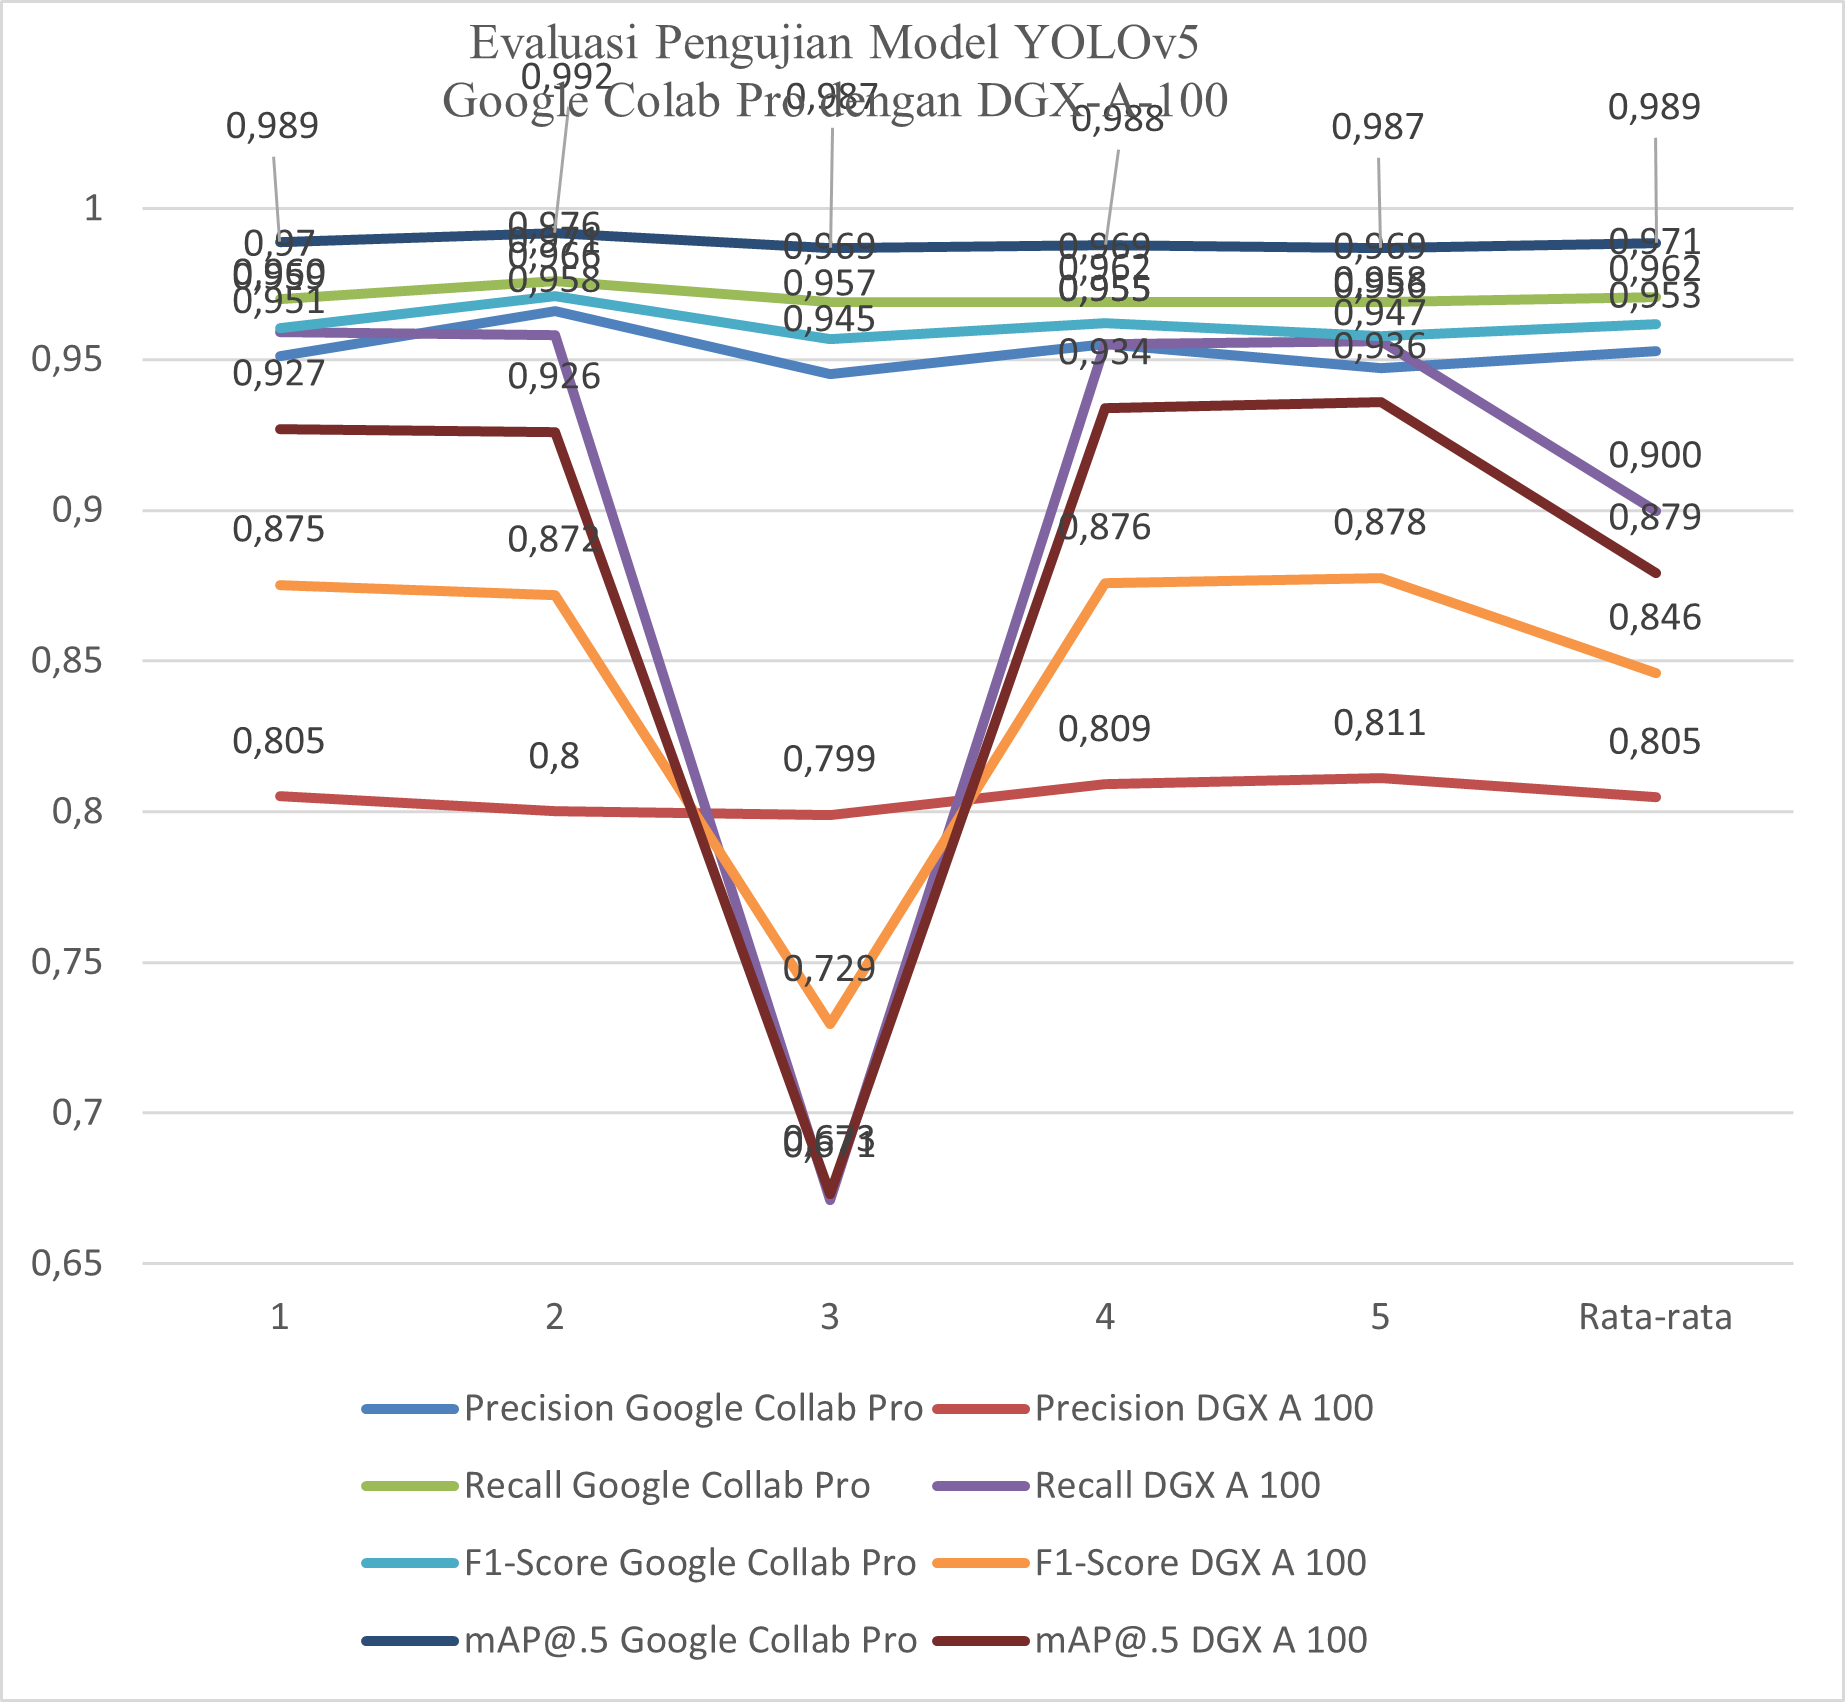
\includegraphics[width=1\columnwidth]{bab4/Gambar/Picture28.png}
	\end{center}
	\vspace{-0.2cm}
	%\rule{\columnwidth}{0.1pt}
	\captionsetup{justification=centering}
	\caption{Hasil Evaluasi Pengujian Model YOLOv5 antara Google Colab Pro dengan DGX-A-100}\label{img:Hasil-Evaluasi-Pengujian-Model-YOLOv5-Colab-DGX}
\end{figure}
%%%%%%%%%%%%%%%%%%%%%%%%%% GAMBAR %%%%%%%%%%%%%%%%%%%%%%%%%%%%%%

Dari hasil gambar menunjukkan bahwa best mAP terendah bernilai di bawah 0,70 pada mesin DGX-A-100 pada fold ke-3. Hal ini disebabkan bahwa pada fold 3 nilai rata-rata presisi cukup rendah untuk mendeteksi dengan benar bahwa itu adalah objek pohon kelapa sawit, kemudian hasil naik kembali pada fold ke 4 dan 5.

Waktu yang dibutuhkan untuk proses pengujian ini adalah tampak pada Tabel \ref{tbl:Evaluasi-Waktu-Proses-Pengujian-Model-CNN-YOLOv5}. 

%%%%%%%%%%%%%%%%%%%%%%%TABEL SEDERHANA%%%%%%%%%%%%%%%%%%%%%%%%%
\begin{singlespace}
	\begin{table}[H]
		\centering
		\caption{Evaluasi Waktu Proses Pengujian Model CNN YOLOv5}
		\label{tbl:Evaluasi-Waktu-Proses-Pengujian-Model-CNN-YOLOv5}
		\begin{tabular}{|l|ll|}
			\hline
			\rowcolor[HTML]{D9D9D9} 
			\cellcolor[HTML]{D9D9D9}                       & \multicolumn{2}{l|}{\cellcolor[HTML]{D9D9D9}Waktu (detik)}                \\ \cline{2-3} 
			\rowcolor[HTML]{D9D9D9} 
			\multirow{-2}{*}{\cellcolor[HTML]{D9D9D9}Fold} & \multicolumn{1}{l|}{\cellcolor[HTML]{D9D9D9}Google Colab Pro} & DGX A 100 \\ \hline
			1                                              & \multicolumn{1}{l|}{122}                                      & 54        \\ \hline
			2                                              & \multicolumn{1}{l|}{119}                                      & 50        \\ \hline
			3                                              & \multicolumn{1}{l|}{118}                                      & 54        \\ \hline
			4                                              & \multicolumn{1}{l|}{122}                                      & 52        \\ \hline
			5                                              & \multicolumn{1}{l|}{123}                                      & 54        \\ \hline
			Rata-Rata                                      & \multicolumn{1}{l|}{121}                                      & 53        \\ \hline
		\end{tabular}
	\end{table}
\end{singlespace}
%%%%%%%%%%%%%%%%%%%%%%%TABEL SEDERHANA%%%%%%%%%%%%%%%%%%%%%%%%%

Hasil dari waktu proses pengujian model dengan 125 data citra pada YOLOv5 oleh Google Colab Pro rata-rata membutuhkan waktu 121 detik, sedangkan waktu pada DGX-A-100 dibutuhkan 53 detik. Perbedaan waktu ini, lebih baik waktu yang diproses pada DGX-A-100 milik Universitas Gunadarma. Waktu komputasi pengujian lebih baik pada penggunan DGX-A-100. 

Berdasarkan hasil pengujian tersebut, berikut ini hasil confusion matrix dan hasil keluaran pada dataset pengujian pada Gambar \ref{img:Confusion-Matrix-dan-Citra-Sampel-Prediksi-Pohon-Kelapa} (a) dan (b).

%%%%%%%%%%%%%%%%%%%%%%%%%% GAMBAR %%%%%%%%%%%%%%%%%%%%%%%%%%%%%%
\begin{figure}[H]
	\vspace{-0.1cm}
	%\rule{\columnwidth}{0.1pt}
	\begin{center}
		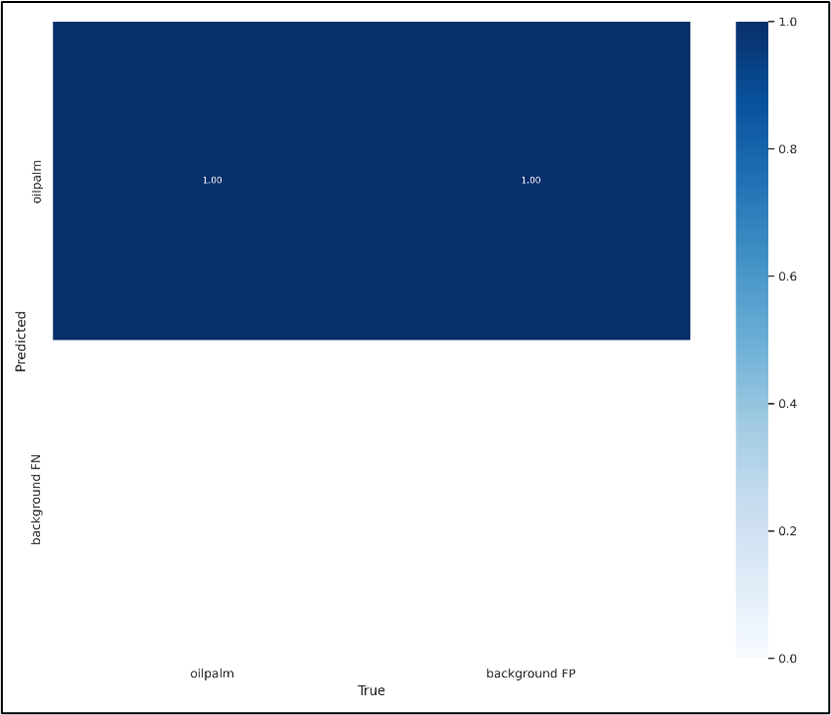
\includegraphics[width=1\columnwidth]{bab4/Gambar/Picture29.1.png}
		(a)
	\end{center}
	\vspace{-0.2cm}
	%\rule{\columnwidth}{0.1pt}
	%\captionsetup{justification=centering}
	%\caption{(a) Confusion Matrix dan (b) Citra Sampel Prediksi Pohon Kelapa Sawit dari Citra Dataset Pengujian}\label{img:Confusion-Matrix-dan-Citra-Sampel-Prediksi-Pohon-Kelapa}
\end{figure}
%%%%%%%%%%%%%%%%%%%%%%%%%% GAMBAR %%%%%%%%%%%%%%%%%%%%%%%%%%%%%%

%%%%%%%%%%%%%%%%%%%%%%%%%% GAMBAR %%%%%%%%%%%%%%%%%%%%%%%%%%%%%%
\begin{figure}[H]
	\vspace{-0.1cm}
	%\rule{\columnwidth}{0.1pt}
	\begin{center}
		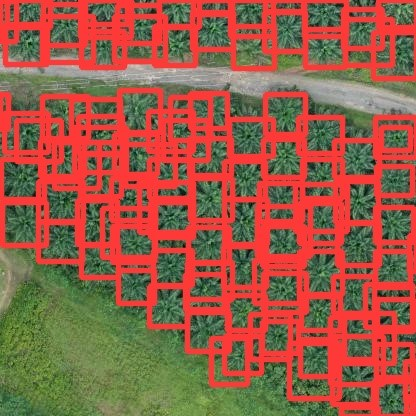
\includegraphics[width=1\columnwidth]{bab4/Gambar/Picture29.2.jpg}
		(b)
	\end{center}
	\vspace{-0.2cm}
	%\rule{\columnwidth}{0.1pt}
	\captionsetup{justification=centering}
	\caption{(a) Confusion Matrix dan (b) Citra Sampel Prediksi Pohon Kelapa Sawit dari Citra Dataset Pengujian}\label{img:Confusion-Matrix-dan-Citra-Sampel-Prediksi-Pohon-Kelapa}
\end{figure}
%%%%%%%%%%%%%%%%%%%%%%%%%% GAMBAR %%%%%%%%%%%%%%%%%%%%%%%%%%%%%%

Gambar \ref{img:Confusion-Matrix-dan-Citra-Sampel-Prediksi-Pohon-Kelapa}. menunjukkan confusion matrik yang bernilai positif, bahwa hasil menunjukkan nilai 1.00 pada oil palm, hal ini berarti model dapat berhasil memprediksi dengan benar bahwa objek tersebut merupakan oil palm (pohon kelapa sawit) dataset citra  pengujian, dan yang gambar yang sebelah kanan merupakan hasil pengujian dengan menampilkan kotak batas (\textit{bounding box}) yang disertai nilai \textit{confidence} yang menunjukkan bahwa nilai tersebut termasuk ke dalam kelas oil palm. Berdasarkan data pada Tabel \ref{tbl:Evaluasi-Waktu-Proses-Pengujian-Model-CNN-YOLOv5}, k-fold terbaik pada fold ke 2 untuk pengujian YOLOv5.

\subsection{Pengujian Model CNN YOLOv6}
\hspace{1,2cm}
Pengujian model yang kedua menggunakan model YOLOv6. Input image dengan menggunakan 640 x 640 dan batch size yang digunakan 32 batch size untuk satu iterasi. Hasil pengujian model dengan dua mesin yang digunakan, tampak seperti pada Tabel \ref{tbl:Evaluasi-Pengujian-Model-Dengan-YOLOv6-Colab-DGX}.

%%%%%%%%%%%%%%%%%%%%%%%TABEL SEDERHANA%%%%%%%%%%%%%%%%%%%%%%%%%
\begin{singlespace}
	\begin{table}[H]
		\centering
		\caption{Evaluasi Pengujian Model dengan YOLOv6 pada Google Colab Pro dan DGX-A-100}
		\label{tbl:Evaluasi-Pengujian-Model-Dengan-YOLOv6-Colab-DGX}
		\begin{tabular}{|p{1cm}|p{1cm}p{1cm}|p{1cm}p{1cm}|p{1cm}p{1cm}|p{1cm}p{1cm}|}
			\hline
			\rowcolor[HTML]{D9D9D9} 
			\cellcolor[HTML]{D9D9D9}                       & \multicolumn{2}{p{1cm}|}{\cellcolor[HTML]{D9D9D9}Precision}                    & \multicolumn{2}{p{1cm}|}{\cellcolor[HTML]{D9D9D9}Recall}                       & \multicolumn{2}{p{1cm}|}{\cellcolor[HTML]{D9D9D9}F1-Score}                     & \multicolumn{2}{p{1cm}|}{\cellcolor[HTML]{BFBFBF}{\color[HTML]{333333} mAP@.5}} \\ \cline{2-9} 
			\rowcolor[HTML]{D9D9D9} 
			\multirow{-2}{*}{\cellcolor[HTML]{D9D9D9}Fold} & \multicolumn{1}{p{1cm}|}{\cellcolor[HTML]{D9D9D9}Google Colab Pro} & DGX A 100 & \multicolumn{1}{p{1cm}|}{\cellcolor[HTML]{D9D9D9}Google Colab Pro} & DGX A 100 & \multicolumn{1}{p{1cm}|}{\cellcolor[HTML]{D9D9D9}Google Colab Pro} & DGX A 100 & \multicolumn{1}{p{1cm}|}{\cellcolor[HTML]{D9D9D9}Google Colab Pro}  & DGX A 100 \\ \hline
			
			1                                              & \multicolumn{1}{p{1cm}|}{0,801}                                    & 0,826     & \multicolumn{1}{p{1cm}|}{0,949}                                    & 0,880     & \multicolumn{1}{p{1cm}|}{0,869}                                    & 0,852     & \multicolumn{1}{p{1cm}|}{0,902}                                     & 0,866     \\ \hline
			
			2                                              & \multicolumn{1}{p{1cm}|}{0,819}                                    & 0,788     & \multicolumn{1}{p{1cm}|}{0,930}                                    & 0,920     & \multicolumn{1}{p{1cm}|}{0,871}                                    & 0,849     & \multicolumn{1}{p{1cm}|}{0,903}                                     & 0,870     \\ \hline
			
			3                                              & \multicolumn{1}{p{1cm}|}{0,805}                                    & 0,795     & \multicolumn{1}{p{1cm}|}{0,946}                                    & 0,910     & \multicolumn{1}{p{1cm}|}{0,870}                                    & 0,849     & \multicolumn{1}{p{1cm}|}{0,902}                                     & 0,872     \\ \hline
			
			4                                              & \multicolumn{1}{p{1cm}|}{0,815}                                    & 0,784     & \multicolumn{1}{p{1cm}|}{0,939}                                    & 0,920     & \multicolumn{1}{p{1cm}|}{0,873}                                    & 0,847     & \multicolumn{1}{p{1cm}|}{0,902}                                     & 0,871     \\ \hline
			
			5                                              & \multicolumn{1}{p{1cm}|}{0,804}                                    & 0,795     & \multicolumn{1}{p{1cm}|}{0,949}                                    & 0,910     & \multicolumn{1}{p{1cm}|}{0,871}                                    & 0,849     & \multicolumn{1}{p{1cm}|}{0,912}                                     & 0,872     \\ \hline
			
			Rata-rata                                      & \multicolumn{1}{p{1cm}|}{0,809}                                    & 0,798     & \multicolumn{1}{p{1cm}|}{0,943}                                    & 0,908     & \multicolumn{1}{p{1cm}|}{0,871}                                    & 0,849     & \multicolumn{1}{p{1cm}|}{0,898}                                     & 0,870     \\ \hline
			
		\end{tabular}
	\end{table}
\end{singlespace}
%%%%%%%%%%%%%%%%%%%%%%%TABEL SEDERHANA%%%%%%%%%%%%%%%%%%%%%%%%%

Berdasarkan Tabel \ref{tbl:Evaluasi-Pengujian-Model-Dengan-YOLOv6-Colab-DGX} hasil terbaik pada best mAP fold ke 5, dengan nilai rata-rata terbaik presisi sebesari 0,912 dan berdasarkan hasil rata-rata best mAP dengan Google Colab Pro juga lebih tinggi dibandingkan dengan DGX-A-100. Hasil sebaran evaluasi pengujian model dengan YOLOv6 seperti tampak pada Gambar \ref{img:Hasil-Evaluasi-Pengujian-Model-YOLOv6-Colab-DGX}. 

%%%%%%%%%%%%%%%%%%%%%%%%%% GAMBAR %%%%%%%%%%%%%%%%%%%%%%%%%%%%%%
\begin{figure}[H]
	\vspace{-0.1cm}
	%\rule{\columnwidth}{0.1pt}
	\begin{center}
		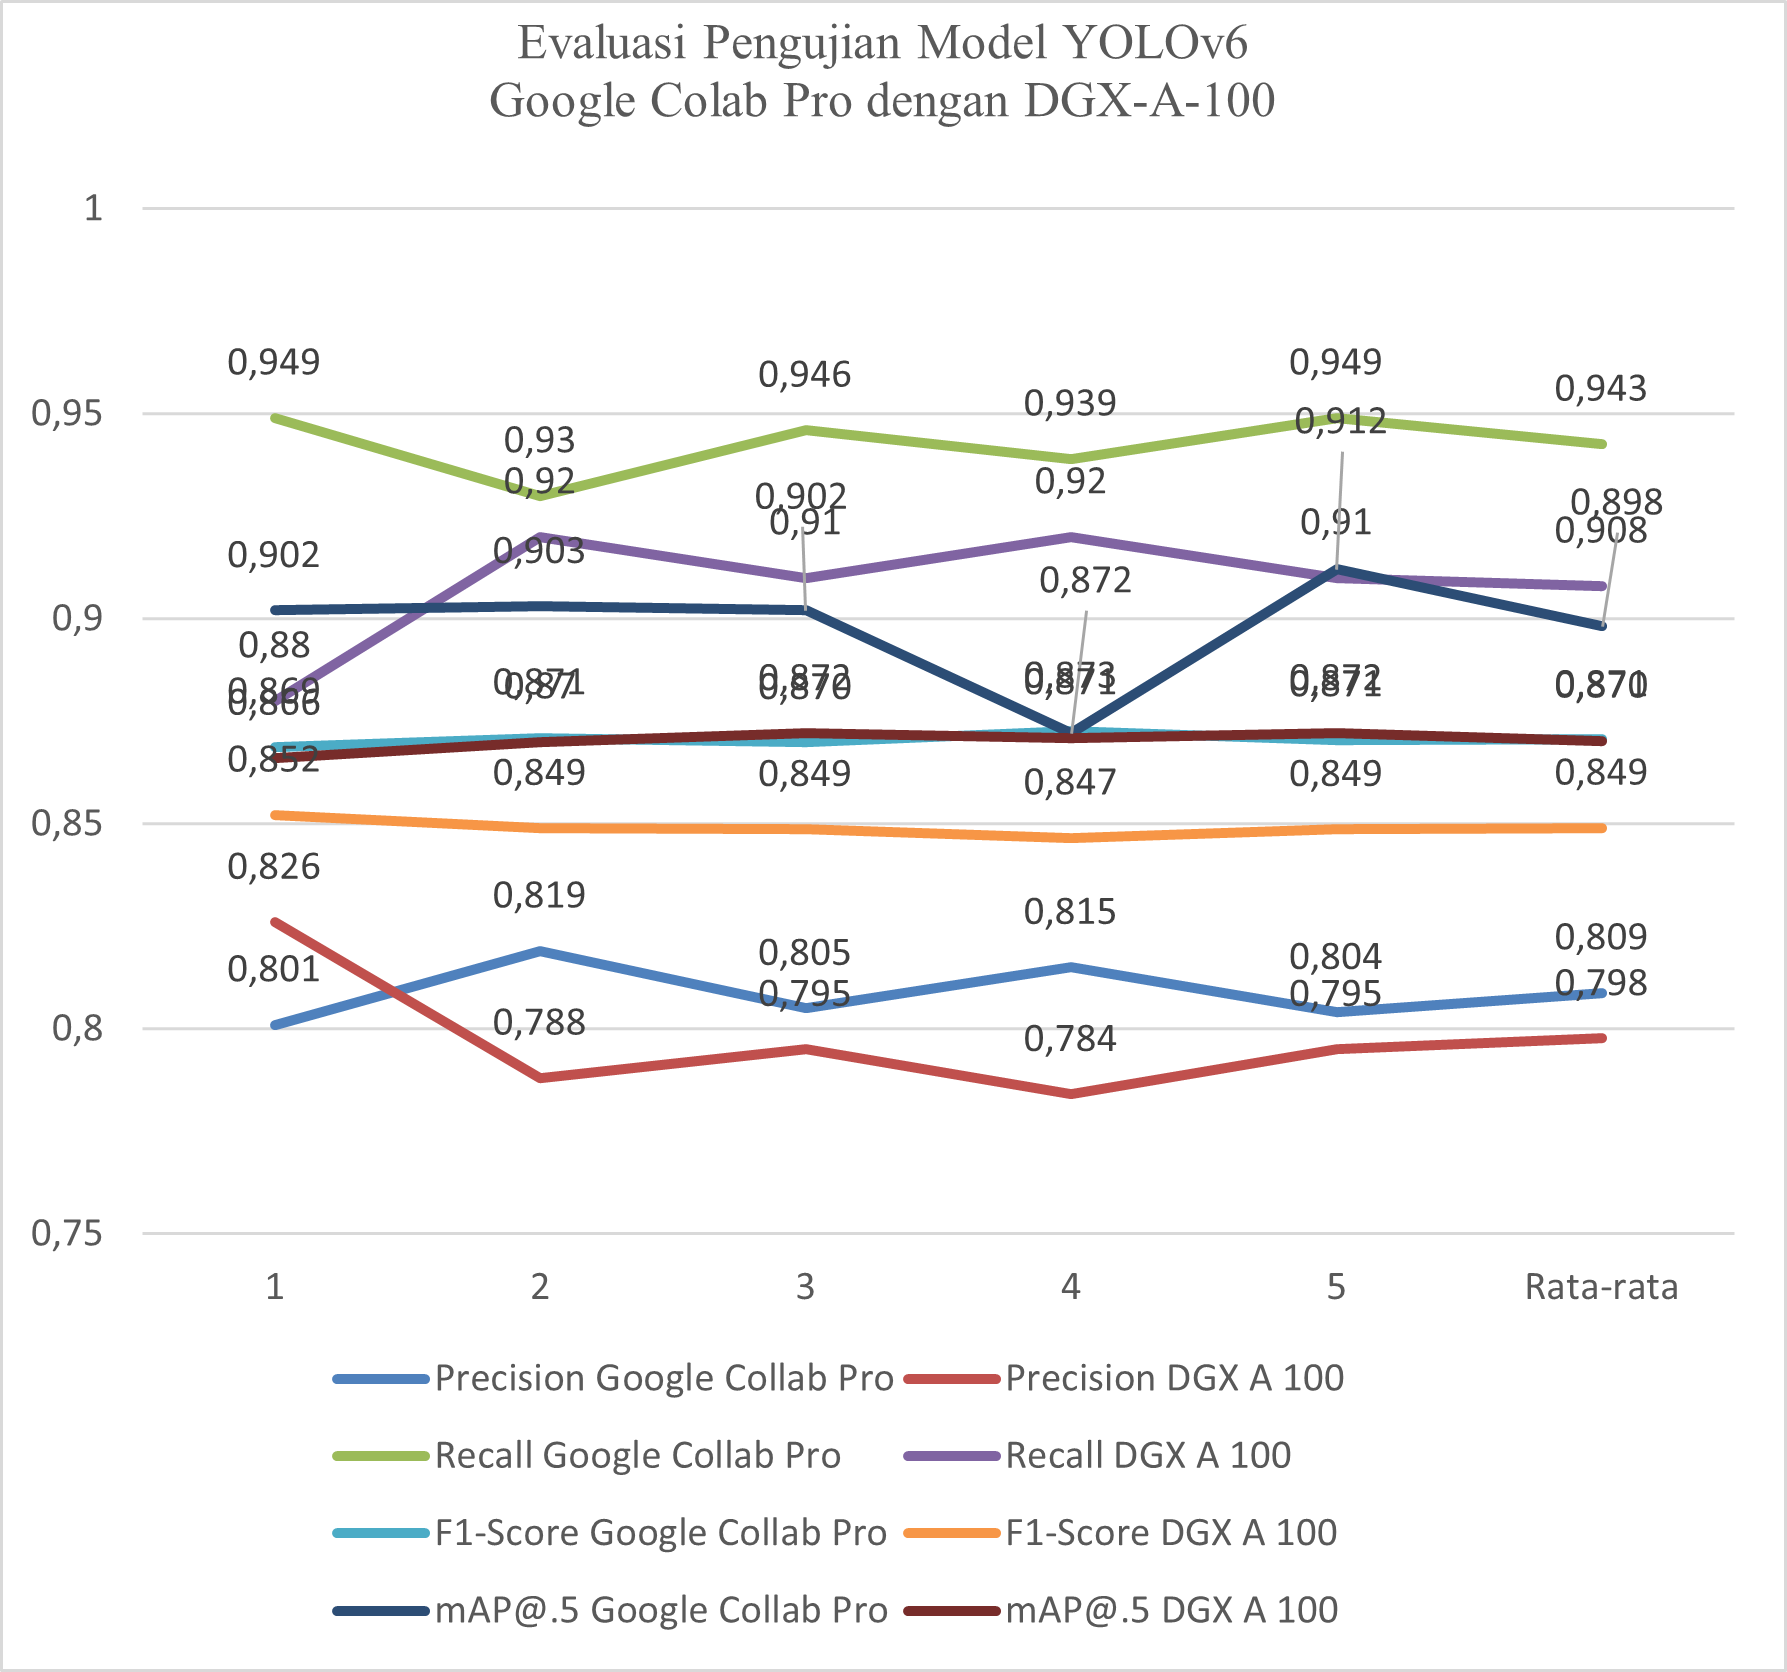
\includegraphics[width=1\columnwidth]{bab4/Gambar/Picture30.png}
	\end{center}
	\vspace{-0.2cm}
	%\rule{\columnwidth}{0.1pt}
	\captionsetup{justification=centering}
	\caption{Hasil Evaluasi Pengujian Model YOLOv6 antara Google Colab Pro dengan DGX-A-100}\label{img:Hasil-Evaluasi-Pengujian-Model-YOLOv6-Colab-DGX}
\end{figure}
%%%%%%%%%%%%%%%%%%%%%%%%%% GAMBAR %%%%%%%%%%%%%%%%%%%%%%%%%%%%%%

Berdasarkan dari waktu yang dibutuhkan pada proses pengujian model pada YOLOv6 dengan DGX-A-100 lebih cepat dibandingkan dengan Google Colab Pro. Hasil tampak pada Tabel \ref{tbl:Evaluasi-Waktu-Proses-Pengujian-Model-CNN-YOLOv6}.


%%%%%%%%%%%%%%%%%%%%%%%TABEL SEDERHANA%%%%%%%%%%%%%%%%%%%%%%%%%
\begin{singlespace}
	\begin{table}[H]
		\centering
		\caption{Evaluasi Waktu Proses Pengujian Model CNN YOLOv6}
		\label{tbl:Evaluasi-Waktu-Proses-Pengujian-Model-CNN-YOLOv6}
		\begin{tabular}{|l|ll|}
			\hline
			\rowcolor[HTML]{D9D9D9} 
			\cellcolor[HTML]{D9D9D9}                       & \multicolumn{2}{l|}{\cellcolor[HTML]{D9D9D9}Waktu (detik)}                \\ \cline{2-3} 
			\rowcolor[HTML]{D9D9D9} 
			\multirow{-2}{*}{\cellcolor[HTML]{D9D9D9}Fold} & \multicolumn{1}{l|}{\cellcolor[HTML]{D9D9D9}Google Colab Pro} & DGX A 100 \\ \hline
			1                                              & \multicolumn{1}{l|}{54}                                      & 53        \\ \hline
			2                                              & \multicolumn{1}{l|}{56}                                      & 53        \\ \hline
			3                                              & \multicolumn{1}{l|}{59}                                      & 50        \\ \hline
			4                                              & \multicolumn{1}{l|}{57}                                      & 52        \\ \hline
			5                                              & \multicolumn{1}{l|}{59}                                      & 50        \\ \hline
			Rata-Rata                                      & \multicolumn{1}{l|}{57}                                      & 54        \\ \hline
		\end{tabular}
	\end{table}
\end{singlespace}
%%%%%%%%%%%%%%%%%%%%%%%TABEL SEDERHANA%%%%%%%%%%%%%%%%%%%%%%%%%

Hasil dari waktu proses pengujian model pada YOLOv6 dengan data pengujian 125 citra, dihasilkan waktu yang tidak terlalu berbeda. Waktu yang dibutuhkan oleh Google Colab Pro rata-rata membutuhkan waktu 57 detik, sedangkan waktu pada DGX-A-100 dibutuhkan 54 detik. Perbedaan waktu ini, waktu DGX-A-100 lebih baik dibandingkan dengan DGX-A-100.

Berdasarkan hasil dari pengujian YOLOv6 pada Tabel \ref{tbl:Evaluasi-Waktu-Proses-Pengujian-Model-CNN-YOLOv6}, pada Gambar 4.31. merupakan \textit{confusion matriks} dari pengujian YOLOv6.


%%%%%%%%%%%%%%%%%%%%%%%%%% GAMBAR %%%%%%%%%%%%%%%%%%%%%%%%%%%%%%
\begin{figure}[H]
	\vspace{-0.1cm}
	%\rule{\columnwidth}{0.1pt}
	\begin{center}
		\includegraphics[width=0.5\columnwidth]{bab4/Gambar/Picture31.1.png}\\
		(a)
	\end{center}
	\begin{center}
		\includegraphics[width=0.5\columnwidth]{bab4/Gambar/Picture31.2.jpg}\\
		(b)
	\end{center}
	\vspace{-0.2cm}
	%\rule{\columnwidth}{0.1pt}
	\captionsetup{justification=centering}
	\caption{(a) Confusion Matrix Pengujian YOLOv6 (b) Citra Sampel Pengujian}\label{img:Confusion-Matrix-Pengujian-YOLOv6-Citra-Sampel}
\end{figure}
%%%%%%%%%%%%%%%%%%%%%%%%%% GAMBAR %%%%%%%%%%%%%%%%%%%%%%%%%%%%%%

Gambar \ref{img:Confusion-Matrix-Pengujian-YOLOv6-Citra-Sampel}. menampilkan bahwa interpretasi dari \textit{false positive} bernilai 0.0 dan benar memprediksi objek kelas oil palm, sedangkan pada \textit{false negative} bernilai 0.01, ini menandakan bahwa model mendeteksi bahwa tersebut bukan 'oil palm' dan ternyata bernilai negative atau salah, tetapi model masih memiliki akurasi yang baik karena nilai oil palm berada pada 0,99.

\subsection{Pengujian Model CNN YOLOv7}
\hspace{1,2cm}
Pengujian ketiga adalah pengujian YOLOv7, hasil dari pengujian dengan data test sebanyak 125 citra seperti pada Tabel \ref{tbl:Evaluasi-Pengujian-Model-Dengan-YOLOv7-Colab-DGX}.

%%%%%%%%%%%%%%%%%%%%%%%TABEL SEDERHANA%%%%%%%%%%%%%%%%%%%%%%%%%
\begin{singlespace}
	\begin{table}[H]
		\centering
		\caption{Evaluasi Pengujian Model dengan YOLOv7 pada Google Colab Pro dan DGX-A-100}
		\label{tbl:Evaluasi-Pengujian-Model-Dengan-YOLOv7-Colab-DGX}
		\begin{tabular}{|p{1cm}|p{1cm}p{1cm}|p{1cm}p{1cm}|p{1cm}p{1cm}|p{1cm}p{1cm}|}
			\hline
			\rowcolor[HTML]{D9D9D9} 
			\cellcolor[HTML]{D9D9D9}                       & \multicolumn{2}{p{1cm}|}{\cellcolor[HTML]{D9D9D9}Precision}                    & \multicolumn{2}{p{1cm}|}{\cellcolor[HTML]{D9D9D9}Recall}                       & \multicolumn{2}{p{1cm}|}{\cellcolor[HTML]{D9D9D9}F1-Score}                     & \multicolumn{2}{p{1cm}|}{\cellcolor[HTML]{BFBFBF}{\color[HTML]{333333} mAP@.5}} \\ \cline{2-9} 
			\rowcolor[HTML]{D9D9D9} 
			\multirow{-2}{*}{\cellcolor[HTML]{D9D9D9}Fold} & \multicolumn{1}{p{1cm}|}{\cellcolor[HTML]{D9D9D9}Google Colab Pro} & DGX A 100 & \multicolumn{1}{p{1cm}|}{\cellcolor[HTML]{D9D9D9}Google Colab Pro} & DGX A 100 & \multicolumn{1}{p{1cm}|}{\cellcolor[HTML]{D9D9D9}Google Colab Pro} & DGX A 100 & \multicolumn{1}{p{1cm}|}{\cellcolor[HTML]{D9D9D9}Google Colab Pro}  & DGX A 100 \\ \hline
			
			1                                              & \multicolumn{1}{p{1cm}|}{0,975}                                    & 0,967     & \multicolumn{1}{p{1cm}|}{0,992}                                    & 0,974     & \multicolumn{1}{p{1cm}|}{0,983}                                    & 0,970     & \multicolumn{1}{p{1cm}|}{0,996}                                     & 0,992     \\ \hline
			
			2                                              & \multicolumn{1}{p{1cm}|}{0,984}                                    & 0,964     & \multicolumn{1}{p{1cm}|}{0,989}                                    & 0,975     & \multicolumn{1}{p{1cm}|}{0,986}                                    & 0,969     & \multicolumn{1}{p{1cm}|}{0,997}                                     & 0,991     \\ \hline
			
			3                                              & \multicolumn{1}{p{1cm}|}{0,981}                                    & 0,956     & \multicolumn{1}{p{1cm}|}{0,989}                                    & 0,972     & \multicolumn{1}{p{1cm}|}{0,985}                                    & 0,964     & \multicolumn{1}{p{1cm}|}{0,997}                                     & 0,990     \\ \hline
			
			4                                              & \multicolumn{1}{p{1cm}|}{0,981}                                    & 0,971     & \multicolumn{1}{p{1cm}|}{0,989}                                    & 0,977     & \multicolumn{1}{p{1cm}|}{0,985}                                    & 0,974     & \multicolumn{1}{p{1cm}|}{0,997}                                     & 0,992     \\ \hline
			
			5                                              & \multicolumn{1}{p{1cm}|}{0,983}                                    & 0,954     & \multicolumn{1}{p{1cm}|}{0,985}                                    & 0,967     & \multicolumn{1}{p{1cm}|}{0,984}                                    & 0,960     & \multicolumn{1}{p{1cm}|}{0,997}                                     & 0,989     \\ \hline
			
			Rata-rata                                      & \multicolumn{1}{p{1cm}|}{0,981}                                    & 0,962     & \multicolumn{1}{p{1cm}|}{0,989}                                    & 0,973     & \multicolumn{1}{p{1cm}|}{0,985}                                    & 0,968     & \multicolumn{1}{p{1cm}|}{0,997}                                     & 0,991     \\ \hline
			
		\end{tabular}
	\end{table}
\end{singlespace}
%%%%%%%%%%%%%%%%%%%%%%%TABEL SEDERHANA%%%%%%%%%%%%%%%%%%%%%%%%%

Berdasarkan hasil pengujian model CNN YOLOv7 pada Tabel \ref{tbl:Evaluasi-Pengujian-Model-Dengan-YOLOv7-Colab-DGX}. dinyatakan bahwa hasil best MAP terbaik dengan rata-rata sebesar 0,997 pada Google Colab Pro, dibanding dengan DGX-A-100. Hasil sebaran nilai pengujian YOLOv7 pada Gambar \ref{img:Hasil-Evaluasi-Pengujian-Model-YOLOv7}.

%%%%%%%%%%%%%%%%%%%%%%%%%% GAMBAR %%%%%%%%%%%%%%%%%%%%%%%%%%%%%%
\begin{figure}[H]
	\vspace{-0.1cm}
	%\rule{\columnwidth}{0.1pt}
	\begin{center}
		\includegraphics[width=1\columnwidth]{bab4/Gambar/Picture32.png}
	\end{center}
	\vspace{-0.2cm}
	%\rule{\columnwidth}{0.1pt}
	\captionsetup{justification=centering}
	\caption{Hasil Evaluasi Pengujian Model YOLOv7 antara Google Colab Pro dengan DGX-A-100}\label{img:Hasil-Evaluasi-Pengujian-Model-YOLOv7}
\end{figure}
%%%%%%%%%%%%%%%%%%%%%%%%%% GAMBAR %%%%%%%%%%%%%%%%%%%%%%%%%%%%%%

Pada gambar \ref{img:Confusion-Matrix-Pengujian-YOLOv7-Citra-Sampel} terlihat perbedaan dari evaluasi performance antara DGX-A-100 dengan Google Colab Pro, best mAP pada dengan mesin Google Colab Pro lebih tinggi, dan nilai \textit{precision} dari DGX-A-100 di bawah dari nilai lainnya.

Di samping itu, pada proses waktu yang dibutuhkan dalam proses pengujian, DGX-A-100 milik Universitas Gunadarma lebih cepat dibandingkan Google Colab Pro, tampak seperti pada Tabel \ref{tbl:Evaluasi-Waktu-Proses-Pengujian-Model-CNN-YOLOv7}. 

%%%%%%%%%%%%%%%%%%%%%%%TABEL SEDERHANA%%%%%%%%%%%%%%%%%%%%%%%%%
\begin{singlespace}
	\begin{table}[H]
		\centering
		\caption{Evaluasi Waktu Proses Pengujian Model CNN YOLOv7}
		\label{tbl:Evaluasi-Waktu-Proses-Pengujian-Model-CNN-YOLOv7}
		\begin{tabular}{|m{2cm}|m{5cm}m{5cm}|}
			\hline
			\rowcolor[HTML]{D9D9D9} 
			\cellcolor[HTML]{D9D9D9}                       & \multicolumn{2}{l|}{\cellcolor[HTML]{D9D9D9}Waktu (detik)} \\ \cline{2-3} 
			\rowcolor[HTML]{D9D9D9} 
			\multirow{-2}{*}{\cellcolor[HTML]{D9D9D9}Fold} & \multicolumn{1}{l|}{\cellcolor[HTML]{D9D9D9}Google Colab Pro}   & DGX A 100  \\ \hline
			1                                              & \multicolumn{1}{l|}{55}                                       & 55        \\ \hline
			2                                              & \multicolumn{1}{l|}{55}                                       & 55        \\ \hline
			3                                              & \multicolumn{1}{l|}{52}                                       & 56        \\ \hline
			4                                              & \multicolumn{1}{l|}{52}                                       & 52        \\ \hline
			5                                              & \multicolumn{1}{l|}{52}                                       & 52        \\ \hline
			Rata-Rata                                      & \multicolumn{1}{l|}{53}                                       & 54        \\ \hline
		\end{tabular}
	\end{table}
\end{singlespace}
%%%%%%%%%%%%%%%%%%%%%%%TABEL SEDERHANA%%%%%%%%%%%%%%%%%%%%%%%%%

Hasil dari waktu proses pengujian model pada YOLOv7 dengan data pengujian 125 citra, dihasilkan waktu yang tidak terlalu berbeda. Waktu yang dibutuhkan oleh Google Colab Pro rata-rata membutuhkan waktu 53 detik, sedangkan waktu pada DGX-A-100 dibutuhkan 54 detik. Hasil ini menyatakan bahwa waktu proses pada Google Colab Pro lebih baik 1 detik dibanding DGX-A-100. 

Berdasarkan hasil dari pengujian YOLOv7 pada Gambar \ref{img:Confusion-Matrix-Pengujian-YOLOv7-Citra-Sampel}. merupakan \textit{confusion matriks} hasil gambar pengujian dari pengujian YOLOv7.

%%%%%%%%%%%%%%%%%%%%%%%%%% GAMBAR %%%%%%%%%%%%%%%%%%%%%%%%%%%%%%
\begin{figure}[H]
	\vspace{-0.1cm}
	%\rule{\columnwidth}{0.1pt}
	\begin{center}
		\includegraphics[width=0.5\columnwidth]{bab4/Gambar/Picture33.1.png}\\
		(a)
	\end{center}
	\begin{center}
		\includegraphics[width=0.5\columnwidth]{bab4/Gambar/Picture33.2.jpg}\\
		(b)
	\end{center}
	\vspace{-0.2cm}
	%\rule{\columnwidth}{0.1pt}
	\captionsetup{justification=centering}
	\caption{(a) Confusion Matrix Pengujian YOLOv7 (b) Citra Sampel Pengujian;}\label{img:Confusion-Matrix-Pengujian-YOLOv7-Citra-Sampel}
\end{figure}
%%%%%%%%%%%%%%%%%%%%%%%%%% GAMBAR %%%%%%%%%%%%%%%%%%%%%%%%%%%%%%

Hasil YOLOv7 lebih tinggi dibandingkan dengan pengujian pada model CNN YOLOv5 dan YOLOv6. Hasil rata-rata presisi dari kelas oil palm tinggi, dan best model pada fold pada pengujian pada YOLOv7, pada fold ke 2 dengan evaluasi performance berurutan \textit{precision}, \textit{recall}, \textit{f1-score}, dan mAP@.5 sebesar 0,984, 0,989, 0,986, dan 0,997. Best mAP ini mendekati nilai sempurna yaitu 1.0 atau senilai 100\% model sangat baik dalam mendeteksi pohon kelapa sawit pada citra. Disamping itu, pada hasil pelatihan dengan dataset pelatihan bahwa fold terbaik pada proses pelatihan dengan YOLOv7 juga terletak pada fold ke 2, dengan nilai sebesar 0,970, 0,976, 0,973, dan 0,993. Terjadi peningkatan pada pelatihan model dengan pengujian model, dari 0,993 ke 0,997 meningkat senilai 0,004. Berdasarkan hasil akurasi yang dicapai pengujian sebesar 0,997 atau 99,70\% bahwa penelitian ini memberikan peningkatan dari penelitian sebelumnya pada H. M. Rizeei et al. tahun 2018 integrasi OBIA dan SVM dengan mencapai akurasi 98\% (H. M. Rizeei et al, 2018), tahun 2021 Y. Nurmasari \& Wijayanto menggunakan SVM dan Naïve Bayes mencapai akurasi 92\% (Y. Nurmasari, 2021), dan tahun 2022 H. Wibowo et al. dengan menggunakan YOLO dengan akurasi 97,74\% (H. Wibowo, 2022), sehingga ini menjadi nilai kebaruan bahwa hasil akurasi dari penelitian ini lebih baik dibandingkan dengan penelitian yang telah dilakukan sebelumnya.

Berdasarkan hasil pelatihan dan pengujian dari kecepatan waktu proses, secara umum DGX-A-100 Universitas Gunadarma lebih baik dibandingkan dengan Google Colab Pro. Hal ini disebabkan beberapa faktor, diantaranya:

\begin{enumerate}
	\item Keterbatasan Jaringan: Waktu proses pada Google Colab Pro dipengaruhi oleh keterbatasan jaringan dan memiliki \textit{idle time} (waktu tunggu) untuk respon. Disamping itu, pada Google Colab Pro, data dan file disimpan di cloud (Google Drive), sehingga waktu akses dan transfer data dapat lebih lambat dibandingkan dengan akses dengan DGX-A-100 Universitas Gunadarma, data dan file disimpan pada lingkungan yang sama dengan tools yang digunakan. 
	
	\item Beban Server: Jumlah pengguna yang menggunakan Google Colab Pro pada saat bersamaan dapat mempengaruhi waktu proses. Jika terdapat banyak pengguna yang menggunakan sumber daya yang sama pada saat bersamaan, waktu proses dapat lebih lama karena Google Colab Pro harus menangani permintaan dari banyak pengguna, dibandingkan DGX-A-100 Universitas Gunadarma. 
	
	\item Konfigurasi Perangkat Keras dan Lunak: Konfigurasi ini mungkin dapat berbeda, sehingga mempengaruhi waktu proses yang digunakan oleh Google Colab Pro karena banyak pengguna yang mengakses (shared sources), dibandingkan dengan DGX-A-100 yang terbatas akses pengguna tidak sebanyak dengan Google Colab Pro.
	
\end{enumerate}

\section{Hasil Model YOLOv7 Pelatihan dengan Inferensi}
\hspace{1,2cm}
Pada fase pelatihan dan pengujian dihasilkan bahwa model terbaik pada YOLOv7, yaitu pada saat pelatihan dihasilkan akurasi matrik pada best MAP sebesar 0,993 pada fold ke 2 dengan waktu terbaik pada fold ke 2 dengan DGX-A-100 milik Universitas Gunadarma selama 2866 detik. Pada fase pelatihan ini, model dengan dataset telah dikurasi atau diolah, sehingga model tersebut dapat mempelajari semua yang diperlukan mengenai objek pohon kelapa sawit 'oil palm'. Kemudian, pada fase inferensi pada \textit{machine learning} dibutuhkan untuk menilai kemampuan sistem membuat prediksi berdasarkan data baru dan menghasilkan hasil yang dapat ditindaklanjuti untuk diterapkan dalam sistem.

Model yang digunakan adalah model terbaik pada fold ke 2 pada pelatihan dengan YOLOv7 dan diuji dengan dataset pada fold ke 1 untuk menilai kemampuan dari kecepatan waktu yang tercatat pada tools seperti pada Tabel \ref{tbl:Hasil-Kecepatan-Waktu-Proses-Dataset-Dengan-Model-YOLOv7}.

%%%%%%%%%%%%%%%%%%%%%%%TABEL SEDERHANA%%%%%%%%%%%%%%%%%%%%%%%%%
\begin{singlespace}
	\begin{table}[H]
		\centering
		\caption{Hasil Kecepetan Waktu Proses Dataset dengan Model YOLOv7 Pelatihan dengan Inferensi}
		\label{tbl:Hasil-Kecepatan-Waktu-Proses-Dataset-Dengan-Model-YOLOv7}
		\begin{tabular}{|m{5cm}|m{5cm}|}
			\hline
			\rowcolor[HTML]{D9D9D9} 
			Hasil dari & Waktu Proses (detik) \\ \hline
			Pelatihan  & 2866                 \\ \hline
			Inferensi  & 2511                 \\ \hline
		\end{tabular}
	\end{table}
\end{singlespace}
%%%%%%%%%%%%%%%%%%%%%%%TABEL SEDERHANA%%%%%%%%%%%%%%%%%%%%%%%%%

Berdasarkan Tabel \ref{tbl:Hasil-Kecepatan-Waktu-Proses-Dataset-Dengan-Model-YOLOv7} kecepatan waktu proses inferensi lebih baik dan ini menjadi salah satu hal yang penting dalam \textit{machine learning}, terutama untuk model yang dibuat ini digunakan dalam sistem yang memerlukan pemrosesan secara real-time untuk penelitian ini. Disamping itu, waktu inferensi yang lebih cepat dapat memastikan bahwa model dapat memberikan hasil dalam waktu yang sesingkat mungkin dan tidak menggangu respons sistem secara keseluruhan.

\section{Hasil Deteksi dan Penghitungan Akhir}
\hspace{1,2cm}
Pelatihan dan pengujian model telah dilakukan, berdasarkan hasil pelatihan dan pengujian dengan model CNN YOLOv5, YOLOv6, dan YOLOv7 bahwa model CNN dengan YOLOv7 lebih baik dibandingkan dengan model lainnya yang telah dilakukan pada pelatihan dan pengujian model dalam penelitian ini. Dalam penelitian ini, model YOLOv7 diimplementasikan untuk mendeteksi dan menghitung pohon kelapa sawit melalui citra satelit yang diambil melalui Google Maps API yang terintegrasi dengan citra dari Maxar Technologies yang memberikan citra satelit dari Sentinel-2. Penerapan deteksi dan penghitungan memiliki beberapa tahap.

\subsection{Mengubah Model CNN ke Format ONNX}
\hspace{1,2cm}
Model CNN yang digunakan pada penelitian ini dari hasil pelatihan dan pengujian adalah YOLOv7. Mengkonversi format ini dengan menggunakan repository resmi model dari YOLOv7 dengan menggunakan git dan menggunakan kode program atau script \textit{export.py}. Model ini harus dikonversi atau diubah ke ONNX atau \textit{open neural network exchange} karena ONNX merupakan format terbuka untuk merepresentasikan dan berbagi model deep learning. ONNX menyediakan format standar yang memungkinkan interoperabilitas antara kerangka kerja deep learning yang berbeda, sehingga lebih mudah untuk berbagi model di berbagai platform dan perangkat. Hasil konversi model ONNX ini berisi dua kompoenen utama, yaitu kombinasi grafik komputasi dan seperangkat parameter terlatih dari hasil pelatihan dan pengujian pada model CNN. ONNX diletakkan pada sisi backend server yaitu tepatnya di FastAPI. 

\subsection{Mendapatkan titik tengah koordinat (latitude - longitude)}
\hspace{1,2cm}
Tahap berikutnya sesuai pada pembahasan bab 3 subbab mengenai diagram arsitektur, maka untuk mendapatkan titik tengah koordinat latitude - longitude dari sistem yang diterapkan untuk mendeteksi dan menghitung kelapa sawit, serta diketahui titik koordinat tersebut, menggunakan sistem yang terintegrasi dengan Google Maps API. Pengguna register terlebih dahulu untuk mendapatkan akun dan menggunakan sistem, setelah itu dapat login dan menggunakan sistem tersebut, seperti pada Gambar \ref{img:Halaman-Register-dan-Login}.


%%%%%%%%%%%%%%%%%%%%%%%%%% GAMBAR %%%%%%%%%%%%%%%%%%%%%%%%%%%%%%
\begin{figure}[H]
	\vspace{-0.1cm}
	%\rule{\columnwidth}{0.1pt}
	\begin{center}
		\includegraphics[width=1\columnwidth]{bab4/Gambar/Picture34.png}
	\end{center}
	\vspace{-0.2cm}
	%\rule{\columnwidth}{0.1pt}
	\captionsetup{justification=centering}
	\caption{Halaman Register dan Login}\label{img:Halaman-Register-dan-Login}
\end{figure}
%%%%%%%%%%%%%%%%%%%%%%%%%% GAMBAR %%%%%%%%%%%%%%%%%%%%%%%%%%%%%%

Setelah berhasil mengaktifkan akun, maka berikutnya ditampilkan halaman yang menampilkan peta maps yang terintegrasi Google Maps API.

%%%%%%%%%%%%%%%%%%%%%%%%%% GAMBAR %%%%%%%%%%%%%%%%%%%%%%%%%%%%%%
\begin{figure}[H]
	\vspace{-0.1cm}
	%\rule{\columnwidth}{0.1pt}
	\begin{center}
		\includegraphics[width=1\columnwidth]{bab4/Gambar/Picture35.png}
	\end{center}
	\vspace{-0.2cm}
	%\rule{\columnwidth}{0.1pt}
	\captionsetup{justification=centering}
	\caption{Tampilan Citra Maps Satelit}\label{img:Tampilan-Citra-Maps-Satelit}
\end{figure}
%%%%%%%%%%%%%%%%%%%%%%%%%% GAMBAR %%%%%%%%%%%%%%%%%%%%%%%%%%%%%%

Selanjutnya, untuk dapat mendeteksi dan menghitung pohon kelapa sawit pada suatu area lahan dari citra maps satelit. Untuk mendapatkan titik tengah koordinat tersebut menggunakan polygon. Poligon ini mencakup area 100 x 100 m yang merupakan kesesuaian yang dimiliki atau yang diberikan dari layanan Google Maps API ini, seperti pada Gambar \ref{img:Polygon-Untuk-Mendeteksi-dan-Menghitung-Pohon-Kelapa}.

%%%%%%%%%%%%%%%%%%%%%%%%%% GAMBAR %%%%%%%%%%%%%%%%%%%%%%%%%%%%%%
\begin{figure}[H]
	\vspace{-0.1cm}
	%\rule{\columnwidth}{0.1pt}
	\begin{center}
		\includegraphics[width=1\columnwidth]{bab4/Gambar/Picture36.jpg}
	\end{center}
	\vspace{-0.2cm}
	%\rule{\columnwidth}{0.1pt}
	\captionsetup{justification=centering}
	\caption{Polygon untuk Mendeteksi dan Menghitung Pohon Kelapa Sawit}\label{img:Polygon-Untuk-Mendeteksi-dan-Menghitung-Pohon-Kelapa}
\end{figure}
%%%%%%%%%%%%%%%%%%%%%%%%%% GAMBAR %%%%%%%%%%%%%%%%%%%%%%%%%%%%%%

Dapat diperhatikan bahwa Gambar \ref{img:Polygon-Untuk-Mendeteksi-dan-Menghitung-Pohon-Kelapa} ini tampilan dengan sebuah polygon sebesar 100 x 100 m yang digunakan untuk memetakan suatu area lahan yang akan dideteksi dan dihitung jumlah pohon kelapa sawit, untuk dapat diketahui setiap letak posisi koordinat, maka ditampilkan dan digunakan terlebih dahulu titik tengah berupa titik latitude dan longitude dengan menggunakan library bantuan yaitu \textit{leaflet js} yang merupakan \textit{mapping library}. Titik koordinat dari gambar ini sebagai kunci untuk dapat bisa dihitung dan ditampilkan titik koordinat dari setiap objek yang berhasil dideteksi dan diketahui lokasi setiap titik koordinat tersebut. Titik koordinat terdeteksi yaitu latitude: -6.47484745212241 dan longitude: 107.03319672664993.

\subsection{Mendeteksi dan Menghitung berdasarkan Existing Model}
\hspace{1,2cm}
Pada tahap ini untuk mendeteksi pohon kelapa sawit dengan menggunakan model yang tersimpan pada backend server dengan menggunakan FastAPI. Konsep mendeteksi pohon kelapa sawit sama seperti pada penjelasan subbab 3.7 pada cara kerja algoritma YOLO. Jika berhasil terdeteksi data citra ditunjukkan dengan kotak pembatas atau \textit{bounding box}. Jumlah bounding box yang tampil (berhasil dideteksi) ini yang digunakan untuk dapat menghitung banyaknya pohon kelapa sawit, seperti pada Gambar \ref{img:Hasil-Mendeteksi-dan-Menghitung-Pohon-Kelapa-Sawit}.

%%%%%%%%%%%%%%%%%%%%%%%%%% GAMBAR %%%%%%%%%%%%%%%%%%%%%%%%%%%%%%
\begin{figure}[H]
	\vspace{-0.1cm}
	%\rule{\columnwidth}{0.1pt}
	\begin{center}
		\includegraphics[width=1\columnwidth]{bab4/Gambar/Picture37.png}
	\end{center}
	\vspace{-0.2cm}
	%\rule{\columnwidth}{0.1pt}
	\captionsetup{justification=centering}
	\caption{Hasil Mendeteksi dan Menghitung Pohon Kelapa Sawit}\label{img:Hasil-Mendeteksi-dan-Menghitung-Pohon-Kelapa-Sawit}
\end{figure}
%%%%%%%%%%%%%%%%%%%%%%%%%% GAMBAR %%%%%%%%%%%%%%%%%%%%%%%%%%%%%%

\subsection{Mendapatkan objek yang terdeteksi dengan format YOLO}
\hspace{1,2cm}
Pada setiap kotak pembatas atau \textit{bounding box} yang tampil menandakan bahwa itu merupakan objek pohon kelapa sawit. Setiap \textit{bounding box} ini berisi kelas oil palm, koordinat x, koordinat y, width, dan height. Tetapi, objek yang terdeteksi yang memiliki titik tengah (koordinat x dan y) saat ini bukan lah lokasi atau piksel koordinat yang sebenarnya. Titik-titik ini masih menggunakan format YOLO. Format YOLO hanya merepresentasikan posisi relative, maka dibutuhkan konversi terlebih dahulu ke format COCO. Format COCO merepresentasikan lokasi piksel asli dari \textit{bounding box} pohon kelapa sawit.

Untuk mendapatkan gambaran bagaimana setiap objek pohon kelapa sawit tidak hanya terdeteksi dan dihitung, tetapi dapat memiliki posisi atau titik koordinat latitude dan longitude yang dapat digunakan untuk pemantauaan lebih lanjut, maka dijelaskan dalam simulasi sesuai diagram alir pada Gambar \ref{img:Skema-Diagram-Algoritma-YOLO}.

Setiap objek yang berhasil dideteksi sebagai pohon kelapa sawit, maka ditandai dengan \textit{bounding box} didalam polygon 100 x 100m, dan memiliki ID, lokasi koordinat latitude, longitude, serta nilai confidence, tampak seperti Gambar \ref{img:Hasil-Deteksi-dan-Penghitungan-Serta-Menampilkan-Titik-Titik}.

%%%%%%%%%%%%%%%%%%%%%%%%%% GAMBAR %%%%%%%%%%%%%%%%%%%%%%%%%%%%%%
\begin{figure}[H]
	\vspace{-0.1cm}
	%\rule{\columnwidth}{0.1pt}
	\begin{center}
		\includegraphics[width=1\columnwidth]{bab4/Gambar/Picture38.jpg}
	\end{center}
	\vspace{-0.2cm}
	%\rule{\columnwidth}{0.1pt}
	\captionsetup{justification=centering}
	\caption{Hasil deteksi dan penghitungan, serta menampilkan titik-titik koordinat latitude-longitude lokasi setiap objek pohon kelapa sawit}\label{img:Hasil-Deteksi-dan-Penghitungan-Serta-Menampilkan-Titik-Titik}
\end{figure}
%%%%%%%%%%%%%%%%%%%%%%%%%% GAMBAR %%%%%%%%%%%%%%%%%%%%%%%%%%%%%%

Gambar \ref{img:Hasil-Deteksi-dan-Penghitungan-Serta-Menampilkan-Titik-Titik} merupakan salah satu objek yang terdeteksi sebagai pohon kelapa sawit yang masuk dalam area deteksi polygon pada Gambar \ref{img:Hasil-Mendeteksi-dan-Menghitung-Pohon-Kelapa-Sawit}. yang telah diketahui ID, koordinat latitude, koordinat longitude, serta nilai confidence. Titik tengah dari setiap bounding box ini merepresentasikan koordinat latitude dan latitude.

Dalam mendapatkan gambaran bagaimana setiap objek memiliki titik koordinat tersebut, maka diacu pada satu objek pohon kelapa sawit pada Gambar \ref{img:Hasil-Mendeteksi-dan-Menghitung-Pohon-Kelapa-Sawit}. Gambar \ref{img:Hasil-Deteksi-dan-Penghitungan-Serta-Menampilkan-Titik-Titik} merupakan nilai dari titik-titik awal hingga bisa ditampilkan titik koordinat latitude dan longitude objek pohon kelapa sawit pada Gambar \ref{img:Nilai-Awal-dari-Titik-titik-pada-objek-pohon-kelapa}. Perhitungan ini berlaku sama pada objek pohon kelapa sawit lainnya yang berhasil dideteksi pada sistem.

%%%%%%%%%%%%%%%%%%%%%%%%%% GAMBAR %%%%%%%%%%%%%%%%%%%%%%%%%%%%%%
\begin{figure}[H]
	\vspace{-0.1cm}
	%\rule{\columnwidth}{0.1pt}
	\begin{center}
		\includegraphics[width=1\columnwidth]{bab4/Gambar/Picture39.jpg}
	\end{center}
	\vspace{-0.2cm}
	%\rule{\columnwidth}{0.1pt}
	\captionsetup{justification=centering}
	\caption{Nilai Awal dari Titik-Titik pada Objek Pohon Kelapa Sawit}\label{img:Nilai-Awal-dari-Titik-titik-pada-objek-pohon-kelapa}
\end{figure}
%%%%%%%%%%%%%%%%%%%%%%%%%% GAMBAR %%%%%%%%%%%%%%%%%%%%%%%%%%%%%%

Berikut ini nilai yang dimiliki pada Tabel 4.27 agar tampak lebih jelas. Pada Gambar \ref{img:Hasil-Deteksi-dan-Penghitungan-Serta-Menampilkan-Titik-Titik}. sudah diketahui nilai-nilai dari format COCO.

%%%%%%%%%%%%%%%%%%%%%%%TABEL SEDERHANA%%%%%%%%%%%%%%%%%%%%%%%%%
\begin{singlespace}
	\begin{table}[H]
		\centering
		\caption{Nilai Titik Awal dari Titik-Titik pada Objek Pohon Kelapa Sawit}
		\label{tbl:Nilai-Titik-Awal-dari-Titik-Titik-Pada-Objek-Pohon-Kelapa-Sawit}
		\begin{tabular}{|m{2cm}|m{8cm}|}
			\hline
			\rowcolor[HTML]{D9D9D9} 
			Komponen        & Nilai                                                     \\ \hline
			Center lat long & Latitude: -6.47484745212241;Longitude: 107.03319672664993 \\ \hline
			ID              & 5588                                                      \\ \hline
			x yolo          & 0,6543537378311157                                        \\ \hline
			y yolo          & 0,312351763248443                                         \\ \hline
			Width yolo      & 0,7570236921310425                                        \\ \hline
			Height yolo     & 0,42296940088272095                                       \\ \hline
			Confidence      & 0,9860687255859375                                        \\ \hline
		\end{tabular}
	\end{table}
\end{singlespace}
%%%%%%%%%%%%%%%%%%%%%%%TABEL SEDERHANA%%%%%%%%%%%%%%%%%%%%%%%%%

Nilai pada format YOLO tercantum pada Tabel \ref{tbl:Nilai-Titik-Awal-dari-Titik-Titik-Pada-Objek-Pohon-Kelapa-Sawit}, yaitu diketahui x yolo, y yolo, width yolo, dan height yolo. Nilai-nilai ini digunakan untuk mengubah format YOLO menjadi format COCO.

\subsection{Mengubah objek ke format COCO}
\hspace{1,2cm}
Adanya perbedaan pada format YOLO dan COCO mengenai letak posisi dari objek, maka dibutuhkan konversi atau mengubah format YOLO ke format COCO. Karena format YOLO hanya merepresentasikan posisi relative dari titik tengah objek, maka diubah menjadi format COCO yang dimana merupakan titik piksel asli dari objek yang terdeteksi. Dengan menggunakan persamaan 20 hingga 25 pada subbab 3.8. nilai dari format YOLO ke COCO seperti pada Tabel 4.28.

%%%%%%%%%%%%%%%%%%%%%%%TABEL SEDERHANA%%%%%%%%%%%%%%%%%%%%%%%%%
\begin{singlespace}
	\begin{table}[H]
		\centering
		\caption{Nilai Komponen Format COCO}
		\label{tbl:Nilai-Komponen-Format-COCO}
		\begin{tabular}{|m{2cm}|m{8cm}|}
			\hline
			\rowcolor[HTML]{D9D9D9} 
			Komponen    & Nilai              \\ \hline
			x coco      & 418,78639221191406 \\ \hline
			y coco      & 199,9051284790039  \\ \hline
			Width coco  & 65,70877075195312  \\ \hline
			Height coco & 70,7952880859375   \\ \hline
			x\_center   & 451,6407775878906  \\ \hline
			y\_center   & 235,30277252197266 \\ \hline
			Confidence  & 0,9860687255859375 \\ \hline
		\end{tabular}
	\end{table}
\end{singlespace}
%%%%%%%%%%%%%%%%%%%%%%%TABEL SEDERHANA%%%%%%%%%%%%%%%%%%%%%%%%%

\subsection{Mengubah Titik Piksel ke Piksel Koordinat}
\hspace{1,2cm}
Setelah nilai format COCO didapatkan yang berupa nilai dari piksel setiap \textit{bounding box} objek yang terdeteksi pohon kelapa sawit, maka berikutnya mengubaj titik piksel menjadi titik koordinat dengan menggunakan \textit{Mercator projection}.

Tahap ini digunakan untuk mendapatkan koordinat \textit{easting} dan \textit{northing}, dengan menggunakan persamaan 26 subabb 3.8. Koordinat \textit{easting} dan \textit{northing} mengacu pada koordinat geografis kartesius suatu titik. Koordinat easting mengacu pada koordinat x yang diproyeksikan atau jarak yang diukur ke arah timur (khatulistiwa), sedangkan koordinat \textit{northing} disebut sebagai koordinat y yang diproyeksikan atau jarak yang dikur ke arah utara. Koordinat ini memproyeksikan seperti map yang datar dengan ukuran map 256 x 256. Berdasarkan persamaan 25 subab 3.8, maka dapat dihitung titik piksel ke piksel koordinat sebagai berikut.\\
Diketahui: \\
latitude   	= -6.47484745212241; // ($\varphi$) \\
longitude      = 107.03319672664993 // ($\lambda$) \\
mapWidth    = 256; \\
mapHeight   = 256; \\
Mendapatkan nilai koordinat x:\\
\hspace{1,2cm} x = (longitude+180)*(mapWidth/360)\\
\hspace{1,2cm} x = (107.03319672664993+ 180)*(256/360)\\
\hspace{1,2cm}  x = 204.11249545006217\\
Mengkonversi dari derajat ke radians:\\
\hspace{1,2cm} latRad = latitude*PI/180;\\
\hspace{1,2cm} latRad = -6.47484745212241*3.141592653589793/180\\
\hspace{1,2cm} latRad = -0.1130074066 \\
Mendapatkan nilai koordinat y: //MercN = Mercator North\\
\hspace{1,2cm} mercN = ln(tan((PI/4)+(latRad/2)));\\
\hspace{1,2cm} mercN = ln(tan((3.141592653589793/4)+(-0.1130074066/2))\\
\hspace{1,2cm} mercN = ln(tan0.72889446009)\\
\hspace{1,2cm} mercN = ln(0.89292855444)\\
\hspace{1,2cm} mercN = -0.11324870753S\\
Maka, nilai y:\\
\hspace{1,2cm} y = (mapHeight/2)-(mapWidth*mercN/(2*PI));\\
\hspace{1,2cm} y = (256/2)-(256*(-0.11324870753))/(2*3.141592653589793))\\
\hspace{1,2cm} y = 132.61416744978712

Maka, nilai piksel koordinat (x, y) diketahui senilai (204.11249545006217, 132.61416744978712). Nilai ini merupakan titik piksel koordinat dari 1 objek pohon kelapa sawit yang digunakan pada Gambar 4.37.

\subsection{Mengubah Piksel Koordinat ke Latitude-Longitude}
\hspace{1,2cm}
Tahap selanjutnya mengubah piksel koordinat ke latitude-longitude, yang dimana bahwa setiap objek pohon kelapa sawit yang terdeteksi memiliki lokasi masing-masing. Titik latitude-longitude merupakan titik koordinat geografis yang digunakan untuk mengetahui letak atau posisi dari suatu pohon, hasil ini dpaat digunakan untuk pemantauan setiap pohon kelapa sawit yang ada di suatu area atau lahan tertentu.

Dengan menggunakan persamaan 26, hasil latitude dan longitude sebagai berikut.\\
Diketahui: math.pi ($\phi$= 3.141592653589793)\\
Mendapatkan Longitude:\\
longitude = (point.x - origin.x) / self.pixelsPerLonDegree\textunderscore \\
longitude = (point.x - (mapWidth/2)) / (mapWidth/360)\\
longitude = (204.11262099249-128)/(256/360)\\
longitude = 107.03337332706901\\
Mendapatkan Latitude: \\
latRadians = (point.y - origin.y) / -self.pixelsPerLonRadian\_ \\
latRadians = (132.61416744978712-128)/-(256/(2* $\phi$))\\
latRadians = -0.1132467250392861\\
latitude = proj.radiansToDegrees(2*math.atan(math.exp(latRadians)) - math.pi / 2)\\
latitude = proj.radiansToDegrees(2*math.atan(\[2.718281^{-0.1132467250392861}\])) - math.pi/2)\\
latitude = proj.radiansToDegrees(2 * math.atan(0.892930324666564)) - math.pi/2)\\
latitude = proj.radiansToDegrees(2 * 0.7288954450137763 - math.pi/2)\\
latitude = proj.radiansToDegrees(2 * 0.7288954450137763 - (3.141592653589793/2)\\
latitude = radiansToDegrees(-0.11300543676)\\
latitude = -0.11300543676/(math.pi /180)\\
latitude = -0.11300543676/(3.141592653589793/180)\\
latitude = -6.474734588801301

Maka, titik koordinat latitude dan longitude diketahui senilai (-6.474734588801301, 107.03337332706901). Nilai ini merupakan titik koordinat geografis dari 1 objek pohon kelapa sawit yang digunakan pada Gambar 4.37, dan terbukti bahwa penerapan pada sistem berhasil untuk mendapatkan lokasi setiap pohon kelapa sawit.

Selanjutnya dilakukan ujicoba dengan 4 blok pada lahan area di Kebun Pendidikan Kelapa Sawit IPB-Cargil, Jonggol, seperti pada Gambar \ref{img:Hasil-Uji-Blok-1} blok 1, Gambar \ref{img:Hasil-Uji-Blok-2} blok 2, Gambar \ref{img:Hasil-Uji-Blok-3} blok 3, dan Gambar \ref{img:Hasil-Uji-Blok-4} blok 4.

%%%%%%%%%%%%%%%%%%%%%%%%%% GAMBAR %%%%%%%%%%%%%%%%%%%%%%%%%%%%%%
\begin{figure}[H]
	\vspace{-0.1cm}
	%\rule{\columnwidth}{0.1pt}
	\begin{center}
		\includegraphics[width=1\columnwidth]{bab4/Gambar/Picture40.jpg}
	\end{center}
	\vspace{-0.2cm}
	%\rule{\columnwidth}{0.1pt}
	\captionsetup{justification=centering}
	\caption{Hasil Uji Blok 1}\label{img:Hasil-Uji-Blok-1}
\end{figure}
%%%%%%%%%%%%%%%%%%%%%%%%%% GAMBAR %%%%%%%%%%%%%%%%%%%%%%%%%%%%%%

%%%%%%%%%%%%%%%%%%%%%%%%%% GAMBAR %%%%%%%%%%%%%%%%%%%%%%%%%%%%%%
\begin{figure}[H]
	\vspace{-0.1cm}
	%\rule{\columnwidth}{0.1pt}
	\begin{center}
		\includegraphics[width=1\columnwidth]{bab4/Gambar/Picture41.jpg}
	\end{center}
	\vspace{-0.2cm}
	%\rule{\columnwidth}{0.1pt}
	\captionsetup{justification=centering}
	\caption{Hasil Uji Blok 2}\label{img:Hasil-Uji-Blok-2}
\end{figure}
%%%%%%%%%%%%%%%%%%%%%%%%%% GAMBAR %%%%%%%%%%%%%%%%%%%%%%%%%%%%%%

%%%%%%%%%%%%%%%%%%%%%%%%%% GAMBAR %%%%%%%%%%%%%%%%%%%%%%%%%%%%%%
\begin{figure}[H]
	\vspace{-0.1cm}
	%\rule{\columnwidth}{0.1pt}
	\begin{center}
		\includegraphics[width=1\columnwidth]{bab4/Gambar/Picture42.jpg}
	\end{center}
	\vspace{-0.2cm}
	%\rule{\columnwidth}{0.1pt}
	\captionsetup{justification=centering}
	\caption{Hasil Uji Blok 3}\label{img:Hasil-Uji-Blok-3}
\end{figure}
%%%%%%%%%%%%%%%%%%%%%%%%%% GAMBAR %%%%%%%%%%%%%%%%%%%%%%%%%%%%%%

%%%%%%%%%%%%%%%%%%%%%%%%%% GAMBAR %%%%%%%%%%%%%%%%%%%%%%%%%%%%%%
\begin{figure}[H]
	\vspace{-0.1cm}
	%\rule{\columnwidth}{0.1pt}
	\begin{center}
		\includegraphics[width=1\columnwidth]{bab4/Gambar/Picture43.jpg}
	\end{center}
	\vspace{-0.2cm}
	%\rule{\columnwidth}{0.1pt}
	\captionsetup{justification=centering}
	\caption{Hasil Uji Blok 4}\label{img:Hasil-Uji-Blok-4}
\end{figure}
%%%%%%%%%%%%%%%%%%%%%%%%%% GAMBAR %%%%%%%%%%%%%%%%%%%%%%%%%%%%%%

Tabel \ref{tbl:Hasil-Presentase-Prediksi-Pohon-Kelapa-Sawit-Pada-4-Blok} merupakan akumulasi hasil uji penerapan deteksi dan menghitung pohon kelapa sawit dengan menggunakan sistem yang diterapkan. Berdasarkan hasil studi lapang dan wawancara bahwa pohon kelapa sawit awal menurut perhitungan tanam sebanyak 5670 pohon. Hasil akumulasi dan persentase keberhasilan menggunakan sistem dari citra yang berhasil dideteksi seperti pada Tabel \ref{tbl:Hasil-Presentase-Prediksi-Pohon-Kelapa-Sawit-Pada-4-Blok}. 


%%%%%%%%%%%%%%%%%%%%%%%TABEL SEDERHANA%%%%%%%%%%%%%%%%%%%%%%%%%
\begin{singlespace}
	\begin{table}[H]
		\centering
		\caption{Hasil Presentase Prediksi Pohon Kelapa Sawit pada 4 Blok}
		\label{tbl:Hasil-Presentase-Prediksi-Pohon-Kelapa-Sawit-Pada-4-Blok}
		\begin{tabular}{|m{4cm}|m{4cm}|}
			\hline
			\rowcolor[HTML]{D9D9D9} 
			Blok                       & Pohon Yang Terdeteksi \\ \hline
			1                          & 961                   \\ \hline
			2                          & 955                   \\ \hline
			3                          & 1898                  \\ \hline
			4                          & 1724                  \\ \hline
			Jumlah                     & 5538                  \\ \hline
			Persentase \% (Terdeteki/Perhitungan Tanam (5670)) & 97.67\%               \\ \hline
		\end{tabular}
	\end{table}
\end{singlespace}
%%%%%%%%%%%%%%%%%%%%%%%TABEL SEDERHANA%%%%%%%%%%%%%%%%%%%%%%%%%

Gambar \ref{img:Hasil-Uji-Blok-1} hingga Gambar \ref{img:Hasil-Uji-Blok-4} merupakan bukti penerapan yang telah dilakukan dengan menggunakan \textit{convolutional neural network} dan perhitungan lokasi dari setiap pohon sawit untuk dapat dimonitoring dengan menggunakan \textit{Mercator projection}. \textit{Bounding box} berwarna merupakan pohon kelapa sawit yang berhasil terdeteksi secara otomatis. Pada penelitian ini juga dihasilkan kebaruan atau novelty bahwa dihasilkan suatu identifier berdasarkan koordinat latitude-longitude untuk setiap satu pohon kelapa sawit yang terdeteksi pada sistem, sehingga bisa menjadi identifier yang unik untuk dapat bisa dimonitoring setiap pohon kelapa sawit tersebut.